% docs/DEEPEST.tex -- generated by tools/deepest_booklet.py.
% Do not edit: regenerate from docs/DEEPEST.json instead.
% Build: pdflatex DEEPEST.tex (twice -- the index carries page refs).
% Needs chessboard.sty; TeX Live ships it in texlive-games.

\documentclass[10pt,twoside,openany]{book}

\usepackage[a5paper,inner=18mm,outer=14mm,top=16mm,bottom=18mm]{geometry}
\usepackage[T1]{fontenc}
\usepackage[utf8]{inputenc}
\usepackage{lmodern}
\usepackage{microtype}
\usepackage{booktabs}
\usepackage{longtable}
\usepackage{array}
\usepackage{xcolor}
\usepackage{pgfplots}
\pgfplotsset{compat=1.16}
\usepackage{chessboard}
\usepackage[explicit]{titlesec}
\usepackage{fancyhdr}
\usepackage[hidelinks]{hyperref}

\setchessboard{
  boardfontsize=12pt,
  labelfontsize=5pt,
  showmover=false,
  borderwidth=0.15em,
}

\titleformat{\chapter}[display]{\normalfont\huge\bfseries}{}{0pt}{#1}
\titlespacing*{\chapter}{0pt}{0pt}{1.2\baselineskip}
\titleformat{\section}{\normalfont\large\bfseries}{}{0pt}{#1}
\titlespacing*{\section}{0pt}{1.4\baselineskip}{0.3\baselineskip}

\raggedbottom
\setlength{\parindent}{0pt}
\setlength{\parskip}{0.5\baselineskip}
\setcounter{tocdepth}{0}
\setcounter{secnumdepth}{0}

\pagestyle{fancy}
\fancyhf{}
\fancyhead[LE]{\footnotesize\itshape\leftmark}
\fancyhead[RO]{\footnotesize\itshape The deepest sound helpmates}
\fancyfoot[C]{\footnotesize\thepage}
\renewcommand{\headrulewidth}{0.2pt}

% One showcased position: diagram left, facts right, solution underneath.
% The whole entry sits in one minipage, so a board never splits away from its
% caption across a page break.
%   #1 material   #2 anchor    #3 FEN           #4 stipulation
%   #5 facts      #6 solution  #7 analyser URL  #8 material count
\newsavebox{\hmboard}
\newlength{\hmfactswidth}
\newcommand{\hmentry}[9]{%
  \par\addvspace{1.2\baselineskip}%
  \phantomsection\label{hm:#2}%
  % Set the board first and measure it, so the stipulation and material count
  % align with the board's own edges rather than with an arbitrary column, and
  % so the facts take whatever width is left over at any board font size.
  \sbox{\hmboard}{\chessboard[setfen={#3}]}%
  \setlength{\hmfactswidth}{\linewidth}%
  \addtolength{\hmfactswidth}{-\wd\hmboard}%
  \addtolength{\hmfactswidth}{-2em}%
  \noindent\begin{minipage}{\linewidth}%
    {\large\bfseries #1}\hfill{\small\href{#7}{solve\,$\nearrow$}}\par\addvspace{0.4\baselineskip}%
    % \vspace{0pt} makes [t] align on the minipage's top rather than on the
    % board's baseline, which chessboard puts under the bottom rank.
    \begin{minipage}[t]{\wd\hmboard}%
      \vspace{0pt}%
      \usebox{\hmboard}%
      \par\addvspace{0.2\baselineskip}%
      {\footnotesize\textbf{#4}\hfill #8}%
    \end{minipage}\hfill
    \begin{minipage}[t]{\hmfactswidth}%
      \vspace{0pt}%
      \footnotesize\raggedright #5%
    \end{minipage}%
    \par\addvspace{0.5\baselineskip}%
    {\footnotesize\raggedright\textit{Solution:}\ #6\par}%
    \addvspace{0.15\baselineskip}%
    {\footnotesize\raggedright\textit{Themes:}\ #9\par}%
  \end{minipage}%
  \par
}

\begin{document}
\frontmatter
\begin{titlepage}
\centering
\vspace*{2cm}
{\Huge\bfseries The Deepest\\[0.3em] Sound Helpmates\par}
\vspace{1.2cm}
{\large One position per material class:\\
the longest helpmate that still has a single solution\par}
\vspace{2cm}
{\large\itshape Draft --- 234 of 875 material classes\par}
\vspace{0.4cm}
{\large All 3 to 6 man endings\par}
\vfill
{\small Generated from the helpmate tablebase corpus.\\
Every diagram, depth and solution in this booklet is machine-derived;
nothing is hand-written.\par}
\vspace{1cm}
\end{titlepage}

\chapter*{How to read this booklet}
\markboth{How to read this booklet}{}
\addcontentsline{toc}{chapter}{How to read this booklet}

A \emph{helpmate} is a chess problem in which both sides cooperate:
Black moves first and helps White deliver mate. \textbf{h\#n} means
mate on White's \(n\)th move. \textbf{h\#n.5} is the half-move case:
White is to move, so the solution opens \(1\ldots\) and needs one
extra half-move.

Under every diagram stands the stipulation and the material count,
\emph{white men} + \emph{black men}, in the usual problemist's form.
The line below the solution is the position's FEN, and it is a link:
it opens the position in the Helpmate Analyzer at
\texttt{helpman.komtera.lt}, already set to the right stipulation,
ready to solve and to analyse for thematic content.

\section*{Why the deepest problem is not the longest one}

In problem chess, uniqueness is the quality criterion. A second
solution is a \emph{dual}, and a composition with a dual is unsound.
So the position worth showing in a material class is not its longest
helpmate --- it is the longest one that still has exactly one
solution.

Those are never the same position. In all
234 classes collected here the deepest sound problem is
shallower than the class maximum, on average
4.4 plies shallower and at worst 20.
The reason is in the data: in 225 of 234
classes \emph{every} position at maximum depth has a saturated
solution count of 255 or more. The longest helpmates have hundreds
of ways to reach mate, which is exactly what disqualifies them as
compositions.

\section*{Where the numbers come from}

Depths and position counts are exact. They are read from each
table's \texttt{uniqueness} histogram, which maps depth to solution
count to number of positions, so ``the deepest depth holding a
unique solution'' and ``how many such positions exist'' are both
lookups, not samples. Each FEN is verified by probing the table
before it is used, and each solution is the solver's own output.

\tableofcontents
\mainmatter

\chapter{The corpus in numbers}
\markboth{The corpus in numbers}{}

This draft covers 234 material classes holding
140\,449\,027\,488 indexed positions. The deepest sound problem in
the whole corpus is \textbf{h\#13}
in KBvkrp
(page~\pageref{hm:KBvkrp}).

\section{Coverage}

The target is every material class from three to six men in which a
mate can exist at all. Both orders count separately --- White mates,
so KRPvkb and KBvkrp are different problems --- which gives
1\,000 classes on paper. Of those,
125 have White with nothing but
a bare king and cannot hold a mate under any circumstances, leaving
the 875 counted here.

\begin{center}
\begin{tabular}{lrrr}
\toprule
men & in this draft & possible & coverage \\
\midrule
3 & 3 & 5 & 60.0\% \\
4 & 37 & 40 & 92.5\% \\
5 & 181 & 185 & 97.8\% \\
6 & 13 & 645 & 2.0\% \\
\midrule
total & 234 & 875 & 26.7\% \\
\bottomrule
\end{tabular}
\end{center}

The six-man row is what makes this a draft: those tables are the
expensive ones and only a handful have been generated so far.
The three-, four- and five-man rows fall a little short of their own
totals for a different reason. A class can have a complete table and
still contribute nothing here --- either no mate exists in it at all,
or no depth in it holds a position with a single solution. Such a
class has no sound problem to show, so it has no page.

\section{How deep a sound problem gets}

Distribution of the deepest sound depth across all 234
classes.
\begin{center}
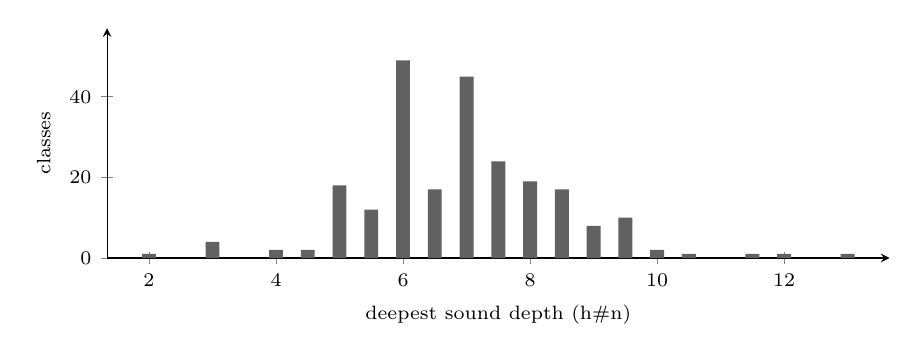
\begin{tikzpicture}
\begin{axis}[
  width=0.95\linewidth, height=45mm,
  ybar, bar width=5pt,
  xlabel={deepest sound depth (h\#n)}, ylabel={classes},
  ylabel near ticks, xlabel near ticks,
  ymin=0, ymax=57,
  tick label style={font=\scriptsize},
  label style={font=\scriptsize},
  axis lines=left, enlarge x limits=0.06,
]
\addplot[fill=black!62,draw=none] coordinates {(2.0,1) (3.0,4) (4.0,2) (4.5,2) (5.0,18) (5.5,12) (6.0,49) (6.5,17) (7.0,45) (7.5,24) (8.0,19) (8.5,17) (9.0,8) (9.5,10) (10.0,2) (10.5,1) (11.5,1) (12.0,1) (13.0,1)};
\end{axis}
\end{tikzpicture}
\end{center}

\section{The gap to the class maximum}

How much depth uniqueness costs: the class's longest helpmate minus
its deepest sound one, in plies. It is never zero.
\begin{center}
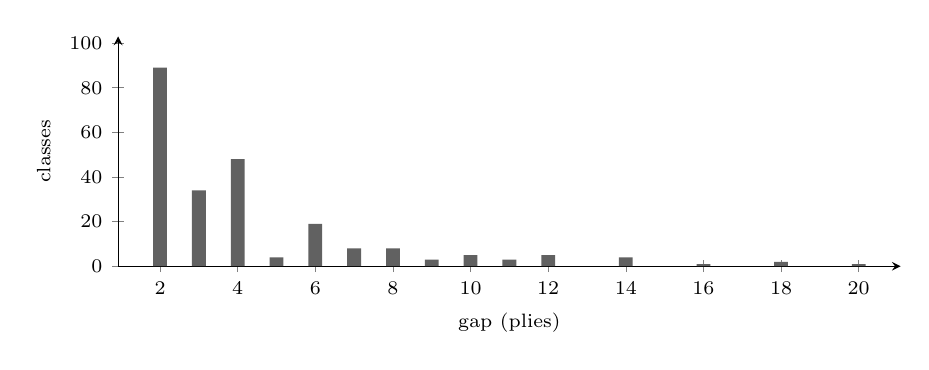
\begin{tikzpicture}
\begin{axis}[
  width=0.95\linewidth, height=45mm,
  ybar, bar width=5pt,
  xlabel={gap (plies)}, ylabel={classes},
  ylabel near ticks, xlabel near ticks,
  ymin=0, ymax=103,
  tick label style={font=\scriptsize},
  label style={font=\scriptsize},
  axis lines=left, enlarge x limits=0.06,
]
\addplot[fill=black!62,draw=none] coordinates {(2,89) (3,34) (4,48) (5,4) (6,19) (7,8) (8,8) (9,3) (10,5) (11,3) (12,5) (14,4) (16,1) (18,2) (20,1)};
\end{axis}
\end{tikzpicture}
\end{center}

Mean 4.4 plies, median 3,
worst 20 --- KRBvkp, which runs to
h\#16 but whose deepest sound
problem is only h\#6
(page~\pageref{hm:KRBvkp}).

\section{The ten deepest}

\begin{center}
\begin{tabular}{lrrrr}
\toprule
material & sound & class max & gap & positions \\
\midrule
KBvkrp & h\#13 & h\#16.5 & 7 & 2 \\
KBvkqp & h\#12 & h\#17 & 10 & 3 \\
KBvkbp & h\#11.5 & h\#16 & 9 & 8 \\
KBPvkp & h\#10.5 & h\#16 & 11 & 1 \\
KBvkqnn & h\#10 & h\#13 & 6 & 5 \\
KPvkpp & h\#10 & h\#15.5 & 11 & 2 \\
KBvknp & h\#9.5 & h\#15.5 & 12 & 2 \\
KBvkqbn & h\#9.5 & h\#12.5 & 6 & 90 \\
KBvkqn & h\#9.5 & h\#13 & 7 & 46 \\
KBvkqqn & h\#9.5 & h\#12.5 & 6 & 341 \\
\bottomrule
\end{tabular}
\end{center}

\section{Rarity}

At its deepest sound depth a class may hold a single position and
nothing else. 21 classes are like that, and
117 hold ten or fewer. Those are the positions with no
margin at all: change one man and the problem is gone.

\begin{center}
\begin{tabular}{llll}
\toprule
\multicolumn{4}{c}{classes with exactly one position at their deepest sound depth} \\
\midrule
KBPvkp~h\#10.5 & KNvkqb~h\#9.5 & KBBvkp~h\#9 & KNvknp~h\#8.5 \\
KNvkrn~h\#8.5 & KPvkqn~h\#8.5 & KBNvkq~h\#7.5 & KPPvkb~h\#7.5 \\
KPPvkn~h\#7.5 & KPPvkq~h\#7.5 & KPvkr~h\#7.5 & KBBNvk~h\#7 \\
KNNvkq~h\#7 & KNNvkr~h\#7 & KQBBvk~h\#7 & KRBBvk~h\#7 \\
KBBvk~h\#6.5 & KRvkqb~h\#6.5 & KQvkbn~h\#6 & KRRvkr~h\#6 \\
KRvk~h\#4.5 &  &  &  \\
\bottomrule
\end{tabular}
\end{center}

\chapter{Three men}
\markboth{Three men}{}

3 of the 5 material classes
with 3 men that can hold a mate, deepest sound problem first.

\hmentry{No.~1\quad KPvk}{KPvk}{6k1/8/8/8/8/8/4P3/2K5 w - - 0 1}{h\#6.5}{\textbf{h\#6.5}, unique solution.\\[0.3em]The class runs to h\#8.5, so the deepest sound problem is 4~plies shallower. Every position at that depth has a saturated solution count (255 or more).\\[0.3em]13 positions of the 86\,688 indexed have a unique solution at h\#6.5.\\[0.3em]\textit{Published:} Niemann, John -- Schachmatt, No. 427, 13/07/1947; Catalogue h\# (CHM) avec 6 pieces, No. 61, 1995; Wenigsteiner im Hilfsmatt, No. 77, 1977; Problemista, No. 1569, 07-10/1981, as h\#6 (P0530828); Ban, Jenö -- Magyar Sakkelet, 1961; Ideal-Mate Encyclopedia Vol.1, No. 12, 1999, as h\#7 0.1... (P1100755)}{1...e3 2.Kf7 e4 3.Ke6 e5 4.Kd5 e6 5.Kc4 e7 6.Kb3 e8=Q 7.Ka2 Qa4\#}{https://helpman.komtera.lt/?fen=6k1/8/8/8/8/8/4P3/2K5&moves=6.5}{2 + 1}{set-play, pure, model, ideal, mirror, promotion, excelsior, excelsior:white, single-piece, single-piece:white, single-piece:black, nocapture, nocheck, umnov, promotions:q}
\hmentry{No.~1b\quad KPvk}{KPvk-b}{8/8/8/1K6/8/3P4/7k/8 w - - 0 1}{h\#6.5}{\textbf{h\#6.5}, unique solution.\\[0.3em]Same material and stipulation as No.~1, which is published; this position is not in the published database, under any mirroring.}{1...d4 2.Kg3 d5 3.Kf4 d6 4.Ke5 d7 5.Kd6 Ka5 6.Kc7 Ka6 7.Kb8 d8=Q\#}{https://helpman.komtera.lt/?fen=8/8/8/1K6/8/3P4/7k/8&moves=6.5}{2 + 1}{pure, model, ideal, mirror, promotion, single-piece, single-piece:black, nocapture, nocheck, umnov, promotions:q}
\hmentry{No.~2\quad KQvk}{KQvk}{8/8/7k/6Q1/8/8/8/K7 b - - 0 1}{h\#6}{\textbf{h\#6}, unique solution.\\[0.3em]The class runs to h\#7, so the deepest sound problem is 2~plies shallower. Every position at that depth has a saturated solution count (255 or more).\\[0.3em]3 positions of the 29\,568 indexed have a unique solution at h\#6.\\[0.3em]\textit{Published:} Csaszar, Imre -- Magyar Sakkvilag, 1945; Ideal-Mate Review, 1990; Catalogue h\# (CHM) avec 6 pieces, No. 165, 1995, as h\#6 (P0551296)\\[0.3em]\textit{Note:} the side to move is in check in the diagram.}{1.Kh7 Kb2 2.Kh8 Kc3 3.Kh7 Kd4 4.Kh8 Ke5 5.Kh7 Kf6 6.Kh8 Qg7\#}{https://helpman.komtera.lt/?fen=8/8/7k/6Q1/8/8/8/K7&moves=6}{2 + 1}{pure, model, ideal, switchback, single-piece, single-piece:black, nocapture, nocheck}
\hmentry{No.~2b\quad KQvk}{KQvk-b}{8/7k/8/6Q1/8/8/8/K7 b - - 0 1}{h\#6}{\textbf{h\#6}, unique solution.\\[0.3em]Same material and stipulation as No.~2, which is published; this position is not in the published database, under any mirroring.}{1.Kh8 Kb2 2.Kh7 Kc3 3.Kh8 Kd4 4.Kh7 Ke5 5.Kh8 Kf6 6.Kh7 Qg7\#}{https://helpman.komtera.lt/?fen=8/7k/8/6Q1/8/8/8/K7&moves=6}{2 + 1}{set-play, switchback, single-piece, single-piece:black, pendulum, nocapture, nocheck}
\hmentry{No.~3\quad KRvk}{KRvk}{4k3/8/8/8/8/8/2R5/1K6 w - - 0 1}{h\#4.5}{\textbf{h\#4.5}, unique solution.\\[0.3em]The class runs to h\#7, so the deepest sound problem is 5~plies shallower. Every position at that depth has a saturated solution count (255 or more).\\[0.3em]1 position of the 29\,568 indexed has a unique solution at h\#4.5.\\[0.3em]\textit{Published:} Ban, Jenö -- Diagramme und Figuren, No. 1295, 27/11/1965; Catalogue h\# (CHM) avec 6 pieces, No. 122, 1995; Ideal-Mate Encyclopedia Vol.1, No. 1848, 1999, as h\#5 0.1... (P0531991)}{1...Kc1 2.Kf7 Kd2 3.Kg6 Ke3 4.Kh5 Kf4 5.Kh4 Rh2\#}{https://helpman.komtera.lt/?fen=4k3/8/8/8/8/8/2R5/1K6&moves=4.5}{2 + 1}{pure, model, ideal, mirror, single-piece, single-piece:black, nocapture, nocheck}

\chapter{Four men}
\markboth{Four men}{}

37 of the 40 material classes
with 4 men that can hold a mate, deepest sound problem first.

\hmentry{No.~4\quad KPvkp}{KPvkp}{8/8/p7/8/P7/8/3K4/7k w - - 0 1}{h\#8.5}{\textbf{h\#8.5}, unique solution.\\[0.3em]The class runs to h\#14.5, so the deepest sound problem is 12~plies shallower. Every position at that depth has a saturated solution count (255 or more).\\[0.3em]2 positions of the 4\,161\,024 indexed have a unique solution at h\#8.5.}{1...Kc3 2.Kg2 Kb4 3.a5+ Kxa5 4.Kf3 Kb4 5.Ke4 a5 6.Kd5 a6 7.Kc6 a7 8.Kb7 Kc5 9.Ka6 a8=Q\#}{https://helpman.komtera.lt/?fen=8/8/p7/8/P7/8/3K4/7k&moves=8.5}{2 + 2}{pure, model, ideal, mirror, promotion, switchback, promotions:q}
\hmentry{No.~5\quad KBvkn}{KBvkn}{8/8/8/8/8/1k6/5n2/1K5B b - - 0 1}{h\#8}{\textbf{h\#8}, unique solution.\\[0.3em]The class runs to h\#12, so the deepest sound problem is 8~plies shallower. Every position at that depth has a saturated solution count (255 or more).\\[0.3em]19 positions of the 1\,892\,352 indexed have a unique solution at h\#8.}{1.Kc3 Bg2 2.Kd2 Bf1 3.Ke1 Kc2 4.Nh3 Kd3 5.Kf2 Ke4 6.Kg1 Kf3 7.Kh1 Kg3 8.Ng1 Bg2\#}{https://helpman.komtera.lt/?fen=8/8/8/8/8/1k6/5n2/1K5B&moves=8}{2 + 2}{pure, model, ideal, switchback, self-block, nocapture, nocheck}
\hmentry{No.~6\quad KBvkp}{KBvkp}{8/8/8/4k3/2p5/8/8/K3B3 b - - 0 1}{h\#8}{\textbf{h\#8}, unique solution.\\[0.3em]The class runs to h\#16, so the deepest sound problem is 16~plies shallower. Every position at that depth has a saturated solution count (255 or more).\\[0.3em]16 positions of the 5\,548\,032 indexed have a unique solution at h\#8.}{1.c3 Bh4 2.c2 Kb2 3.c1=N Kc2 4.Kd4 Kd1 5.Kc3 Be7 6.Kb2 Ba3+ 7.Ka1 Kc2 8.Na2 Bb2\#}{https://helpman.komtera.lt/?fen=8/8/8/4k3/2p5/8/8/K3B3&moves=8}{2 + 2}{pure, model, ideal, promotion, underpromotion, switchback, self-block, nocapture, umnov, promotions:n}
\hmentry{No.~7\quad KNvkb}{KNvkb}{8/8/7k/8/8/1b6/4N3/K7 b - - 0 1}{h\#8}{\textbf{h\#8}, unique solution.\\[0.3em]The class runs to h\#10.5, so the deepest sound problem is 5~plies shallower. Every position at that depth has a saturated solution count (255 or more).\\[0.3em]5 positions of the 1\,892\,352 indexed have a unique solution at h\#8.}{1.Kg5 Nd4 2.Kf4 Kb2 3.Ke3 Ka3 4.Kd2 Kb4 5.Kc1 Kc3 6.Kb1 Kd2 7.Ka1 Kc1 8.Ba2 Nc2\#}{https://helpman.komtera.lt/?fen=8/8/7k/8/8/1b6/4N3/K7&moves=8}{2 + 2}{pure, model, ideal, self-block, nocapture, nocheck}
\hmentry{No.~8\quad KNvkp}{KNvkp}{8/8/3p4/8/8/1k6/N7/K7 b - - 0 1}{h\#8}{\textbf{h\#8}, unique solution.\\[0.3em]The class runs to h\#11.5, so the deepest sound problem is 7~plies shallower. Every position at that depth has a saturated solution count (255 or more).\\[0.3em]4 positions of the 5\,548\,032 indexed have a unique solution at h\#8.}{1.d5 Kb1 2.d4 Kc1 3.d3 Kd2 4.Kb2 Nb4 5.Ka1 Kc3 6.d2 Kb3 7.d1=R Ka3 8.Rb1 Nc2\#}{https://helpman.komtera.lt/?fen=8/8/3p4/8/8/1k6/N7/K7&moves=8}{2 + 2}{pure, model, ideal, promotion, underpromotion, self-block, nocapture, nocheck, umnov, promotions:r}
\hmentry{No.~9\quad KNvkr}{KNvkr}{8/8/8/8/8/7k/5r1N/K7 b - - 0 1}{h\#8}{\textbf{h\#8}, unique solution.\\[0.3em]The class runs to h\#9.5, so the deepest sound problem is 3~plies shallower. Every position at that depth has a saturated solution count (255 or more).\\[0.3em]9 positions of the 1\,892\,352 indexed have a unique solution at h\#8.\\[0.3em]\textit{Published:} Elkies, Noam D. -- Variantim, No. 546, 11/1995, as h\#8 (P0543062); Mertes, Helmut -- feenschach, 01/1977; Ideal-Mate Encyclopedia Vol.1, No. 400, 1999, as h\#8 (P0543063)}{1.Kg2 Nf3 2.Kf1 Kb1 3.Ke2 Kb2 4.Kd3+ Kc1 5.Kc3 Kd1 6.Kb2 Nd4 7.Ka1 Kc1 8.Ra2 Nb3\#}{https://helpman.komtera.lt/?fen=8/8/8/8/8/7k/5r1N/K7&moves=8}{2 + 2}{pure, model, ideal, switchback, self-block, nocapture}
\hmentry{No.~9b\quad KNvkr}{KNvkr-b}{8/7k/N7/8/8/8/4r3/1K6 b - - 0 1}{h\#8}{\textbf{h\#8}, unique solution.\\[0.3em]Same material and stipulation as No.~9, which is published; this position is not in the published database, under any mirroring.}{1.Kg6 Nb4 2.Kf5 Nc2 3.Ke4 Kb2 4.Kd3 Kc1 5.Kc3 Kd1 6.Kb2 Nd4 7.Ka1 Kc1 8.Ra2 Nb3\#}{https://helpman.komtera.lt/?fen=8/7k/N7/8/8/8/4r3/1K6&moves=8}{2 + 2}{pure, model, ideal, switchback, self-block, nocapture, nocheck}
\hmentry{No.~10\quad KNvkn}{KNvkn}{5n2/8/8/8/8/8/3k2N1/K7 w - - 0 1}{h\#7.5}{\textbf{h\#7.5}, unique solution.\\[0.3em]The class runs to h\#10, so the deepest sound problem is 5~plies shallower. Every position at that depth has a saturated solution count (255 or more).\\[0.3em]14 positions of the 1\,892\,352 indexed have a unique solution at h\#7.5.\\[0.3em]\textit{Published:} Kotesovec, Vaclav -- Sachova skladba, No. 1065, 06/1987, as h\#8 0.1... (P0542897); ?, ? -- ?, 03/1975, as h\#8 0.1... (P0542908)}{1...Nh4 2.Ke3 Kb2 3.Kf4 Kc3 4.Kg5 Kd4 5.Kh6 Ke5 6.Kh7 Kf6 7.Kh8 Kf7 8.Nh7 Ng6\#}{https://helpman.komtera.lt/?fen=5n2/8/8/8/8/8/3k2N1/K7&moves=7.5}{2 + 2}{pure, model, ideal, self-block, nocapture, nocheck}
\hmentry{No.~10b\quad KNvkn}{KNvkn-b}{5n2/8/8/8/6N1/8/3k4/1K6 w - - 0 1}{h\#7.5}{\textbf{h\#7.5}, unique solution.\\[0.3em]Same material and stipulation as No.~10, which is published; this position is not in the published database, under any mirroring.}{1...Ne5 2.Ke3 Kc2 3.Kf4 Kd3 4.Kg5 Ke4 5.Kh6 Kf5 6.Kh7 Kf6 7.Kh8 Kf7 8.Nh7 Ng6\#}{https://helpman.komtera.lt/?fen=5n2/8/8/8/6N1/8/3k4/1K6&moves=7.5}{2 + 2}{pure, model, ideal, self-block, nocapture, nocheck}
\hmentry{No.~11\quad KPvkb}{KPvkb}{8/8/1K6/8/2b5/2P5/7k/8 w - - 0 1}{h\#7.5}{\textbf{h\#7.5}, unique solution.\\[0.3em]The class runs to h\#8.5, so the deepest sound problem is 2~plies shallower. Every position at that depth has a saturated solution count (255 or more).\\[0.3em]13 positions of the 5\,548\,032 indexed have a unique solution at h\#7.5.}{1...Ka5 2.Bd5 c4 3.Kg3 cxd5 4.Kf4 d6 5.Ke5 d7 6.Kd6 Kb5 7.Kc7 Ka6 8.Kb8 d8=Q\#}{https://helpman.komtera.lt/?fen=8/8/1K6/8/2b5/2P5/7k/8&moves=7.5}{2 + 2}{set-play, pure, model, ideal, mirror, promotion, nocheck, umnov, promotions:q}
\hmentry{No.~12\quad KPvkn}{KPvkn}{K7/8/8/n7/2P5/8/8/7k w - - 0 1}{h\#7.5}{\textbf{h\#7.5}, unique solution.\\[0.3em]The class runs to h\#8.5, so the deepest sound problem is 2~plies shallower. Every position at that depth has a saturated solution count (255 or more).\\[0.3em]8 positions of the 5\,548\,032 indexed have a unique solution at h\#7.5.}{1...c5 2.Kg2 c6 3.Kf3 c7 4.Ke4 c8=Q 5.Kd5 Qf5+ 6.Kc6 Kb8 7.Kb6 Kc8 8.Ka7 Qxa5\#}{https://helpman.komtera.lt/?fen=K7/8/8/n7/2P5/8/8/7k&moves=7.5}{2 + 2}{pure, model, ideal, mirror, promotion, single-piece, single-piece:black, promotions:q}
\hmentry{No.~13\quad KPvkq}{KPvkq}{8/K7/8/8/8/8/3P4/2q4k w - - 0 1}{h\#7.5}{\textbf{h\#7.5}, unique solution.\\[0.3em]The class runs to h\#9, so the deepest sound problem is 3~plies shallower. Every position at that depth has a saturated solution count (255 or more).\\[0.3em]32 positions of the 5\,548\,032 indexed have a unique solution at h\#7.5.}{1...d4 2.Kg2 d5 3.Kf3 d6 4.Ke4 d7 5.Kd5 d8=Q+ 6.Kc6 Qd5+ 7.Kc7 Ka6 8.Kb8 Qb7\#}{https://helpman.komtera.lt/?fen=8/K7/8/8/8/8/3P4/2q4k&moves=7.5}{2 + 2}{promotion, excelsior, excelsior:white, closed-walk, single-piece, single-piece:black, nocapture, umnov, promotions:q}
\hmentry{No.~14\quad KPvkr}{KPvkr}{8/7k/8/8/8/7r/1K5P/8 w - - 0 1}{h\#7.5}{\textbf{h\#7.5}, unique solution.\\[0.3em]The class runs to h\#8.5, so the deepest sound problem is 2~plies shallower. Every position at that depth has a saturated solution count (255 or more).\\[0.3em]1 position of the 5\,548\,032 indexed has a unique solution at h\#7.5.\\[0.3em]\textit{Published:} Maslar, Zdravko -- ?,, as h\#8 0.1... (P0542623)}{1...Ka2 2.Ra3+ Kxa3 3.Kg6 h4 4.Kf5 h5 5.Ke4 h6 6.Kd3 h7 7.Kc2 h8=Q 8.Kb1 Qb2\#}{https://helpman.komtera.lt/?fen=8/7k/8/8/8/7r/1K5P/8&moves=7.5}{2 + 2}{set-play, promotion, excelsior, excelsior:white, promotions:q}
\hmentry{No.~15\quad KBPvk}{KBPvk}{7k/8/8/8/B7/8/P7/3K4 b - - 0 1}{h\#7}{\textbf{h\#7}, unique solution.\\[0.3em]The class runs to h\#8, so the deepest sound problem is 2~plies shallower. Every position at that depth has a saturated solution count (255 or more).\\[0.3em]12 positions of the 5\,548\,032 indexed have a unique solution at h\#7.\\[0.3em]\textit{Published:} Elkies, Noam D. -- The Problemist, No. H2794, 07/2004, as h\#7 (P1187767)}{1.Kg7 Bb3 2.Kf6 a4 3.Ke5 a5 4.Kd4 a6 5.Kc3 a7 6.Kb2 a8=Q 7.Kb1 Qa2\#}{https://helpman.komtera.lt/?fen=7k/8/8/8/B7/8/P7/3K4&moves=7}{3 + 1}{promotion, excelsior, excelsior:white, closed-walk, single-piece, single-piece:black, nocapture, nocheck, promotions:q}
\hmentry{No.~15b\quad KBPvk}{KBPvk-b}{7k/8/8/8/B7/P7/8/3K4 b - - 0 1}{h\#7}{\textbf{h\#7}, unique solution.\\[0.3em]Same material and stipulation as No.~15, which is published; this position is not in the published database, under any mirroring.}{1.Kg7 Bb3 2.Kf6 a4 3.Ke5 a5 4.Kd4 a6 5.Kc3 a7 6.Kb2 a8=Q 7.Kb1 Qa2\#}{https://helpman.komtera.lt/?fen=7k/8/8/8/B7/P7/8/3K4&moves=7}{3 + 1}{promotion, single-piece, single-piece:black, nocapture, nocheck, promotions:q}
\hmentry{No.~16\quad KNPvk}{KNPvk}{8/8/8/8/8/N7/P7/3K3k b - - 0 1}{h\#7}{\textbf{h\#7}, unique solution.\\[0.3em]The class runs to h\#8.5, so the deepest sound problem is 3~plies shallower. Every position at that depth has a saturated solution count (255 or more).\\[0.3em]49 positions of the 5\,548\,032 indexed have a unique solution at h\#7.\\[0.3em]\textit{Published:} Elkies, Noam D. -- The Problemist, No. H2793, 07/2004, as h\#7 (P1187769)}{1.Kg2 Nc2 2.Kf3 a4 3.Ke4 a5 4.Kd3 a6 5.Kc3 a7 6.Kb2 a8=Q 7.Kb1 Qa1\#}{https://helpman.komtera.lt/?fen=8/8/8/8/8/N7/P7/3K3k&moves=7}{3 + 1}{promotion, excelsior, excelsior:white, single-piece, single-piece:black, nocapture, nocheck, promotions:q}
\hmentry{No.~16b\quad KNPvk}{KNPvk-b}{8/8/8/8/8/KN6/P7/7k b - - 0 1}{h\#7}{\textbf{h\#7}, unique solution.\\[0.3em]Same material and stipulation as No.~16, which is published; this position is not in the published database, under any mirroring.}{1.Kg2 Kb4 2.Kf3 a4 3.Ke4 a5 4.Kd5 a6 5.Kc6 a7 6.Kb7 Kc5 7.Ka6 a8=Q\#}{https://helpman.komtera.lt/?fen=8/8/8/8/8/KN6/P7/7k&moves=7}{3 + 1}{mirror, promotion, excelsior, excelsior:white, single-piece, single-piece:black, nocapture, nocheck, promotions:q}
\hmentry{No.~17\quad KPPvk}{KPPvk}{8/7k/8/8/8/6P1/K5P1/8 b - - 0 1}{h\#7}{\textbf{h\#7}, unique solution.\\[0.3em]The class runs to h\#8, so the deepest sound problem is 2~plies shallower. Every position at that depth has a saturated solution count (255 or more).\\[0.3em]2 positions of the 4\,161\,024 indexed have a unique solution at h\#7.\\[0.3em]\textit{Published:} Salazar Lopez, Francisco -- British Chess Magazine, 03/1973; Catalogue h\# (CHM) avec 6 pieces, No. 213, 1995; The Problemist, 05/2005; Problemkiste, No. G), 01/2010, as h\#7 (P0545149)}{1.Kg6 Ka3 2.Kf5 g4+ 3.Ke4 g5 4.Kd3 g6 5.Kc2 g7 6.Kb1 g8=Q 7.Ka1 Qa2\#}{https://helpman.komtera.lt/?fen=8/7k/8/8/8/6P1/K5P1/8&moves=7}{3 + 1}{promotion, single-piece, single-piece:black, nocapture, promotions:q}
\hmentry{No.~18\quad KQPvk}{KQPvk}{6Qk/8/8/8/8/8/4P3/2K5 b - - 0 1}{h\#7}{\textbf{h\#7}, unique solution.\\[0.3em]The class runs to h\#8, so the deepest sound problem is 2~plies shallower.\\[0.3em]12 positions of the 5\,548\,032 indexed have a unique solution at h\#7.\\[0.3em]\textit{Note:} the side to move is in check in the diagram; the solution begins with a capture.}{1.Kxg8 e3 2.Kf7 e4 3.Ke6 e5 4.Kd5 e6 5.Kc4 e7 6.Kb3 e8=Q 7.Ka2 Qa4\#}{https://helpman.komtera.lt/?fen=6Qk/8/8/8/8/8/4P3/2K5&moves=7}{3 + 1}{pure, model, ideal, mirror, promotion, excelsior, excelsior:white, single-piece, single-piece:white, single-piece:black, phoenix, nocheck, umnov, promotions:q}
\hmentry{No.~19\quad KBBvk}{KBBvk}{7k/8/7B/8/8/8/2B5/K7 w - - 0 1}{h\#6.5}{\textbf{h\#6.5}, unique solution.\\[0.3em]The class runs to h\#8, so the deepest sound problem is 3~plies shallower. Every position at that depth has a saturated solution count (255 or more).\\[0.3em]1 position of the 1\,892\,352 indexed has a unique solution at h\#6.5.\\[0.3em]\textit{Published:} Maslar, Zdravko -- feenschach, 01-03/1978; Catalogue h\# (CHM) avec 6 pieces, No. 899, 1995; Problemkiste, No. A1, 03/2012, as h\#7 0.1... (P0545758)}{1...Kb2 2.Kg8 Kc3 3.Kf7 Kd3 4.Kg6 Ke4 5.Kh5 Kf5 6.Kh4 Bg5+ 7.Kh5 Bd1\#}{https://helpman.komtera.lt/?fen=7k/8/7B/8/8/8/2B5/K7&moves=6.5}{3 + 1}{switchback, single-piece, single-piece:black, nocapture}
\hmentry{No.~20\quad KBvkb}{KBvkb}{8/8/6b1/8/8/6k1/3B4/K7 w - - 0 1}{h\#6.5}{\textbf{h\#6.5}, unique solution.\\[0.3em]The class runs to h\#10, so the deepest sound problem is 7~plies shallower. Every position at that depth has a saturated solution count (255 or more).\\[0.3em]8 positions of the 1\,892\,352 indexed have a unique solution at h\#6.5.}{1...Kb2 2.Kg4 Kc3 3.Kf5 Kd4 4.Kf6 Bc3 5.Kg7 Ke5 6.Kh8 Kf6 7.Bh7 Kf7\#}{https://helpman.komtera.lt/?fen=8/8/6b1/8/8/6k1/3B4/K7&moves=6.5}{2 + 2}{self-block, nocapture, nocheck}
\hmentry{No.~21\quad KNNvk}{KNNvk}{1k5N/8/8/8/8/8/7N/3K4 w - - 0 1}{h\#6.5}{\textbf{h\#6.5}, unique solution.\\[0.3em]The class runs to h\#8, so the deepest sound problem is 3~plies shallower. Every position at that depth has a saturated solution count (255 or more).\\[0.3em]9 positions of the 1\,892\,352 indexed have a unique solution at h\#6.5.\\[0.3em]\textit{Published:} Bebesi, Gyula -- Diagramme und Figuren, No. 1910, 12/12/1966; Catalogue h\# (CHM) avec 6 pieces, No. 624, 1995; Ideal-Mate Encyclopedia Vol.1, No. 930, 1999, as h\#7 0.1... (P0545484)}{1...Ke2 2.Kc7 Kf3 3.Kd6 Kg4 4.Ke5 Kh5 5.Kf4 Ng6+ 6.Kg3 Nf1+ 7.Kh3 Nf4\#}{https://helpman.komtera.lt/?fen=1k5N/8/8/8/8/8/7N/3K4&moves=6.5}{3 + 1}{pure, model, ideal, mirror, single-piece, single-piece:black, nocapture}
\hmentry{No.~21b\quad KNNvk}{KNNvk-b}{6kN/8/8/8/8/8/7N/3K4 w - - 0 1}{h\#6.5}{\textbf{h\#6.5}, unique solution.\\[0.3em]Same material and stipulation as No.~21, which is published; this position is not in the published database, under any mirroring.}{1...Ke2 2.Kg7 Kf3 3.Kf6 Kg4 4.Ke5 Kh5 5.Kf4 Ng6+ 6.Kg3 Nf1+ 7.Kh3 Nf4\#}{https://helpman.komtera.lt/?fen=6kN/8/8/8/8/8/7N/3K4&moves=6.5}{3 + 1}{pure, model, ideal, mirror, single-piece, single-piece:black, nocapture}
\hmentry{No.~22\quad KBNvk}{KBNvk}{8/6N1/8/8/8/2B5/8/K2k4 b - - 0 1}{h\#6}{\textbf{h\#6}, unique solution.\\[0.3em]The class runs to h\#8, so the deepest sound problem is 4~plies shallower. Every position at that depth has a saturated solution count (255 or more).\\[0.3em]23 positions of the 1\,892\,352 indexed have a unique solution at h\#6.}{1.Kc2 Ka2 2.Kc1 Kb3 3.Kb1 Kc4 4.Ka2 Ne6 5.Ka3 Bb4+ 6.Ka4 Nc5\#}{https://helpman.komtera.lt/?fen=8/6N1/8/8/8/2B5/8/K2k4&moves=6}{3 + 1}{set-play, single-piece, single-piece:black, nocapture}
\hmentry{No.~23\quad KQBvk}{KQBvk}{7B/7k/8/6Q1/8/8/8/K7 b - - 0 1}{h\#6}{\textbf{h\#6}, unique solution.\\[0.3em]The class runs to h\#7, so the deepest sound problem is 2~plies shallower. Every position at that depth has a saturated solution count (255 or more).\\[0.3em]3 positions of the 1\,892\,352 indexed have a unique solution at h\#6.\\[0.3em]\textit{Note:} the solution begins with a capture.}{1.Kxh8 Kb2 2.Kh7 Kc3 3.Kh8 Kd4 4.Kh7 Ke5 5.Kh8 Kf6 6.Kh7 Qg7\#}{https://helpman.komtera.lt/?fen=7B/7k/8/6Q1/8/8/8/K7&moves=6}{3 + 1}{switchback, single-piece, single-piece:black, pendulum, nocheck}
\hmentry{No.~24\quad KQNvk}{KQNvk}{7N/7k/8/6Q1/8/8/8/K7 b - - 0 1}{h\#6}{\textbf{h\#6}, unique solution.\\[0.3em]The class runs to h\#7, so the deepest sound problem is 2~plies shallower. Every position at that depth has a saturated solution count (255 or more).\\[0.3em]3 positions of the 1\,892\,352 indexed have a unique solution at h\#6.\\[0.3em]\textit{Note:} the solution begins with a capture.}{1.Kxh8 Kb2 2.Kh7 Kc3 3.Kh8 Kd4 4.Kh7 Ke5 5.Kh8 Kf6 6.Kh7 Qg7\#}{https://helpman.komtera.lt/?fen=7N/7k/8/6Q1/8/8/8/K7&moves=6}{3 + 1}{switchback, single-piece, single-piece:black, pendulum, nocheck}
\hmentry{No.~25\quad KQQvk}{KQQvk}{7Q/7k/8/6Q1/8/8/8/K7 b - - 0 1}{h\#6}{\textbf{h\#6}, unique solution.\\[0.3em]The class runs to h\#7, so the deepest sound problem is 2~plies shallower. Every position at that depth has a saturated solution count (255 or more).\\[0.3em]2 positions of the 1\,892\,352 indexed have a unique solution at h\#6.\\[0.3em]\textit{Note:} the side to move is in check in the diagram; the solution begins with a capture.}{1.Kxh8 Kb2 2.Kh7 Kc3 3.Kh8 Kd4 4.Kh7 Ke5 5.Kh8 Kf6 6.Kh7 Qg7\#}{https://helpman.komtera.lt/?fen=7Q/7k/8/6Q1/8/8/8/K7&moves=6}{3 + 1}{switchback, single-piece, single-piece:black, pendulum, nocheck}
\hmentry{No.~26\quad KQRvk}{KQRvk}{7R/7k/8/6Q1/8/8/8/K7 b - - 0 1}{h\#6}{\textbf{h\#6}, unique solution.\\[0.3em]The class runs to h\#7, so the deepest sound problem is 2~plies shallower. Every position at that depth has a saturated solution count (255 or more).\\[0.3em]2 positions of the 1\,892\,352 indexed have a unique solution at h\#6.\\[0.3em]\textit{Note:} the side to move is in check in the diagram; the solution begins with a capture.}{1.Kxh8 Kb2 2.Kh7 Kc3 3.Kh8 Kd4 4.Kh7 Ke5 5.Kh8 Kf6 6.Kh7 Qg7\#}{https://helpman.komtera.lt/?fen=7R/7k/8/6Q1/8/8/8/K7&moves=6}{3 + 1}{switchback, single-piece, single-piece:black, pendulum, nocheck}
\hmentry{No.~27\quad KQvkn}{KQvkn}{7k/8/8/6Q1/8/8/1n6/K7 b - - 0 1}{h\#6}{\textbf{h\#6}, unique solution.\\[0.3em]The class runs to h\#7, so the deepest sound problem is 2~plies shallower. Every position at that depth has a saturated solution count (255 or more).\\[0.3em]4 positions of the 1\,892\,352 indexed have a unique solution at h\#6.}{1.Kh7 Kxb2 2.Kh8 Kc3 3.Kh7 Kd4 4.Kh8 Ke5 5.Kh7 Kf6 6.Kh8 Qg7\#}{https://helpman.komtera.lt/?fen=7k/8/8/6Q1/8/8/1n6/K7&moves=6}{2 + 2}{set-play, pure, model, ideal, switchback, single-piece, single-piece:black, pendulum, nocheck}
\hmentry{No.~28\quad KQvkp}{KQvkp}{K7/1p6/8/8/8/8/4Q3/5k2 b - - 0 1}{h\#6}{\textbf{h\#6}, unique solution.\\[0.3em]The class runs to h\#7, so the deepest sound problem is 2~plies shallower. Every position at that depth has a saturated solution count (255 or more).\\[0.3em]4 positions of the 5\,548\,032 indexed have a unique solution at h\#6.\\[0.3em]\textit{Note:} the side to move is in check in the diagram.}{1.Kg1 Kxb7 2.Kh1 Kc6 3.Kg1 Kd5 4.Kh1 Ke4 5.Kg1 Kf3 6.Kh1 Qg2\#}{https://helpman.komtera.lt/?fen=K7/1p6/8/8/8/8/4Q3/5k2&moves=6}{2 + 2}{pure, model, ideal, switchback, single-piece, single-piece:black, nocheck}
\hmentry{No.~29\quad KRBvk}{KRBvk}{6R1/8/7k/8/8/8/8/K2B4 b - - 0 1}{h\#6}{\textbf{h\#6}, unique solution.\\[0.3em]The class runs to h\#7, so the deepest sound problem is 2~plies shallower.\\[0.3em]20 positions of the 1\,892\,352 indexed have a unique solution at h\#6.}{1.Kh7 Kb2 2.Kh6 Kc3 3.Kh7 Kd4 4.Kh6 Ke5 5.Kh7 Kf6 6.Kh6 Rh8\#}{https://helpman.komtera.lt/?fen=6R1/8/7k/8/8/8/8/K2B4&moves=6}{3 + 1}{set-play, mirror, switchback, single-piece, single-piece:black, pendulum, nocapture, nocheck}
\hmentry{No.~30\quad KRPvk}{KRPvk}{8/7k/6R1/8/8/8/P7/K7 b - - 0 1}{h\#6}{\textbf{h\#6}, unique solution.\\[0.3em]The class runs to h\#8, so the deepest sound problem is 4~plies shallower. Every position at that depth has a saturated solution count (255 or more).\\[0.3em]25 positions of the 5\,548\,032 indexed have a unique solution at h\#6.}{1.Kh8 a4 2.Kh7 a5 3.Kh8 a6 4.Kh7 a7 5.Kh8 a8=Q+ 6.Kh7 Qg8\#}{https://helpman.komtera.lt/?fen=8/7k/6R1/8/8/8/P7/K7&moves=6}{3 + 1}{promotion, excelsior, excelsior:white, switchback, single-piece, single-piece:white, single-piece:black, pendulum, nocapture, promotions:q}
\hmentry{No.~31\quad KRvkp}{KRvkp}{8/8/7k/6R1/8/1p6/8/K7 b - - 0 1}{h\#6}{\textbf{h\#6}, unique solution.\\[0.3em]The class runs to h\#7, so the deepest sound problem is 2~plies shallower. Every position at that depth has a saturated solution count (255 or more).\\[0.3em]84 positions of the 5\,548\,032 indexed have a unique solution at h\#6.}{1.Kh7 Kb2 2.Kh8 Kc3 3.b2 Kd4 4.b1=R Ke5 5.Rb8 Kf6 6.Rg8 Rh5\#}{https://helpman.komtera.lt/?fen=8/8/7k/6R1/8/1p6/8/K7&moves=6}{2 + 2}{set-play, pure, model, ideal, promotion, underpromotion, self-block, nocapture, nocheck, umnov, promotions:r}
\hmentry{No.~32\quad KQvkq}{KQvkq}{8/8/5k2/8/6Q1/q7/8/K7 w - - 0 1}{h\#5.5}{\textbf{h\#5.5}, unique solution.\\[0.3em]The class runs to h\#7, so the deepest sound problem is 3~plies shallower. Every position at that depth has a saturated solution count (255 or more).\\[0.3em]7 positions of the 1\,892\,352 indexed have a unique solution at h\#5.5.\\[0.3em]\textit{Published:} Sheglow, Wiktor S. -- Suomen Tehtäväniekat, No. (257), 05-06/1998, as h\#6 0.1... (P0574108)\\[0.3em]\textit{Note:} the side to move is in check in the diagram.}{1...Kb1 2.Qd3+ Kc1 3.Qg6 Kd2 4.Kg7 Ke3 5.Kh6 Kf4 6.Qh7 Qg5\#}{https://helpman.komtera.lt/?fen=8/8/5k2/8/6Q1/q7/8/K7&moves=5.5}{2 + 2}{pure, model, ideal, self-block, nocapture}
\hmentry{No.~32b\quad KQvkq}{KQvkq-b}{8/7k/8/6Q1/8/8/1q6/K7 w - - 0 1}{h\#5.5}{\textbf{h\#5.5}, unique solution.\\[0.3em]Same material and stipulation as No.~32, which is published; this position is not in the published database, under any mirroring.\\[0.3em]\textit{Note:} the side to move is in check in the diagram; the solution begins with a capture.}{1...Kxb2 2.Kh8 Kc3 3.Kh7 Kd4 4.Kh8 Ke5 5.Kh7 Kf6 6.Kh8 Qg7\#}{https://helpman.komtera.lt/?fen=8/7k/8/6Q1/8/8/1q6/K7&moves=5.5}{2 + 2}{pure, model, ideal, switchback, single-piece, single-piece:black, pendulum, nocheck}
\hmentry{No.~33\quad KRvkq}{KRvkq}{8/8/5k2/8/8/6R1/5q2/K7 w - - 0 1}{h\#5.5}{\textbf{h\#5.5}, unique solution.\\[0.3em]The class runs to h\#7.5, so the deepest sound problem is 4~plies shallower. Every position at that depth has a saturated solution count (255 or more).\\[0.3em]6 positions of the 1\,892\,352 indexed have a unique solution at h\#5.5.}{1...Kb1 2.Qf5+ Kc1 3.Qg6 Kd2 4.Kg7 Ke3 5.Kh6 Kf4 6.Kh5 Rh3\#}{https://helpman.komtera.lt/?fen=8/8/5k2/8/8/6R1/5q2/K7&moves=5.5}{2 + 2}{pure, model, ideal, self-block, nocapture}
\hmentry{No.~34\quad KRvkr}{KRvkr}{8/8/5k2/8/6R1/8/7r/K7 w - - 0 1}{h\#5.5}{\textbf{h\#5.5}, unique solution.\\[0.3em]The class runs to h\#7, so the deepest sound problem is 3~plies shallower. Every position at that depth has a saturated solution count (255 or more).\\[0.3em]9 positions of the 1\,892\,352 indexed have a unique solution at h\#5.5.}{1...Kb1 2.Rh6 Kc2 3.Rg6 Kd3 4.Kg7 Ke4 5.Kh6 Kf5 6.Rg7 Rh4\#}{https://helpman.komtera.lt/?fen=8/8/5k2/8/6R1/8/7r/K7&moves=5.5}{2 + 2}{pure, model, ideal, self-block, nocapture, nocheck}
\hmentry{No.~35\quad KQvkb}{KQvkb}{8/8/7k/8/8/b5Q1/8/K7 b - - 0 1}{h\#5}{\textbf{h\#5}, unique solution.\\[0.3em]The class runs to h\#6, so the deepest sound problem is 2~plies shallower.\\[0.3em]64 positions of the 1\,892\,352 indexed have a unique solution at h\#5.}{1.Kh5 Qxa3 2.Kg4 Qa2 3.Kf3 Kb2 4.Ke2 Kc3+ 5.Kd1 Qd2\#}{https://helpman.komtera.lt/?fen=8/8/7k/8/8/b5Q1/8/K7&moves=5}{2 + 2}{single-piece, single-piece:black}
\hmentry{No.~36\quad KQvkr}{KQvkr}{8/8/8/8/7k/1r4Q1/8/K7 b - - 0 1}{h\#5}{\textbf{h\#5}, unique solution.\\[0.3em]The class runs to h\#6, so the deepest sound problem is 2~plies shallower. Every position at that depth has a saturated solution count (255 or more).\\[0.3em]7 positions of the 1\,892\,352 indexed have a unique solution at h\#5.\\[0.3em]\textit{Note:} the side to move is in check in the diagram.}{1.Kh5 Qxb3 2.Kg4 Qa2 3.Kf3 Kb2 4.Ke2 Kc3+ 5.Kd1 Qd2\#}{https://helpman.komtera.lt/?fen=8/8/8/8/7k/1r4Q1/8/K7&moves=5}{2 + 2}{single-piece, single-piece:black}
\hmentry{No.~37\quad KRNvk}{KRNvk}{8/8/8/8/6k1/N4R2/8/K7 b - - 0 1}{h\#5}{\textbf{h\#5}, unique solution.\\[0.3em]The class runs to h\#7, so the deepest sound problem is 4~plies shallower. Every position at that depth has a saturated solution count (255 or more).\\[0.3em]19 positions of the 1\,892\,352 indexed have a unique solution at h\#5.\\[0.3em]\textit{Published:} Maslar, Zdravko -- Stern, 15/01/1981; Catalogue h\# (CHM) avec 6 pieces, No. 784, 1995, as h\#5 (P0545644)}{1.Kg5 Rb3 2.Kf4 Rb2 3.Ke3 Nc2+ 4.Kd2 Ne3+ 5.Kc1 Rc2\#}{https://helpman.komtera.lt/?fen=8/8/8/8/6k1/N4R2/8/K7&moves=5}{3 + 1}{set-play, single-piece, single-piece:black, nocapture, umnov}
\hmentry{No.~37b\quad KRNvk}{KRNvk-b}{8/8/8/6k1/8/N4R2/8/K7 b - - 0 1}{h\#5}{\textbf{h\#5}, unique solution.\\[0.3em]Same material and stipulation as No.~37, which is published; this position is not in the published database, under any mirroring.}{1.Kg4 Rb3 2.Kf4 Rb2 3.Ke3 Nc2+ 4.Kd2 Ne3+ 5.Kc1 Rc2\#}{https://helpman.komtera.lt/?fen=8/8/8/6k1/8/N4R2/8/K7&moves=5}{3 + 1}{set-play, single-piece, single-piece:black, nocapture, umnov}
\hmentry{No.~38\quad KRvkb}{KRvkb}{8/8/8/8/8/7k/6R1/K4b2 b - - 0 1}{h\#5}{\textbf{h\#5}, unique solution.\\[0.3em]The class runs to h\#7, so the deepest sound problem is 4~plies shallower. Every position at that depth has a saturated solution count (255 or more).\\[0.3em]365 positions of the 1\,892\,352 indexed have a unique solution at h\#5.}{1.Bd3 Ra2 2.Kg3 Kb2 3.Kf2 Kc3+ 4.Ke1 Kxd3 5.Kd1 Ra1\#}{https://helpman.komtera.lt/?fen=8/8/8/8/8/7k/6R1/K4b2&moves=5}{2 + 2}{pure, model, ideal, mirror}
\hmentry{No.~39\quad KRvkn}{KRvkn}{8/8/8/8/8/n6k/6R1/K7 b - - 0 1}{h\#5}{\textbf{h\#5}, unique solution.\\[0.3em]The class runs to h\#7, so the deepest sound problem is 4~plies shallower. Every position at that depth has a saturated solution count (255 or more).\\[0.3em]247 positions of the 1\,892\,352 indexed have a unique solution at h\#5.}{1.Nb5 Ra2 2.Kg3 Kb2 3.Kf2 Kc2 4.Ke1 Kd3 5.Kd1 Ra1\#}{https://helpman.komtera.lt/?fen=8/8/8/8/8/n6k/6R1/K7&moves=5}{2 + 2}{pure, model, mirror, nocapture, nocheck}
\hmentry{No.~40\quad KRRvk}{KRRvk}{8/8/8/8/8/8/1R6/K4kR1 b - - 0 1}{h\#4}{\textbf{h\#4}, unique solution.\\[0.3em]The class runs to h\#7, so the deepest sound problem is 6~plies shallower. Every position at that depth has a saturated solution count (255 or more).\\[0.3em]27 positions of the 1\,892\,352 indexed have a unique solution at h\#4.\\[0.3em]\textit{Note:} the side to move is in check in the diagram; the solution begins with a capture.}{1.Kxg1 Kb1 2.Kf1 Kc2 3.Ke1 Kd3 4.Kd1 Rb1\#}{https://helpman.komtera.lt/?fen=8/8/8/8/8/8/1R6/K4kR1&moves=4}{3 + 1}{pure, model, ideal, mirror, switchback, single-piece, single-piece:black, nocheck}

\chapter{Five men}
\markboth{Five men}{}

181 of the 185 material classes
with 5 men that can hold a mate, deepest sound problem first.

\hmentry{No.~41\quad KBvkrp}{KBvkrp}{K7/8/3p4/8/8/2k5/8/5Br1 b - - 0 1}{h\#13}{\textbf{h\#13}, unique solution.\\[0.3em]The class runs to h\#16.5, so the deepest sound problem is 7~plies shallower. Every position at that depth has a saturated solution count (255 or more).\\[0.3em]2 positions of the 355\,074\,048 indexed have a unique solution at h\#13.}{1.d5 Kb7 2.d4 Kc6 3.d3 Kd5 4.d2 Ke4 5.d1=N Kf3 6.Ne3 Kf2 7.Kd2 Kxg1 8.Ke1 Kh2 9.Kf2 Kh3 10.Kg1 Kg3 11.Kh1 Bh3 12.Nf1+ Kf2 13.Nh2 Bg2\#}{https://helpman.komtera.lt/?fen=K7/8/3p4/8/8/2k5/8/5Br1&moves=13}{2 + 3}{pure, model, ideal, promotion, underpromotion, closed-walk, self-block, umnov, promotions:n}
\hmentry{No.~42\quad KBvkqp}{KBvkqp}{K7/1B6/8/4q3/8/1p6/k7/8 b - - 0 1}{h\#12}{\textbf{h\#12}, unique solution.\\[0.3em]The class runs to h\#17, so the deepest sound problem is 10~plies shallower. Every position at that depth has a saturated solution count (255 or more).\\[0.3em]3 positions of the 355\,074\,048 indexed have a unique solution at h\#12.}{1.b2 Ka7 2.Kb3 Kb6 3.Kc4 Ba6+ 4.Kd5 Kb5 5.Ke4+ Kc4 6.Kf3 Kd3 7.Kg2 Kd2 8.Kh1 Be2 9.b1=N+ Ke1 10.Nd2 Kf2 11.Nf3 Bf1 12.Nh2 Bg2\#}{https://helpman.komtera.lt/?fen=K7/1B6/8/4q3/8/1p6/k7/8&moves=12}{2 + 3}{pure, model, promotion, underpromotion, self-block, nocapture, umnov, promotions:n}
\hmentry{No.~43\quad KBvkbp}{KBvkbp}{8/8/2k2p2/8/3K4/8/8/1B5b w - - 0 1}{h\#11.5}{\textbf{h\#11.5}, unique solution.\\[0.3em]The class runs to h\#16, so the deepest sound problem is 9~plies shallower. Every position at that depth has a saturated solution count (255 or more).\\[0.3em]8 positions of the 355\,074\,048 indexed have a unique solution at h\#11.5.}{1...Ke3 2.f5 Kf2 3.f4 Kg1 4.f3 Kxh1 5.f2 Kg2 6.f1=N Kf2 7.Kd5 Ba2+ 8.Ke4 Ke1 9.Kf3 Be6 10.Kg2 Bh3+ 11.Kh1 Kf2 12.Nh2 Bg2\#}{https://helpman.komtera.lt/?fen=8/8/2k2p2/8/3K4/8/8/1B5b&moves=11.5}{2 + 3}{pure, model, ideal, promotion, underpromotion, switchback, closed-walk, self-block, kniest, umnov, promotions:n}
\hmentry{No.~44\quad KBPvkp}{KBPvkp}{5B2/8/8/7p/7P/1k6/8/1K6 w - - 0 1}{h\#10.5}{\textbf{h\#10.5}, unique solution.\\[0.3em]The class runs to h\#16, so the deepest sound problem is 11~plies shallower. Every position at that depth has a saturated solution count (255 or more).\\[0.3em]1 position of the 266\,305\,536 indexed has a unique solution at h\#10.5.\\[0.3em]\textit{Published:} Szentai, Endre -- Magyar Sakkelet, 1958; Suomen Tehtäväniekat, No. 320, 18/10/1999; Ideal-Mate Encyclopedia Vol.1, No. 1304, 1999, as h\#11 0.1... (P0577820)}{1...Kc1 2.Kc4 Kd2 3.Kd5 Ke3 4.Ke6 Kf4 5.Kf7 Kg5 6.Kg8 Kxh5 7.Kh8 Kg6 8.Kg8 h5 9.Kh8 h6 10.Kg8 h7+ 11.Kh8 Bg7\#}{https://helpman.komtera.lt/?fen=5B2/8/8/7p/7P/1k6/8/1K6&moves=10.5}{3 + 2}{pure, model, ideal, switchback, single-piece, single-piece:black}
\hmentry{No.~45\quad KPvkpp}{KPvkpp}{6k1/8/8/8/1p2p3/8/4P3/K7 b - - 0 1}{h\#10}{\textbf{h\#10}, unique solution.\\[0.3em]The class runs to h\#15.5, so the deepest sound problem is 11~plies shallower. Every position at that depth has a saturated solution count (255 or more).\\[0.3em]2 positions of the 199\,729\,152 indexed have a unique solution at h\#10.\\[0.3em]\textit{Published:} Ban, Jenö -- Stella Polaris, No. 1072, 06/1967; Ideal-Mate Encyclopedia Vol.1, No. 70, 1999, as h\#10 (P0559294)}{1.b3 Kb1 2.b2 Kc2 3.b1=B+ Kc1 4.Bd3 exd3 5.Kf7 dxe4 6.Ke6 e5 7.Kd5 e6 8.Kc4 e7 9.Kb3 e8=Q 10.Ka2 Qa4\#}{https://helpman.komtera.lt/?fen=6k1/8/8/8/1p2p3/8/4P3/K7&moves=10}{2 + 3}{pure, model, ideal, mirror, promotion, underpromotion, excelsior, excelsior:white, umnov, promotions:qb}
\hmentry{No.~46\quad KBvknp}{KBvknp}{8/k1B2p2/8/5n2/8/8/K7/8 w - - 0 1}{h\#9.5}{\textbf{h\#9.5}, unique solution.\\[0.3em]The class runs to h\#15.5, so the deepest sound problem is 12~plies shallower. Every position at that depth has a saturated solution count (255 or more).\\[0.3em]2 positions of the 355\,074\,048 indexed have a unique solution at h\#9.5.}{1...Kb3 2.Kb7 Kc4 3.Kc8 Kd5 4.Kd7 Ke5 5.Ke8 Kf6 6.Kf8 Bd6+ 7.Kg8 Bf8 8.Kh8 Kxf7 9.Nh6+ Kg6 10.Ng8 Bg7\#}{https://helpman.komtera.lt/?fen=8/k1B2p2/8/5n2/8/8/K7/8&moves=9.5}{2 + 3}{pure, model, ideal, self-block, umnov}
\hmentry{No.~47\quad KBvkqn}{KBvkqn}{8/8/5q2/8/8/1k6/8/1K1n1B2 w - - 0 1}{h\#9.5}{\textbf{h\#9.5}, unique solution.\\[0.3em]The class runs to h\#13, so the deepest sound problem is 7~plies shallower. Every position at that depth has a saturated solution count (255 or more).\\[0.3em]46 positions of the 121\,110\,528 indexed have a unique solution at h\#9.5.}{1...Kc1 2.Nf2 Kd2 3.Nh3 Ke3 4.Kc2 Bd3+ 5.Kd1 Bf5 6.Ke1 Kf3 7.Kf1 Kg3 8.Kg1 Bd3 9.Kh1 Bf1 10.Ng1 Bg2\#}{https://helpman.komtera.lt/?fen=8/8/5q2/8/8/1k6/8/1K1n1B2&moves=9.5}{2 + 3}{pure, model, switchback, self-block, nocapture}
\hmentry{No.~48\quad KBvkrn}{KBvkrn}{8/8/5r2/8/8/1k6/4B3/1K1n4 w - - 0 1}{h\#9.5}{\textbf{h\#9.5}, unique solution.\\[0.3em]The class runs to h\#12.5, so the deepest sound problem is 6~plies shallower. Every position at that depth has a saturated solution count (255 or more).\\[0.3em]24 positions of the 121\,110\,528 indexed have a unique solution at h\#9.5.}{1...Kc1 2.Nf2 Kd2 3.Nh3 Ke3 4.Kc2 Bd3+ 5.Kd1 Bf5 6.Ke1 Kf3 7.Kf1 Kg3 8.Kg1 Bd3 9.Kh1 Bf1 10.Ng1 Bg2\#}{https://helpman.komtera.lt/?fen=8/8/5r2/8/8/1k6/4B3/1K1n4&moves=9.5}{2 + 3}{pure, model, switchback, self-block, nocapture}
\hmentry{No.~49\quad KNvkpp}{KNvkpp}{8/6p1/1K2k1p1/8/8/8/8/2N5 w - - 0 1}{h\#9.5}{\textbf{h\#9.5}, unique solution.\\[0.3em]The class runs to h\#11.5, so the deepest sound problem is 4~plies shallower. Every position at that depth has a saturated solution count (255 or more).\\[0.3em]2 positions of the 266\,305\,536 indexed have a unique solution at h\#9.5.}{1...Kc7 2.g5 Kd8 3.g4 Ke8 4.g3 Kf8 5.g2 Kxg7 6.g1=R+ Kh7 7.Kf7 Kh6 8.Kg8 Nd3 9.Kh8 Ne5 10.Rg8 Nf7\#}{https://helpman.komtera.lt/?fen=8/6p1/1K2k1p1/8/8/8/8/2N5&moves=9.5}{2 + 3}{pure, model, ideal, promotion, underpromotion, self-block, promotions:r}
\hmentry{No.~50\quad KNvkqb}{KNvkqb}{7k/6N1/8/8/8/8/b2q4/1K6 w - - 0 1}{h\#9.5}{\textbf{h\#9.5}, unique solution.\\[0.3em]The class runs to h\#11.5, so the deepest sound problem is 4~plies shallower. Every position at that depth has a saturated solution count (255 or more).\\[0.3em]1 position of the 121\,110\,528 indexed has a unique solution at h\#9.5.\\[0.3em]\textit{Published:} Sheglow, Wiktor S. -- Suomen Tehtäväniekat, No. (291), 05-06/1998, as h\#10 0.1... (P0574142)\\[0.3em]\textit{Note:} the side to move is in check in the diagram.}{1...Ka1 2.Kg8 Nf5 3.Kf7 Ne3 4.Ke6 Nc2 5.Kd5 Kb2 6.Kc4 Ka3 7.Kc3 Ka4 8.Kb2 Nd4 9.Ka1 Ka3 10.Bb1 Nb3\#}{https://helpman.komtera.lt/?fen=7k/6N1/8/8/8/8/b2q4/1K6&moves=9.5}{2 + 3}{pure, model, switchback, self-block, nocapture, nocheck}
\hmentry{No.~51\quad KNvkqp}{KNvkqp}{8/8/4p3/4k3/8/8/2q5/K3N3 w - - 0 1}{h\#9.5}{\textbf{h\#9.5}, unique solution.\\[0.3em]The class runs to h\#11.5, so the deepest sound problem is 4~plies shallower. Every position at that depth has a saturated solution count (255 or more).\\[0.3em]194 positions of the 355\,074\,048 indexed have a unique solution at h\#9.5.}{1...Nf3+ 2.Kf4 Nd2 3.Qd1+ Kb2 4.e5 Kc3 5.e4 Kd4 6.Kg3 Ke5 7.Kf2 Kf4 8.Ke1 Kg3 9.e3 Kg2 10.e2 Nf3\#}{https://helpman.komtera.lt/?fen=8/8/4p3/4k3/8/8/2q5/K3N3&moves=9.5}{2 + 3}{pure, model, ideal, switchback, self-block, nocapture}
\hmentry{No.~52\quad KPvkbp}{KPvkbp}{8/8/6p1/8/6P1/k7/8/Kb6 w - - 0 1}{h\#9.5}{\textbf{h\#9.5}, unique solution.\\[0.3em]The class runs to h\#14.5, so the deepest sound problem is 10~plies shallower. Every position at that depth has a saturated solution count (255 or more).\\[0.3em]9 positions of the 266\,305\,536 indexed have a unique solution at h\#9.5.\\[0.3em]\textit{Published:} Locker, Miklos S. -- Magyar Sakkelet, 02/1966, as h\#10 0.1... (P0564289)}{1...g5 2.Kb4 Kb2 3.Kc5 Kc3 4.Kd6 Kd4 5.Ke7 Ke5 6.Kf8 Kf6 7.Ba2 Kxg6 8.Kg8 Kh6 9.Kh8 g6 10.Bg8 g7\#}{https://helpman.komtera.lt/?fen=8/8/6p1/8/6P1/k7/8/Kb6&moves=9.5}{2 + 3}{pure, model, ideal, self-block, nocheck}
\hmentry{No.~52b\quad KPvkbp}{KPvkbp-b}{8/8/6p1/8/6P1/k7/2b5/K7 w - - 0 1}{h\#9.5}{\textbf{h\#9.5}, unique solution.\\[0.3em]Same material and stipulation as No.~52, which is published; this position is not in the published database, under any mirroring.}{1...g5 2.Kb4 Kb2 3.Kc5 Kc3 4.Kd6 Kd4 5.Ke7 Ke5 6.Kf8 Kf6 7.Bb3 Kxg6 8.Kg8 Kh6 9.Kh8 g6 10.Bg8 g7\#}{https://helpman.komtera.lt/?fen=8/8/6p1/8/6P1/k7/2b5/K7&moves=9.5}{2 + 3}{pure, model, ideal, self-block, nocheck}
\hmentry{No.~53\quad KBBvkn}{KBBvkn}{8/8/4n3/8/3B4/8/1B4k1/3K4 b - - 0 1}{h\#9}{\textbf{h\#9}, unique solution.\\[0.3em]The class runs to h\#12, so the deepest sound problem is 6~plies shallower. Every position at that depth has a saturated solution count (255 or more).\\[0.3em]2 positions of the 121\,110\,528 indexed have a unique solution at h\#9.}{1.Kf3 Bc1 2.Ke4 Ke2 3.Kxd4 Kf3 4.Ke5 Kg4 5.Kf6 Kh5 6.Kg7 Bh6+ 7.Kh8 Kg6 8.Nf8+ Kf7 9.Nh7 Bg7\#}{https://helpman.komtera.lt/?fen=8/8/4n3/8/3B4/8/1B4k1/3K4&moves=9}{3 + 2}{pure, model, ideal, self-block}
\hmentry{No.~54\quad KBBvkp}{KBBvkp}{3K4/1B6/2B5/8/1k6/8/5p2/8 b - - 0 1}{h\#9}{\textbf{h\#9}, unique solution.\\[0.3em]The class runs to h\#16, so the deepest sound problem is 14~plies shallower. Every position at that depth has a saturated solution count (255 or more).\\[0.3em]1 position of the 355\,074\,048 indexed has a unique solution at h\#9.}{1.Kc5 Bc8 2.Kxc6 Ke7 3.Kd5 Kf6 4.Ke4 Kg5 5.Kf3 Kh4 6.Kg2 Bh3+ 7.Kh1 Kg3 8.f1=N+ Kf2 9.Nh2 Bg2\#}{https://helpman.komtera.lt/?fen=3K4/1B6/2B5/8/1k6/8/5p2/8&moves=9}{3 + 2}{pure, model, ideal, promotion, underpromotion, self-block, umnov, promotions:n}
\hmentry{No.~55\quad KBvkbn}{KBvkbn}{8/8/1n6/3b4/8/8/8/KBk5 b - - 0 1}{h\#9}{\textbf{h\#9}, unique solution.\\[0.3em]The class runs to h\#12, so the deepest sound problem is 6~plies shallower. Every position at that depth has a saturated solution count (255 or more).\\[0.3em]57 positions of the 121\,110\,528 indexed have a unique solution at h\#9.}{1.Kd2 Bd3 2.Kc3 Ba6 3.Kb4 Kb2 4.Ka5 Kc3 5.Nc8 Kd4 6.Kb6 Kxd5 7.Ka7 Kc6 8.Ka8 Kc7 9.Na7 Bb7\#}{https://helpman.komtera.lt/?fen=8/8/1n6/3b4/8/8/8/KBk5&moves=9}{2 + 3}{pure, model, ideal, self-block, nocheck}
\hmentry{No.~56\quad KBvknn}{KBvknn}{8/8/8/8/8/8/5n2/kBK4n b - - 0 1}{h\#9}{\textbf{h\#9}, unique solution.\\[0.3em]The class runs to h\#12.5, so the deepest sound problem is 7~plies shallower. Every position at that depth has a saturated solution count (255 or more).\\[0.3em]34 positions of the 121\,110\,528 indexed have a unique solution at h\#9.}{1.Nh3 Kd2 2.Kb2 Ke3 3.Kc1 Be4 4.Kd1 Bxh1 5.Ke1 Kf3 6.Kf1 Bg2+ 7.Kg1 Bf1 8.Kh1 Kg3 9.Ng1 Bg2\#}{https://helpman.komtera.lt/?fen=8/8/8/8/8/8/5n2/kBK4n&moves=9}{2 + 3}{pure, model, ideal, switchback, self-block, kniest, umnov}
\hmentry{No.~57\quad KBvkpp}{KBvkpp}{8/6k1/8/p3p3/8/8/1B6/K7 b - - 0 1}{h\#9}{\textbf{h\#9}, unique solution.\\[0.3em]The class runs to h\#16, so the deepest sound problem is 14~plies shallower. Every position at that depth has a saturated solution count (255 or more).\\[0.3em]51 positions of the 266\,305\,536 indexed have a unique solution at h\#9.}{1.Kh8 Ba3 2.e4 Kb2 3.e3 Kc3 4.e2 Kd4 5.e1=N Ke5 6.Nf3+ Kf6 7.Ng5 Bf8 8.Nh7+ Kf7 9.a4 Bg7\#}{https://helpman.komtera.lt/?fen=8/6k1/8/p3p3/8/8/1B6/K7&moves=9}{2 + 3}{pure, model, promotion, underpromotion, self-block, nocapture, promotions:n}
\hmentry{No.~58\quad KNPvkp}{KNPvkp}{N7/8/8/8/6k1/4p3/4P3/K7 b - - 0 1}{h\#9}{\textbf{h\#9}, unique solution.\\[0.3em]The class runs to h\#14, so the deepest sound problem is 10~plies shallower. Every position at that depth has a saturated solution count (255 or more).\\[0.3em]9 positions of the 266\,305\,536 indexed have a unique solution at h\#9.}{1.Kg3 Nb6 2.Kf2 Nc4 3.Ke1 Nd2 4.exd2 e4 5.Kd1 e5 6.Kc1 e6 7.d1=R e7 8.Rd2 e8=Q 9.Rc2 Qe1\#}{https://helpman.komtera.lt/?fen=N7/8/8/8/6k1/4p3/4P3/K7&moves=9}{3 + 2}{promotion, underpromotion, excelsior, excelsior:white, switchback, self-block, nocheck, promotions:qr}
\hmentry{No.~59\quad KPvknp}{KPvknp}{6k1/8/7n/8/8/p7/P7/K7 b - - 0 1}{h\#9}{\textbf{h\#9}, unique solution.\\[0.3em]The class runs to h\#14.5, so the deepest sound problem is 11~plies shallower. Every position at that depth has a saturated solution count (255 or more).\\[0.3em]4 positions of the 266\,305\,536 indexed have a unique solution at h\#9.}{1.Nf5 Kb1 2.Nd4 Kc1 3.Nb3+ axb3 4.Kf7 b4 5.Ke6 b5 6.Kd5 b6 7.Kc4 b7 8.Kb3 b8=Q+ 9.Ka2 Qb1\#}{https://helpman.komtera.lt/?fen=6k1/8/7n/8/8/p7/P7/K7&moves=9}{2 + 3}{promotion, excelsior, excelsior:white, promotions:q}
\hmentry{No.~60\quad KNvkbb}{KNvkbb}{8/8/N7/7k/b1b5/8/8/K7 w - - 0 1}{h\#8.5}{\textbf{h\#8.5}, unique solution.\\[0.3em]The class runs to h\#10.5, so the deepest sound problem is 4~plies shallower. Every position at that depth has a saturated solution count (255 or more).\\[0.3em]69 positions of the 121\,110\,528 indexed have a unique solution at h\#8.5.}{1...Kb2 2.Kg4 Ka3 3.Kf3 Kxa4 4.Ke2 Kb4 5.Kd1 Kc3 6.Kc1 Nb4 7.Kb1 Kd2 8.Ka1 Kc1 9.Ba2 Nc2\#}{https://helpman.komtera.lt/?fen=8/8/N7/7k/b1b5/8/8/K7&moves=8.5}{2 + 3}{pure, model, ideal, self-block, nocheck}
\hmentry{No.~61\quad KNvkbp}{KNvkbp}{k7/8/8/7p/8/8/5b2/3K3N w - - 0 1}{h\#8.5}{\textbf{h\#8.5}, unique solution.\\[0.3em]The class runs to h\#10.5, so the deepest sound problem is 4~plies shallower. Every position at that depth has a saturated solution count (255 or more).\\[0.3em]12 positions of the 355\,074\,048 indexed have a unique solution at h\#8.5.}{1...Ke2 2.Kb7 Kf3 3.Kc6 Kf4 4.Kd5 Kg5 5.Ke4 Ng3+ 6.Kf3 Nxh5 7.Kg2 Kg4 8.Kh1 Kh3 9.Bg1 Ng3\#}{https://helpman.komtera.lt/?fen=k7/8/8/7p/8/8/5b2/3K3N&moves=8.5}{2 + 3}{pure, model, ideal, switchback, self-block}
\hmentry{No.~62\quad KNvknn}{KNvknn}{7k/8/8/8/8/8/8/KNn1n3 w - - 0 1}{h\#8.5}{\textbf{h\#8.5}, unique solution.\\[0.3em]The class runs to h\#9.5, so the deepest sound problem is 2~plies shallower. Every position at that depth has a saturated solution count (255 or more).\\[0.3em]3 positions of the 121\,110\,528 indexed have a unique solution at h\#8.5.}{1...Kb2 2.Kg7 Kc3 3.Kf6 Kd2 4.Ke5 Kd1 5.Kd4 Nd2 6.Kc3 Kxe1 7.Kb2 Kd1 8.Ka1 Kc2 9.Na2 Nb3\#}{https://helpman.komtera.lt/?fen=7k/8/8/8/8/8/8/KNn1n3&moves=8.5}{2 + 3}{pure, model, ideal, switchback, self-block, nocheck}
\hmentry{No.~63\quad KNvknp}{KNvknp}{N5k1/8/8/8/8/1p6/8/Kn6 w - - 0 1}{h\#8.5}{\textbf{h\#8.5}, unique solution.\\[0.3em]The class runs to h\#10, so the deepest sound problem is 3~plies shallower. Every position at that depth has a saturated solution count (255 or more).\\[0.3em]1 position of the 355\,074\,048 indexed has a unique solution at h\#8.5.\\[0.3em]\textit{Published:} Sheglow, Wiktor S. -- Suomen Tehtäväniekat, No. (286), 05-06/1998, as h\#9 0.1... (P0574137)}{1...Kb2 2.Nc3 Ka3 3.Kf7 Kb4 4.Ke6 Ka5 5.Kd5 Kb6 6.Kc4 Ka6 7.Kb4 Nb6 8.Ka3 Ka5 9.Na2 Nc4\#}{https://helpman.komtera.lt/?fen=N5k1/8/8/8/8/1p6/8/Kn6&moves=8.5}{2 + 3}{set-play, pure, model, ideal, closed-walk, self-block, nocapture, nocheck}
\hmentry{No.~64\quad KNvkqr}{KNvkqr}{8/7k/N7/8/8/8/4r3/Kq6 w - - 0 1}{h\#8.5}{\textbf{h\#8.5}, unique solution.\\[0.3em]The class runs to h\#9.5, so the deepest sound problem is 2~plies shallower. Every position at that depth has a saturated solution count (255 or more).\\[0.3em]8 positions of the 121\,110\,528 indexed have a unique solution at h\#8.5.\\[0.3em]\textit{Note:} the side to move is in check in the diagram; the solution begins with a capture.}{1...Kxb1 2.Kg6 Nb4 3.Kf5 Nc2 4.Ke4 Kb2 5.Kd3 Kc1 6.Kc3 Kd1 7.Kb2 Nd4 8.Ka1 Kc1 9.Ra2 Nb3\#}{https://helpman.komtera.lt/?fen=8/7k/N7/8/8/8/4r3/Kq6&moves=8.5}{2 + 3}{pure, model, ideal, switchback, self-block, nocheck}
\hmentry{No.~65\quad KNvkrn}{KNvkrn}{6k1/8/8/8/8/n7/4r3/1KN5 w - - 0 1}{h\#8.5}{\textbf{h\#8.5}, unique solution.\\[0.3em]The class runs to h\#10.5, so the deepest sound problem is 4~plies shallower. Every position at that depth has a saturated solution count (255 or more).\\[0.3em]1 position of the 121\,110\,528 indexed has a unique solution at h\#8.5.\\[0.3em]\textit{Note:} the side to move is in check in the diagram.}{1...Ka1 2.Kf7 Nxe2 3.Ke6 Kb2 4.Kd5 Kc1 5.Kc4 Kd2 6.Kb3 Nd4+ 7.Ka2 Kc3 8.Ka1 Kb3 9.Nb1 Nc2\#}{https://helpman.komtera.lt/?fen=6k1/8/8/8/8/n7/4r3/1KN5&moves=8.5}{2 + 3}{pure, model, ideal, self-block}
\hmentry{No.~66\quad KNvkrp}{KNvkrp}{6k1/8/8/1p6/8/8/1r6/K6N w - - 0 1}{h\#8.5}{\textbf{h\#8.5}, unique solution.\\[0.3em]The class runs to h\#11.5, so the deepest sound problem is 6~plies shallower. Every position at that depth has a saturated solution count (255 or more).\\[0.3em]46 positions of the 355\,074\,048 indexed have a unique solution at h\#8.5.}{1...Ng3 2.Rh2 Kb1 3.Rh8 Kc2 4.b4 Kd3 5.b3 Ke4 6.b2 Kf5 7.b1=R Kg6 8.Rb8 Nf5 9.Rf8 Ne7\#}{https://helpman.komtera.lt/?fen=6k1/8/8/1p6/8/8/1r6/K6N&moves=8.5}{2 + 3}{pure, model, ideal, promotion, underpromotion, self-block, nocapture, nocheck, promotions:r}
\hmentry{No.~67\quad KNvkrr}{KNvkrr}{8/7k/N7/8/8/8/4r3/Kr6 w - - 0 1}{h\#8.5}{\textbf{h\#8.5}, unique solution.\\[0.3em]The class runs to h\#9.5, so the deepest sound problem is 2~plies shallower. Every position at that depth has a saturated solution count (255 or more).\\[0.3em]5 positions of the 121\,110\,528 indexed have a unique solution at h\#8.5.\\[0.3em]\textit{Note:} the side to move is in check in the diagram; the solution begins with a capture.}{1...Kxb1 2.Kg6 Nb4 3.Kf5 Nc2 4.Ke4 Kb2 5.Kd3 Kc1 6.Kc3 Kd1 7.Kb2 Nd4 8.Ka1 Kc1 9.Ra2 Nb3\#}{https://helpman.komtera.lt/?fen=8/7k/N7/8/8/8/4r3/Kr6&moves=8.5}{2 + 3}{pure, model, ideal, switchback, self-block, nocheck}
\hmentry{No.~68\quad KPPvkp}{KPPvkp}{8/8/p7/8/P7/P7/K7/7k w - - 0 1}{h\#8.5}{\textbf{h\#8.5}, unique solution.\\[0.3em]The class runs to h\#14.5, so the deepest sound problem is 12~plies shallower. Every position at that depth has a saturated solution count (255 or more).\\[0.3em]6 positions of the 199\,729\,152 indexed have a unique solution at h\#8.5.}{1...Kb3 2.Kg2 Kb4 3.a5+ Kxa5 4.Kf3 Kb4 5.Ke4 a5 6.Kd5 a6 7.Kc6 a7 8.Kb7 Kc5 9.Ka6 a8=Q\#}{https://helpman.komtera.lt/?fen=8/8/p7/8/P7/P7/K7/7k&moves=8.5}{3 + 2}{pure, model, mirror, promotion, switchback, promotions:q}
\hmentry{No.~69\quad KPvkqn}{KPvkqn}{K7/8/8/8/8/2n5/2P5/2q4k w - - 0 1}{h\#8.5}{\textbf{h\#8.5}, unique solution.\\[0.3em]The class runs to h\#9.5, so the deepest sound problem is 2~plies shallower. Every position at that depth has a saturated solution count (255 or more).\\[0.3em]1 position of the 355\,074\,048 indexed has a unique solution at h\#8.5.}{1...Ka7 2.Nd5 c4 3.Kg2 cxd5 4.Kf3 d6 5.Ke4 d7 6.Kd5 d8=Q+ 7.Kc6 Qd5+ 8.Kc7 Ka6 9.Kb8 Qb7\#}{https://helpman.komtera.lt/?fen=K7/8/8/8/8/2n5/2P5/2q4k&moves=8.5}{2 + 3}{promotion, excelsior, excelsior:white, closed-walk, umnov, promotions:q}
\hmentry{No.~70\quad KPvkqp}{KPvkqp}{6kq/8/8/8/8/p7/P7/1K6 w - - 0 1}{h\#8.5}{\textbf{h\#8.5}, unique solution.\\[0.3em]The class runs to h\#14.5, so the deepest sound problem is 12~plies shallower. Every position at that depth has a saturated solution count (255 or more).\\[0.3em]9 positions of the 266\,305\,536 indexed have a unique solution at h\#8.5.}{1...Kc2 2.Qh3 Kc1 3.Qb3 axb3 4.Kf7 b4 5.Ke6 b5 6.Kd5 b6 7.Kc4 b7 8.Kb3 b8=Q+ 9.Ka2 Qb1\#}{https://helpman.komtera.lt/?fen=6kq/8/8/8/8/p7/P7/1K6&moves=8.5}{2 + 3}{set-play, promotion, excelsior, excelsior:white, promotions:q}
\hmentry{No.~71\quad KPvkrp}{KPvkrp}{8/8/8/8/6k1/5p2/2r2P2/K7 w - - 0 1}{h\#8.5}{\textbf{h\#8.5}, unique solution.\\[0.3em]The class runs to h\#14.5, so the deepest sound problem is 12~plies shallower. Every position at that depth has a saturated solution count (255 or more).\\[0.3em]101 positions of the 266\,305\,536 indexed have a unique solution at h\#8.5.}{1...Kb1 2.Re2 Kc1 3.Re3 fxe3 4.Kf5 e4+ 5.Ke6 e5 6.Kd5 e6 7.Kc4 e7 8.Kb3 e8=Q 9.Ka2 Qa4\#}{https://helpman.komtera.lt/?fen=8/8/8/8/6k1/5p2/2r2P2/K7&moves=8.5}{2 + 3}{pure, model, mirror, promotion, excelsior, excelsior:white, umnov, promotions:q}
\hmentry{No.~72\quad KBvkbb}{KBvkbb}{5b2/8/8/8/7B/7b/7k/K7 b - - 0 1}{h\#8}{\textbf{h\#8}, unique solution.\\[0.3em]The class runs to h\#10, so the deepest sound problem is 4~plies shallower. Every position at that depth has a saturated solution count (255 or more).\\[0.3em]8 positions of the 121\,110\,528 indexed have a unique solution at h\#8.}{1.Bf5 Kb2 2.Kh3 Kc3 3.Kg4 Kd4 4.Kh5 Ke5 5.Kh6 Kf6 6.Kh7 Kf7 7.Kh8 Kxf8 8.Bh7 Bf6\#}{https://helpman.komtera.lt/?fen=5b2/8/8/8/7B/7b/7k/K7&moves=8}{2 + 3}{self-block, nocheck}
\hmentry{No.~73\quad KNvkbn}{KNvkbn}{7k/8/8/8/8/1b6/8/Kn2N3 b - - 0 1}{h\#8}{\textbf{h\#8}, unique solution.\\[0.3em]The class runs to h\#10, so the deepest sound problem is 4~plies shallower. Every position at that depth has a saturated solution count (255 or more).\\[0.3em]5 positions of the 121\,110\,528 indexed have a unique solution at h\#8.}{1.Kg7 Kxb1 2.Kf6 Kc1 3.Ke5 Kd2 4.Kd4 Ke2 5.Kc3 Ke3 6.Kb2 Kd2 7.Ka1 Kc1 8.Ba2 Nc2\#}{https://helpman.komtera.lt/?fen=7k/8/8/8/8/1b6/8/Kn2N3&moves=8}{2 + 3}{pure, model, ideal, closed-walk, self-block, nocheck}
\hmentry{No.~74\quad KNvkqn}{KNvkqn}{8/7k/8/8/8/N7/1nq5/K7 b - - 0 1}{h\#8}{\textbf{h\#8}, unique solution.\\[0.3em]The class runs to h\#10.5, so the deepest sound problem is 5~plies shallower. Every position at that depth has a saturated solution count (255 or more).\\[0.3em]2 positions of the 121\,110\,528 indexed have a unique solution at h\#8.\\[0.3em]\textit{Published:} Sheglow, Wiktor S. -- Suomen Tehtäväniekat, No. (289), 05-06/1998, as h\#8 (P0574140)}{1.Qa4 Kb1 2.Kg6 Kc1 3.Kf5 Kd2 4.Ke4 Ke1 5.Kd3 Nb5 6.Kc2 Ke2 7.Kb1 Kd2 8.Qa1 Nc3\#}{https://helpman.komtera.lt/?fen=8/7k/8/8/8/N7/1nq5/K7&moves=8}{2 + 3}{pure, model, ideal, closed-walk, self-block, nocapture, nocheck}
\hmentry{No.~74b\quad KNvkqn}{KNvkqn-b}{8/N6k/8/8/8/8/1nq5/K7 b - - 0 1}{h\#8}{\textbf{h\#8}, unique solution.\\[0.3em]Same material and stipulation as No.~74, which is published; this position is not in the published database, under any mirroring.}{1.Qa4+ Kb1 2.Kg6 Kc1 3.Kf5 Kd2 4.Ke4 Ke1 5.Kd3 Nb5 6.Kc2 Ke2 7.Kb1 Kd2 8.Qa1 Nc3\#}{https://helpman.komtera.lt/?fen=8/N6k/8/8/8/8/1nq5/K7&moves=8}{2 + 3}{pure, model, ideal, closed-walk, self-block, nocapture}
\hmentry{No.~75\quad KQBvkn}{KQBvkn}{8/8/8/7B/8/2Q5/3k1n2/1K6 b - - 0 1}{h\#8}{\textbf{h\#8}, unique solution.\\[0.3em]The class runs to h\#12, so the deepest sound problem is 8~plies shallower. Every position at that depth has a saturated solution count (255 or more).\\[0.3em]25 positions of the 121\,110\,528 indexed have a unique solution at h\#8.\\[0.3em]\textit{Note:} the side to move is in check in the diagram; the solution begins with a capture.}{1.Kxc3 Be2 2.Kd2 Bf1 3.Ke1 Kc2 4.Nh3 Kd3 5.Kf2 Ke4 6.Kg1 Kf3 7.Kh1 Kg3 8.Ng1 Bg2\#}{https://helpman.komtera.lt/?fen=8/8/8/7B/8/2Q5/3k1n2/1K6&moves=8}{3 + 2}{pure, model, ideal, switchback, self-block, nocheck}
\hmentry{No.~76\quad KQNvkb}{KQNvkb}{8/8/8/6Qk/8/1b6/4N3/K7 b - - 0 1}{h\#8}{\textbf{h\#8}, unique solution.\\[0.3em]The class runs to h\#11, so the deepest sound problem is 6~plies shallower. Every position at that depth has a saturated solution count (255 or more).\\[0.3em]5 positions of the 121\,110\,528 indexed have a unique solution at h\#8.\\[0.3em]\textit{Note:} the side to move is in check in the diagram; the solution begins with a capture.}{1.Kxg5 Nd4 2.Kf4 Kb2 3.Ke3 Ka3 4.Kd2 Kb4 5.Kc1 Kc3 6.Kb1 Kd2 7.Ka1 Kc1 8.Ba2 Nc2\#}{https://helpman.komtera.lt/?fen=8/8/8/6Qk/8/1b6/4N3/K7&moves=8}{3 + 2}{pure, model, ideal, self-block, nocheck}
\hmentry{No.~77\quad KQNvkn}{KQNvkn}{5n2/8/8/8/8/8/3Q2N1/K1k5 b - - 0 1}{h\#8}{\textbf{h\#8}, unique solution.\\[0.3em]The class runs to h\#10, so the deepest sound problem is 4~plies shallower. Every position at that depth has a saturated solution count (255 or more).\\[0.3em]16 positions of the 121\,110\,528 indexed have a unique solution at h\#8.\\[0.3em]\textit{Note:} the side to move is in check in the diagram; the solution begins with a capture.}{1.Kxd2 Nh4 2.Ke3 Kb2 3.Kf4 Kc3 4.Kg5 Kd4 5.Kh6 Ke5 6.Kh7 Kf6 7.Kh8 Kf7 8.Nh7 Ng6\#}{https://helpman.komtera.lt/?fen=5n2/8/8/8/8/8/3Q2N1/K1k5&moves=8}{3 + 2}{pure, model, ideal, self-block, nocheck}
\hmentry{No.~78\quad KQNvkp}{KQNvkp}{8/8/8/3p4/8/kQ6/N7/K7 b - - 0 1}{h\#8}{\textbf{h\#8}, unique solution.\\[0.3em]The class runs to h\#11, so the deepest sound problem is 6~plies shallower. Every position at that depth has a saturated solution count (255 or more).\\[0.3em]2 positions of the 355\,074\,048 indexed have a unique solution at h\#8.\\[0.3em]\textit{Note:} the side to move is in check in the diagram; the solution begins with a capture.}{1.Kxb3 Kb1 2.d4 Kc1 3.d3 Kd2 4.Kb2 Nb4 5.Ka1 Kc3 6.d2 Kb3 7.d1=R Ka3 8.Rb1 Nc2\#}{https://helpman.komtera.lt/?fen=8/8/8/3p4/8/kQ6/N7/K7&moves=8}{3 + 2}{pure, model, ideal, promotion, underpromotion, self-block, nocheck, umnov, promotions:r}
\hmentry{No.~79\quad KQNvkr}{KQNvkr}{8/8/8/8/8/8/5r1N/K5Qk b - - 0 1}{h\#8}{\textbf{h\#8}, unique solution.\\[0.3em]The class runs to h\#10, so the deepest sound problem is 4~plies shallower. Every position at that depth has a saturated solution count (255 or more).\\[0.3em]11 positions of the 121\,110\,528 indexed have a unique solution at h\#8.\\[0.3em]\textit{Note:} the side to move is in check in the diagram; the solution begins with a capture.}{1.Kxg1 Nf3+ 2.Kf1 Kb1 3.Ke2 Kb2 4.Kd3+ Kc1 5.Kc3 Kd1 6.Kb2 Nd4 7.Ka1 Kc1 8.Ra2 Nb3\#}{https://helpman.komtera.lt/?fen=8/8/8/8/8/8/5r1N/K5Qk&moves=8}{3 + 2}{pure, model, ideal, switchback, self-block}
\hmentry{No.~80\quad KQPvkb}{KQPvkb}{8/8/1K6/8/2b5/2P5/7Q/7k b - - 0 1}{h\#8}{\textbf{h\#8}, unique solution.\\[0.3em]The class runs to h\#9, so the deepest sound problem is 2~plies shallower. Every position at that depth has a saturated solution count (255 or more).\\[0.3em]4 positions of the 355\,074\,048 indexed have a unique solution at h\#8.\\[0.3em]\textit{Note:} the side to move is in check in the diagram; the solution begins with a capture.}{1.Kxh2 Ka5 2.Bd5 c4 3.Kg3 cxd5 4.Kf4 d6 5.Ke5 d7 6.Kd6 Kb5 7.Kc7 Ka6 8.Kb8 d8=Q\#}{https://helpman.komtera.lt/?fen=8/8/1K6/8/2b5/2P5/7Q/7k&moves=8}{3 + 2}{pure, model, ideal, mirror, promotion, phoenix, nocheck, umnov, promotions:q}
\hmentry{No.~81\quad KQPvkn}{KQPvkn}{K7/8/2n5/8/8/8/2P4Q/7k b - - 0 1}{h\#8}{\textbf{h\#8}, unique solution.\\[0.3em]The class runs to h\#9, so the deepest sound problem is 2~plies shallower. Every position at that depth has a saturated solution count (255 or more).\\[0.3em]7 positions of the 355\,074\,048 indexed have a unique solution at h\#8.\\[0.3em]\textit{Note:} the side to move is in check in the diagram; the solution begins with a capture.}{1.Kxh2 c3 2.Nd4 cxd4 3.Kg3 d5 4.Kf4 d6 5.Ke5 d7 6.Kd6 Ka7 7.Kc7 Ka6 8.Kb8 d8=Q\#}{https://helpman.komtera.lt/?fen=K7/8/2n5/8/8/8/2P4Q/7k&moves=8}{3 + 2}{pure, model, ideal, mirror, promotion, excelsior, excelsior:white, phoenix, nocheck, umnov, promotions:q}
\hmentry{No.~82\quad KQPvkp}{KQPvkp}{8/8/p7/8/P7/K7/6Q1/6k1 b - - 0 1}{h\#8}{\textbf{h\#8}, unique solution.\\[0.3em]The class runs to h\#15, so the deepest sound problem is 14~plies shallower. Every position at that depth has a saturated solution count (255 or more).\\[0.3em]42 positions of the 266\,305\,536 indexed have a unique solution at h\#8.\\[0.3em]\textit{Note:} the side to move is in check in the diagram; the solution begins with a capture.}{1.Kxg2 Kb4 2.a5+ Kxa5 3.Kf3 Kb4 4.Ke4 a5 5.Kd5 a6 6.Kc6 a7 7.Kb7 Kc5 8.Ka6 a8=Q\#}{https://helpman.komtera.lt/?fen=8/8/p7/8/P7/K7/6Q1/6k1&moves=8}{3 + 2}{pure, model, ideal, mirror, promotion, switchback, phoenix, promotions:q}
\hmentry{No.~83\quad KRBvkn}{KRBvkn}{8/8/7n/8/8/8/1K1R1B2/3k4 b - - 0 1}{h\#8}{\textbf{h\#8}, unique solution.\\[0.3em]The class runs to h\#12, so the deepest sound problem is 8~plies shallower. Every position at that depth has a saturated solution count (255 or more).\\[0.3em]4 positions of the 121\,110\,528 indexed have a unique solution at h\#8.\\[0.3em]\textit{Note:} the side to move is in check in the diagram; the solution begins with a capture.}{1.Kxd2 Bc5 2.Kd3 Bf8 3.Ke4 Kc3 4.Kf5 Kd4 5.Kg6 Ke5 6.Kh7 Kf6 7.Kh8 Kg6 8.Ng8 Bg7\#}{https://helpman.komtera.lt/?fen=8/8/7n/8/8/8/1K1R1B2/3k4&moves=8}{3 + 2}{pure, model, ideal, self-block, nocheck}
\hmentry{No.~84\quad KRNvkn}{KRNvkn}{5n2/8/8/8/8/3N4/3R4/1K1k4 b - - 0 1}{h\#8}{\textbf{h\#8}, unique solution.\\[0.3em]The class runs to h\#10, so the deepest sound problem is 4~plies shallower. Every position at that depth has a saturated solution count (255 or more).\\[0.3em]2 positions of the 121\,110\,528 indexed have a unique solution at h\#8.\\[0.3em]\textit{Note:} the side to move is in check in the diagram; the solution begins with a capture.}{1.Kxd2 Ne5 2.Ke3 Kc2 3.Kf4 Kd3 4.Kg5 Ke4 5.Kh6 Kf5 6.Kh7 Kf6 7.Kh8 Kf7 8.Nh7 Ng6\#}{https://helpman.komtera.lt/?fen=5n2/8/8/8/8/3N4/3R4/1K1k4&moves=8}{3 + 2}{pure, model, ideal, self-block, nocheck}
\hmentry{No.~85\quad KBNvkq}{KBNvkq}{1N6/7k/8/B7/8/1q6/8/1K6 w - - 0 1}{h\#7.5}{\textbf{h\#7.5}, unique solution.\\[0.3em]The class runs to h\#8.5, so the deepest sound problem is 2~plies shallower. Every position at that depth has a saturated solution count (255 or more).\\[0.3em]1 position of the 121\,110\,528 indexed has a unique solution at h\#7.5.\\[0.3em]\textit{Note:} the side to move is in check in the diagram.}{1...Ka1 2.Kg6 Nc6 3.Kf5 Nd4+ 4.Ke4 Nxb3 5.Kd3 Ka2 6.Kc2 Ka3 7.Kb1 Nd2+ 8.Ka1 Bc3\#}{https://helpman.komtera.lt/?fen=1N6/7k/8/B7/8/1q6/8/1K6&moves=7.5}{3 + 2}{mirror, single-piece, single-piece:black}
\hmentry{No.~86\quad KNPvkb}{KNPvkb}{8/8/2K5/8/N7/8/P5b1/7k w - - 0 1}{h\#7.5}{\textbf{h\#7.5}, unique solution.\\[0.3em]The class runs to h\#11, so the deepest sound problem is 7~plies shallower. Every position at that depth has a saturated solution count (255 or more).\\[0.3em]4 positions of the 355\,074\,048 indexed have a unique solution at h\#7.5.\\[0.3em]\textit{Note:} the side to move is in check in the diagram.}{1...Kd6 2.Kg1 Nc5 3.Kf2 a4 4.Ke3 a5 5.Kd4 a6 6.Kc4 a7 7.Kb5 a8=Q 8.Kb6 Qa6\#}{https://helpman.komtera.lt/?fen=8/8/2K5/8/N7/8/P5b1/7k&moves=7.5}{3 + 2}{promotion, excelsior, excelsior:white, closed-walk, single-piece, single-piece:black, nocapture, nocheck, promotions:q}
\hmentry{No.~87\quad KNPvkn}{KNPvkn}{N7/K7/8/7n/8/8/P7/7k w - - 0 1}{h\#7.5}{\textbf{h\#7.5}, unique solution.\\[0.3em]The class runs to h\#9, so the deepest sound problem is 3~plies shallower. Every position at that depth has a saturated solution count (255 or more).\\[0.3em]2 positions of the 355\,074\,048 indexed have a unique solution at h\#7.5.\\[0.3em]\textit{Published:} Paliulionis, Viktoras -- Sachmatija, No. H5293, 01-03/2024, as h\#8 0.1.1... (P1421423)}{1...a4 2.Nf6 a5 3.Nd7 a6 4.Nb8 Kb6 5.Kg2 a7 6.Kf3 axb8=Q 7.Ke4 Qf4+ 8.Kd5 Nc7\#}{https://helpman.komtera.lt/?fen=N7/K7/8/7n/8/8/P7/7k&moves=7.5}{3 + 2}{pure, model, ideal, mirror, promotion, excelsior, excelsior:white, promotions:q}
\hmentry{No.~87b\quad KNPvkn}{KNPvkn-b}{N7/K7/8/7n/8/P7/8/7k w - - 0 1}{h\#7.5}{\textbf{h\#7.5}, unique solution.\\[0.3em]Same material and stipulation as No.~87, which is published; this position is not in the published database, under any mirroring.}{1...a4 2.Nf6 a5 3.Nd7 a6 4.Nb8 Kb6 5.Kg2 a7 6.Kf3 axb8=Q 7.Ke4 Qf4+ 8.Kd5 Nc7\#}{https://helpman.komtera.lt/?fen=N7/K7/8/7n/8/P7/8/7k&moves=7.5}{3 + 2}{pure, model, ideal, mirror, promotion, promotions:q}
\hmentry{No.~88\quad KNPvkq}{KNPvkq}{8/8/8/8/8/7N/1q5P/k1K5 w - - 0 1}{h\#7.5}{\textbf{h\#7.5}, unique solution.\\[0.3em]The class runs to h\#8.5, so the deepest sound problem is 2~plies shallower. Every position at that depth has a saturated solution count (255 or more).\\[0.3em]17 positions of the 355\,074\,048 indexed have a unique solution at h\#7.5.\\[0.3em]\textit{Note:} the side to move is in check in the diagram.}{1...Kd1 2.Qg7 Nf4 3.Kb2 h4 4.Kc3 h5 5.Kd4 h6 6.Ke3 hxg7 7.Kf2 g8=Q 8.Kf1 Qg2\#}{https://helpman.komtera.lt/?fen=8/8/8/8/8/7N/1q5P/k1K5&moves=7.5}{3 + 2}{promotion, excelsior, excelsior:white, nocheck, promotions:q}
\hmentry{No.~89\quad KNPvkr}{KNPvkr}{N7/8/8/8/r7/K1k5/P7/8 w - - 0 1}{h\#7.5}{\textbf{h\#7.5}, unique solution.\\[0.3em]The class runs to h\#9, so the deepest sound problem is 3~plies shallower. Every position at that depth has a saturated solution count (255 or more).\\[0.3em]3 positions of the 355\,074\,048 indexed have a unique solution at h\#7.5.\\[0.3em]\textit{Note:} the side to move is in check in the diagram; the solution begins with a capture.}{1...Kxa4 2.Kd4 Kb4 3.Kd5 a4 4.Kc6 a5 5.Kb7 a6+ 6.Kxa8 a7 7.Kb7 Kc5 8.Ka6 a8=Q\#}{https://helpman.komtera.lt/?fen=N7/8/8/8/r7/K1k5/P7/8&moves=7.5}{3 + 2}{pure, model, ideal, mirror, promotion, excelsior, excelsior:white, switchback, single-piece, single-piece:black, promotions:q}
\hmentry{No.~90\quad KNvkrb}{KNvkrb}{8/8/8/8/6k1/1b6/1N6/Kr6 w - - 0 1}{h\#7.5}{\textbf{h\#7.5}, unique solution.\\[0.3em]The class runs to h\#10.5, so the deepest sound problem is 6~plies shallower. Every position at that depth has a saturated solution count (255 or more).\\[0.3em]12 positions of the 121\,110\,528 indexed have a unique solution at h\#7.5.\\[0.3em]\textit{Note:} the side to move is in check in the diagram; the solution begins with a capture.}{1...Kxb1 2.Kf3 Nc4 3.Ke2 Kb2 4.Kd1 Kc3 5.Kc1 Ne3 6.Kb1 Kd2 7.Ka1 Kc1 8.Ba2 Nc2\#}{https://helpman.komtera.lt/?fen=8/8/8/8/6k1/1b6/1N6/Kr6&moves=7.5}{2 + 3}{pure, model, ideal, self-block, nocheck}
\hmentry{No.~91\quad KPPvkb}{KPPvkb}{K7/8/8/b7/8/P7/P7/7k w - - 0 1}{h\#7.5}{\textbf{h\#7.5}, unique solution.\\[0.3em]The class runs to h\#8.5, so the deepest sound problem is 2~plies shallower. Every position at that depth has a saturated solution count (255 or more).\\[0.3em]1 position of the 266\,305\,536 indexed has a unique solution at h\#7.5.}{1...Kb8 2.Bb4 axb4 3.Kg2 a4 4.Kf3 a5 5.Ke4 a6 6.Kd5 a7 7.Kc6 a8=Q+ 8.Kb6 Qb7\#}{https://helpman.komtera.lt/?fen=K7/8/8/b7/8/P7/P7/7k&moves=7.5}{3 + 2}{promotion, excelsior, excelsior:white, promotions:q}
\hmentry{No.~92\quad KPPvkn}{KPPvkn}{1K6/8/n7/8/8/P7/P7/7k w - - 0 1}{h\#7.5}{\textbf{h\#7.5}, unique solution.\\[0.3em]The class runs to h\#8.5, so the deepest sound problem is 2~plies shallower. Every position at that depth has a saturated solution count (255 or more).\\[0.3em]1 position of the 266\,305\,536 indexed has a unique solution at h\#7.5.\\[0.3em]\textit{Note:} the side to move is in check in the diagram.}{1...Kc8 2.Nb4 axb4 3.Kg2 a4 4.Kf3 a5 5.Ke4 a6 6.Kd5 a7 7.Kc6 a8=Q+ 8.Kb6 Qb7\#}{https://helpman.komtera.lt/?fen=1K6/8/n7/8/8/P7/P7/7k&moves=7.5}{3 + 2}{promotion, excelsior, excelsior:white, promotions:q}
\hmentry{No.~93\quad KPPvkq}{KPPvkq}{8/7k/8/8/8/6P1/q5P1/K7 w - - 0 1}{h\#7.5}{\textbf{h\#7.5}, unique solution.\\[0.3em]The class runs to h\#8.5, so the deepest sound problem is 2~plies shallower. Every position at that depth has a saturated solution count (255 or more).\\[0.3em]1 position of the 266\,305\,536 indexed has a unique solution at h\#7.5.\\[0.3em]\textit{Note:} the side to move is in check in the diagram; the solution begins with a capture.}{1...Kxa2 2.Kg6 Ka3 3.Kf5 g4+ 4.Ke4 g5 5.Kd3 g6 6.Kc2 g7 7.Kb1 g8=Q 8.Ka1 Qa2\#}{https://helpman.komtera.lt/?fen=8/7k/8/8/8/6P1/q5P1/K7&moves=7.5}{3 + 2}{promotion, single-piece, single-piece:black, promotions:q}
\hmentry{No.~94\quad KPvkbb}{KPvkbb}{8/7k/8/3b4/8/bP6/8/K7 w - - 0 1}{h\#7.5}{\textbf{h\#7.5}, unique solution.\\[0.3em]The class runs to h\#9.5, so the deepest sound problem is 4~plies shallower. Every position at that depth has a saturated solution count (255 or more).\\[0.3em]448 positions of the 355\,074\,048 indexed have a unique solution at h\#7.5.}{1...Ka2 2.Kg6 Kxa3 3.Kf5 b4 4.Ke4 b5 5.Kd3 b6 6.Kc2 b7 7.Kb1 b8=Q+ 8.Ka1 Qb2\#}{https://helpman.komtera.lt/?fen=8/7k/8/3b4/8/bP6/8/K7&moves=7.5}{2 + 3}{promotion, single-piece, single-piece:black, promotions:q}
\hmentry{No.~95\quad KPvkbn}{KPvkbn}{8/6k1/8/8/2n5/b7/P7/K7 w - - 0 1}{h\#7.5}{\textbf{h\#7.5}, unique solution.\\[0.3em]The class runs to h\#9.5, so the deepest sound problem is 4~plies shallower. Every position at that depth has a saturated solution count (255 or more).\\[0.3em]1\,222 positions of the 355\,074\,048 indexed have a unique solution at h\#7.5.}{1...Kb1 2.Bb4 a4 3.Kf6 a5 4.Ke5 a6 5.Kd4 a7 6.Kc3 a8=Q 7.Kb3 Qg2 8.Ka3 Qa2\#}{https://helpman.komtera.lt/?fen=8/6k1/8/8/2n5/b7/P7/K7&moves=7.5}{2 + 3}{set-play, promotion, excelsior, excelsior:white, closed-walk, self-block, nocapture, nocheck, promotions:q}
\hmentry{No.~96\quad KPvknn}{KPvknn}{8/8/8/8/5k2/8/3n1P2/K2n4 w - - 0 1}{h\#7.5}{\textbf{h\#7.5}, unique solution.\\[0.3em]The class runs to h\#9.5, so the deepest sound problem is 4~plies shallower. Every position at that depth has a saturated solution count (255 or more).\\[0.3em]476 positions of the 355\,074\,048 indexed have a unique solution at h\#7.5.}{1...Ka2 2.Ke4 f4 3.Nf3 Ka3 4.Ng5 fxg5 5.Kd3 g6 6.Kc2 g7 7.Kb1 g8=Q 8.Ka1 Qa2\#}{https://helpman.komtera.lt/?fen=8/8/8/8/5k2/8/3n1P2/K2n4&moves=7.5}{2 + 3}{promotion, excelsior, excelsior:white, nocheck, umnov, promotions:q}
\hmentry{No.~97\quad KPvkqb}{KPvkqb}{1q6/8/7k/8/8/7b/7P/K7 w - - 0 1}{h\#7.5}{\textbf{h\#7.5}, unique solution.\\[0.3em]The class runs to h\#11.5, so the deepest sound problem is 8~plies shallower. Every position at that depth has a saturated solution count (255 or more).\\[0.3em]342 positions of the 355\,074\,048 indexed have a unique solution at h\#7.5.}{1...Ka2 2.Bg4 h4 3.Bd1 h5 4.Kg5 h6 5.Kf4 h7 6.Ke3 h8=Q 7.Kd2 Qxb8 8.Kc1 Qb2\#}{https://helpman.komtera.lt/?fen=1q6/8/7k/8/8/7b/7P/K7&moves=7.5}{2 + 3}{set-play, promotion, excelsior, excelsior:white, self-block, nocheck, umnov, promotions:q}
\hmentry{No.~98\quad KPvkqq}{KPvkqq}{8/8/8/1q5k/8/6q1/6P1/K7 w - - 0 1}{h\#7.5}{\textbf{h\#7.5}, unique solution.\\[0.3em]The class runs to h\#9.5, so the deepest sound problem is 4~plies shallower. Every position at that depth has a saturated solution count (255 or more).\\[0.3em]367 positions of the 355\,074\,048 indexed have a unique solution at h\#7.5.}{1...Ka2 2.Qe3 g4+ 3.Kg6 g5 4.Kf5 g6 5.Ke4 g7 6.Kd3 g8=Q 7.Qa5+ Kb3 8.Qad2 Qc4\#}{https://helpman.komtera.lt/?fen=8/8/8/1q5k/8/6q1/6P1/K7&moves=7.5}{2 + 3}{set-play, promotion, excelsior, excelsior:white, self-block, nocapture, umnov, promotions:q}
\hmentry{No.~99\quad KPvkqr}{KPvkqr}{8/7k/8/1q6/K7/8/Pr6/8 w - - 0 1}{h\#7.5}{\textbf{h\#7.5}, unique solution.\\[0.3em]The class runs to h\#8.5, so the deepest sound problem is 2~plies shallower. Every position at that depth has a saturated solution count (255 or more).\\[0.3em]40 positions of the 355\,074\,048 indexed have a unique solution at h\#7.5.\\[0.3em]\textit{Note:} the side to move is in check in the diagram.}{1...Ka3 2.Qb3+ axb3 3.Kg6 b4 4.Kf5 b5 5.Ke4 b6 6.Kd3 b7 7.Kc2 b8=Q 8.Kb1 Qxb2\#}{https://helpman.komtera.lt/?fen=8/7k/8/1q6/K7/8/Pr6/8&moves=7.5}{2 + 3}{promotion, excelsior, excelsior:white, promotions:q}
\hmentry{No.~100\quad KPvkrb}{KPvkrb}{K7/8/8/8/1r6/b7/P6k/8 w - - 0 1}{h\#7.5}{\textbf{h\#7.5}, unique solution.\\[0.3em]The class runs to h\#8.5, so the deepest sound problem is 2~plies shallower. Every position at that depth has a saturated solution count (255 or more).\\[0.3em]6 positions of the 355\,074\,048 indexed have a unique solution at h\#7.5.}{1...Ka7 2.Re4 Kb6 3.Be7 a4 4.Kg3 a5 5.Kf4 a6 6.Ke5 a7 7.Kd6 a8=Q 8.Re5 Qc6\#}{https://helpman.komtera.lt/?fen=K7/8/8/8/1r6/b7/P6k/8&moves=7.5}{2 + 3}{set-play, promotion, excelsior, excelsior:white, self-block, nocapture, nocheck, promotions:q}
\hmentry{No.~101\quad KPvkrn}{KPvkrn}{8/7k/8/8/8/7r/1K5P/n7 w - - 0 1}{h\#7.5}{\textbf{h\#7.5}, unique solution.\\[0.3em]The class runs to h\#9.5, so the deepest sound problem is 4~plies shallower. Every position at that depth has a saturated solution count (255 or more).\\[0.3em]50 positions of the 355\,074\,048 indexed have a unique solution at h\#7.5.}{1...Ka2 2.Ra3+ Kxa3 3.Kg6 h4 4.Kf5 h5 5.Ke4 h6 6.Kd3 h7 7.Kc2 h8=Q 8.Kb1 Qb2\#}{https://helpman.komtera.lt/?fen=8/7k/8/8/8/7r/1K5P/n7&moves=7.5}{2 + 3}{set-play, promotion, excelsior, excelsior:white, promotions:q}
\hmentry{No.~102\quad KBBBvk}{KBBBvk}{5B2/5B1k/8/8/8/8/7B/K7 b - - 0 1}{h\#7}{\textbf{h\#7}, unique solution.\\[0.3em]The class runs to h\#8, so the deepest sound problem is 2~plies shallower. Every position at that depth has a saturated solution count (255 or more).\\[0.3em]3 positions of the 121\,110\,528 indexed have a unique solution at h\#7.}{1.Kh8 Kb2 2.Kh7 Kc3 3.Kh8 Kd4 4.Kh7 Ke5 5.Kh8 Kf6 6.Kh7 Be5 7.Kh8 Kg6\#}{https://helpman.komtera.lt/?fen=5B2/5B1k/8/8/8/8/7B/K7&moves=7}{4 + 1}{set-play, mirror, switchback, single-piece, single-piece:black, pendulum, nocapture, nocheck}
\hmentry{No.~103\quad KBBNvk}{KBBNvk}{5B1N/7k/8/8/8/1B6/8/K7 b - - 0 1}{h\#7}{\textbf{h\#7}, unique solution.\\[0.3em]The class runs to h\#8, so the deepest sound problem is 2~plies shallower. Every position at that depth has a saturated solution count (255 or more).\\[0.3em]1 position of the 121\,110\,528 indexed has a unique solution at h\#7.\\[0.3em]\textit{Note:} the solution begins with a capture.}{1.Kxh8 Kb2 2.Kh7 Kc3 3.Kg6 Kc4 4.Kf7 Kd5 5.Ke8 Ke6 6.Kd8 Be7+ 7.Ke8 Ba4\#}{https://helpman.komtera.lt/?fen=5B1N/7k/8/8/8/1B6/8/K7&moves=7}{4 + 1}{switchback, single-piece, single-piece:black}
\hmentry{No.~104\quad KBBPvk}{KBBPvk}{1B6/8/8/8/7B/8/7P/K5k1 b - - 0 1}{h\#7}{\textbf{h\#7}, unique solution.\\[0.3em]The class runs to h\#9, so the deepest sound problem is 4~plies shallower. Every position at that depth has a saturated solution count (255 or more).\\[0.3em]556 positions of the 355\,074\,048 indexed have a unique solution at h\#7.}{1.Kg2 Bhg3 2.Kf3 h4 3.Ke4 h5 4.Kd5 h6 5.Kc6 h7 6.Kb7 h8=Q 7.Ka8 Qh1\#}{https://helpman.komtera.lt/?fen=1B6/8/8/8/7B/8/7P/K5k1&moves=7}{4 + 1}{pure, model, promotion, excelsior, excelsior:white, single-piece, single-piece:black, nocapture, nocheck, promotions:q}
\hmentry{No.~105\quad KBBvkb}{KBBvkb}{8/8/6b1/8/8/8/3B3k/K3B3 b - - 0 1}{h\#7}{\textbf{h\#7}, unique solution.\\[0.3em]The class runs to h\#10.5, so the deepest sound problem is 7~plies shallower. Every position at that depth has a saturated solution count (255 or more).\\[0.3em]95 positions of the 121\,110\,528 indexed have a unique solution at h\#7.}{1.Kh3 Kb2 2.Kg4 Kc3 3.Kf5 Kd4 4.Kf6 Bc3 5.Kg7 Ke5 6.Kh8 Kf6 7.Bh7 Kf7\#}{https://helpman.komtera.lt/?fen=8/8/6b1/8/8/8/3B3k/K3B3&moves=7}{3 + 2}{self-block, nocapture, nocheck}
\hmentry{No.~106\quad KBNPvk}{KBNPvk}{2K5/8/8/8/8/4N1Bk/4P3/8 b - - 0 1}{h\#7}{\textbf{h\#7}, unique solution.\\[0.3em]The class runs to h\#8, so the deepest sound problem is 2~plies shallower. Every position at that depth has a saturated solution count (255 or more).\\[0.3em]9 positions of the 355\,074\,048 indexed have a unique solution at h\#7.\\[0.3em]\textit{Note:} the solution begins with a capture.}{1.Kxg3 Nd5 2.Kf2 e4 3.Ke2 e5 4.Kd3 e6 5.Kc4 e7 6.Kb5 e8=Q+ 7.Ka6 Qa4\#}{https://helpman.komtera.lt/?fen=2K5/8/8/8/8/4N1Bk/4P3/8&moves=7}{4 + 1}{pure, model, ideal, mirror, promotion, excelsior, excelsior:white, single-piece, single-piece:black, umnov, promotions:q}
\hmentry{No.~107\quad KBNvkb}{KBNvkb}{7k/8/8/7N/8/8/8/K2B3b b - - 0 1}{h\#7}{\textbf{h\#7}, unique solution.\\[0.3em]The class runs to h\#11, so the deepest sound problem is 8~plies shallower. Every position at that depth has a saturated solution count (255 or more).\\[0.3em]7 positions of the 121\,110\,528 indexed have a unique solution at h\#7.}{1.Kh7 Kb2 2.Kg6 Nf4+ 3.Kf5 Nd3 4.Ke4 Bf3+ 5.Ke3 Bxh1 6.Ke2 Kc3 7.Kd1 Bf3\#}{https://helpman.komtera.lt/?fen=7k/8/8/7N/8/8/8/K2B3b&moves=7}{3 + 2}{pure, model, ideal, mirror, switchback, single-piece, single-piece:black}
\hmentry{No.~108\quad KBNvkn}{KBNvkn}{7k/7N/8/8/2n5/8/8/K4B2 b - - 0 1}{h\#7}{\textbf{h\#7}, unique solution.\\[0.3em]The class runs to h\#12, so the deepest sound problem is 10~plies shallower. Every position at that depth has a saturated solution count (255 or more).\\[0.3em]7 positions of the 121\,110\,528 indexed have a unique solution at h\#7.}{1.Kg7 Ng5 2.Kf6 Kb1 3.Ke5 Kc1 4.Kd4 Nf3+ 5.Kc3 Ne1 6.Kb3 Nc2 7.Ka2 Bxc4\#}{https://helpman.komtera.lt/?fen=7k/7N/8/8/2n5/8/8/K4B2&moves=7}{3 + 2}{pure, model, ideal, mirror, single-piece, single-piece:black}
\hmentry{No.~109\quad KBNvkp}{KBNvkp}{7N/7k/8/8/2p5/8/8/K5B1 b - - 0 1}{h\#7}{\textbf{h\#7}, unique solution.\\[0.3em]The class runs to h\#16, so the deepest sound problem is 18~plies shallower. Every position at that depth has a saturated solution count (255 or more).\\[0.3em]50 positions of the 355\,074\,048 indexed have a unique solution at h\#7.}{1.c3 Nf7 2.Kg6 Ka2 3.Kf5 Kb3 4.Ke4 Nd6+ 5.Kd3 Nb5 6.Kd2 Nxc3 7.Kc1 Be3\#}{https://helpman.komtera.lt/?fen=7N/7k/8/8/2p5/8/8/K5B1&moves=7}{3 + 2}{pure, model, ideal, mirror}
\hmentry{No.~110\quad KBNvkr}{KBNvkr}{7k/8/5r2/8/N7/8/8/KB6 b - - 0 1}{h\#7}{\textbf{h\#7}, unique solution.\\[0.3em]The class runs to h\#9, so the deepest sound problem is 4~plies shallower. Every position at that depth has a saturated solution count (255 or more).\\[0.3em]2 positions of the 121\,110\,528 indexed have a unique solution at h\#7.}{1.Kg7 Ba2 2.Kg6 Kb2 3.Kf5 Ka3 4.Ke4 Bd5+ 5.Kd3 Nc5+ 6.Kc2 Nb3 7.Kb1 Be4\#}{https://helpman.komtera.lt/?fen=7k/8/5r2/8/N7/8/8/KB6&moves=7}{3 + 2}{pure, model, mirror, single-piece, single-piece:black, nocapture}
\hmentry{No.~111\quad KBPPvk}{KBPPvk}{8/8/8/8/2B5/2PK4/2P4k/8 b - - 0 1}{h\#7}{\textbf{h\#7}, unique solution.\\[0.3em]The class runs to h\#8, so the deepest sound problem is 2~plies shallower. Every position at that depth has a saturated solution count (255 or more).\\[0.3em]12 positions of the 266\,305\,536 indexed have a unique solution at h\#7.}{1.Kg3 Ba6 2.Kf4 c4 3.Ke5 c5 4.Kd5 c6 5.Kc5 c7 6.Kb6 c8=Q 7.Ka7 Qb7\#}{https://helpman.komtera.lt/?fen=8/8/8/8/2B5/2PK4/2P4k/8&moves=7}{4 + 1}{pure, model, promotion, single-piece, single-piece:black, nocapture, nocheck, umnov, promotions:q}
\hmentry{No.~112\quad KBPvkb}{KBPvkb}{7k/6b1/8/8/3B4/8/3P4/K7 b - - 0 1}{h\#7}{\textbf{h\#7}, unique solution.\\[0.3em]The class runs to h\#10, so the deepest sound problem is 6~plies shallower. Every position at that depth has a saturated solution count (255 or more).\\[0.3em]65 positions of the 355\,074\,048 indexed have a unique solution at h\#7.}{1.Kh7 Bc3 2.Kg6 d4 3.Kf5 d5 4.Ke4 d6 5.Kd3 d7 6.Kc2 d8=Q 7.Kc1 Qd2\#}{https://helpman.komtera.lt/?fen=7k/6b1/8/8/3B4/8/3P4/K7&moves=7}{3 + 2}{promotion, excelsior, excelsior:white, closed-walk, single-piece, single-piece:black, nocapture, nocheck, promotions:q}
\hmentry{No.~113\quad KBPvkn}{KBPvkn}{8/8/8/8/8/K1n5/PB6/7k b - - 0 1}{h\#7}{\textbf{h\#7}, unique solution.\\[0.3em]The class runs to h\#12, so the deepest sound problem is 10~plies shallower. Every position at that depth has a saturated solution count (255 or more).\\[0.3em]101 positions of the 355\,074\,048 indexed have a unique solution at h\#7.}{1.Kg2 Kb4 2.Kf3 a4 3.Ke4 a5 4.Kd5 a6 5.Kc6 a7 6.Kb7 Kc5 7.Ka6 a8=Q\#}{https://helpman.komtera.lt/?fen=8/8/8/8/8/K1n5/PB6/7k&moves=7}{3 + 2}{pure, mirror, promotion, excelsior, excelsior:white, single-piece, single-piece:black, nocapture, nocheck, promotions:q}
\hmentry{No.~114\quad KBPvkq}{KBPvkq}{8/8/B7/8/8/K7/P4q2/6k1 b - - 0 1}{h\#7}{\textbf{h\#7}, unique solution.\\[0.3em]The class runs to h\#8.5, so the deepest sound problem is 3~plies shallower. Every position at that depth has a saturated solution count (255 or more).\\[0.3em]75 positions of the 355\,074\,048 indexed have a unique solution at h\#7.}{1.Kg2 Kb4 2.Kf3 a4 3.Ke4 a5 4.Qb6+ axb6 5.Kd5 b7 6.Kc6 Bb5+ 7.Kb6 b8=Q\#}{https://helpman.komtera.lt/?fen=8/8/B7/8/8/K7/P4q2/6k1&moves=7}{3 + 2}{pure, model, ideal, promotion, excelsior, excelsior:white, kniest, promotions:q}
\hmentry{No.~115\quad KBPvkr}{KBPvkr}{8/8/B7/2r5/8/K7/P7/7k b - - 0 1}{h\#7}{\textbf{h\#7}, unique solution.\\[0.3em]The class runs to h\#8.5, so the deepest sound problem is 3~plies shallower. Every position at that depth has a saturated solution count (255 or more).\\[0.3em]69 positions of the 355\,074\,048 indexed have a unique solution at h\#7.}{1.Kg2 Kb4 2.Kf3 a4 3.Rb5+ axb5 4.Ke4 b6 5.Kd5 b7 6.Kc6 Bb5+ 7.Kb6 b8=Q\#}{https://helpman.komtera.lt/?fen=8/8/B7/2r5/8/K7/P7/7k&moves=7}{3 + 2}{pure, model, ideal, promotion, excelsior, excelsior:white, promotions:q}
\hmentry{No.~116\quad KNNPvk}{KNNPvk}{8/K7/8/8/6N1/4N3/4P3/6k1 b - - 0 1}{h\#7}{\textbf{h\#7}, unique solution.\\[0.3em]The class runs to h\#8, so the deepest sound problem is 2~plies shallower. Every position at that depth has a saturated solution count (255 or more).\\[0.3em]5 positions of the 355\,074\,048 indexed have a unique solution at h\#7.}{1.Kh1 Nf5 2.Kg2 e4 3.Kf3 e5 4.Kf4 e6 5.Kg5 e7 6.Kg6 e8=Q+ 7.Kh7 Nf6\#}{https://helpman.komtera.lt/?fen=8/K7/8/8/6N1/4N3/4P3/6k1&moves=7}{4 + 1}{set-play, mirror, promotion, excelsior, excelsior:white, single-piece, single-piece:black, nocapture, promotions:q}
\hmentry{No.~117\quad KNNvkp}{KNNvkp}{8/4N2k/7p/7N/8/8/8/K7 b - - 0 1}{h\#7}{\textbf{h\#7}, unique solution.\\[0.3em]The class runs to h\#11, so the deepest sound problem is 8~plies shallower. Every position at that depth has a saturated solution count (255 or more).\\[0.3em]3 positions of the 355\,074\,048 indexed have a unique solution at h\#7.}{1.Kh8 Nf4 2.h5 Kb2 3.h4 Kc3 4.h3 Kd4 5.h2 Ke5 6.h1=R Kf6 7.Rh7 Nfg6\#}{https://helpman.komtera.lt/?fen=8/4N2k/7p/7N/8/8/8/K7&moves=7}{3 + 2}{set-play, pure, model, ideal, promotion, underpromotion, self-block, nocapture, nocheck, umnov, promotions:r}
\hmentry{No.~118\quad KNNvkq}{KNNvkq}{k7/8/8/2q5/7N/3K4/7N/8 b - - 0 1}{h\#7}{\textbf{h\#7}, unique solution.\\[0.3em]The class runs to h\#8.5, so the deepest sound problem is 3~plies shallower. Every position at that depth has a saturated solution count (255 or more).\\[0.3em]1 position of the 121\,110\,528 indexed has a unique solution at h\#7.\\[0.3em]\textit{Published:} Sheglow, Wiktor S. -- Suomen Tehtäväniekat, No. (269), 05-06/1998, as h\#7 (P0574120)}{1.Kb7 Ke4 2.Kc6 Kf4 3.Kd5 Kg5 4.Ke6+ Kh6 5.Kf7 Ng4 6.Kg8 Nf6+ 7.Kh8 Ng6\#}{https://helpman.komtera.lt/?fen=k7/8/8/2q5/7N/3K4/7N/8&moves=7}{3 + 2}{mirror, single-piece, single-piece:black, nocapture}
\hmentry{No.~119\quad KNNvkr}{KNNvkr}{6Nk/7r/8/7N/8/8/8/K7 b - - 0 1}{h\#7}{\textbf{h\#7}, unique solution.\\[0.3em]The class runs to h\#10, so the deepest sound problem is 6~plies shallower. Every position at that depth has a saturated solution count (255 or more).\\[0.3em]1 position of the 121\,110\,528 indexed has a unique solution at h\#7.}{1.Ra7+ Kb2 2.Kh7 Kc3 3.Kg6 Kd4 4.Kf7 Ke5 5.Ke8 Kf6 6.Ra8 Kg7 7.Rd8 Nhf6\#}{https://helpman.komtera.lt/?fen=6Nk/7r/8/7N/8/8/8/K7&moves=7}{3 + 2}{pure, model, ideal, self-block, nocapture}
\hmentry{No.~120\quad KNPPvk}{KNPPvk}{8/8/8/8/4N3/K3P3/4P3/k7 b - - 0 1}{h\#7}{\textbf{h\#7}, unique solution.\\[0.3em]The class runs to h\#8.5, so the deepest sound problem is 3~plies shallower. Every position at that depth has a saturated solution count (255 or more).\\[0.3em]18 positions of the 266\,305\,536 indexed have a unique solution at h\#7.}{1.Kb1 Nd6 2.Kc2 e4 3.Kc3 e5 4.Kd4 e6 5.Kc5 e7 6.Kb6 e8=Q 7.Ka5 Qb5\#}{https://helpman.komtera.lt/?fen=8/8/8/8/4N3/K3P3/4P3/k7&moves=7}{4 + 1}{promotion, single-piece, single-piece:black, nocapture, nocheck, promotions:q}
\hmentry{No.~121\quad KPPPvk}{KPPPvk}{8/8/8/8/K7/PP4P1/8/7k b - - 0 1}{h\#7}{\textbf{h\#7}, unique solution.\\[0.3em]The class runs to h\#8, so the deepest sound problem is 2~plies shallower. Every position at that depth has a saturated solution count (255 or more).\\[0.3em]2 positions of the 199\,729\,152 indexed have a unique solution at h\#7.}{1.Kg2 Kb4 2.Kf3 a4 3.Ke4 a5 4.Kd5 a6 5.Kc6 a7 6.Kb7 Kc5 7.Ka6 a8=Q\#}{https://helpman.komtera.lt/?fen=8/8/8/8/K7/PP4P1/8/7k&moves=7}{4 + 1}{pure, model, mirror, promotion, single-piece, single-piece:black, nocapture, nocheck, promotions:q}
\hmentry{No.~122\quad KPvkrr}{KPvkrr}{8/7k/8/8/1r6/K7/Pr6/8 b - - 0 1}{h\#7}{\textbf{h\#7}, unique solution.\\[0.3em]The class runs to h\#8.5, so the deepest sound problem is 3~plies shallower. Every position at that depth has a saturated solution count (255 or more).\\[0.3em]5 positions of the 355\,074\,048 indexed have a unique solution at h\#7.}{1.R4b3+ axb3 2.Kg6 b4 3.Kf5 b5 4.Ke4 b6 5.Kd3 b7 6.Kc2 b8=Q 7.Kb1 Qxb2\#}{https://helpman.komtera.lt/?fen=8/7k/8/8/1r6/K7/Pr6/8&moves=7}{2 + 3}{promotion, excelsior, excelsior:white, single-piece, single-piece:white, promotions:q}
\hmentry{No.~123\quad KQBBvk}{KQBBvk}{7Q/7k/7B/8/8/8/2B5/K7 b - - 0 1}{h\#7}{\textbf{h\#7}, unique solution.\\[0.3em]The class runs to h\#8, so the deepest sound problem is 2~plies shallower. Every position at that depth has a saturated solution count (255 or more).\\[0.3em]1 position of the 121\,110\,528 indexed has a unique solution at h\#7.\\[0.3em]\textit{Note:} the diagram has no legal last move, so it cannot arise in a game.}{1.Kxh8 Kb2 2.Kg8 Kc3 3.Kf7 Kd3 4.Kg6 Ke4 5.Kh5 Kf5 6.Kh4 Bg5+ 7.Kh5 Bd1\#}{https://helpman.komtera.lt/?fen=7Q/7k/7B/8/8/8/2B5/K7&moves=7}{4 + 1}{switchback, single-piece, single-piece:black}
\hmentry{No.~124\quad KQBPvk}{KQBPvk}{8/6Qk/8/8/8/B7/P7/2K5 b - - 0 1}{h\#7}{\textbf{h\#7}, unique solution.\\[0.3em]The class runs to h\#8, so the deepest sound problem is 2~plies shallower. Every position at that depth has a saturated solution count (255 or more).\\[0.3em]73 positions of the 355\,074\,048 indexed have a unique solution at h\#7.\\[0.3em]\textit{Note:} the side to move is in check in the diagram; the solution begins with a capture.}{1.Kxg7 Bb2+ 2.Kf7 a4 3.Ke6 a5 4.Kd5 a6 5.Kc4 a7 6.Kb3 a8=B 7.Ka2 Bd5\#}{https://helpman.komtera.lt/?fen=8/6Qk/8/8/8/B7/P7/2K5&moves=7}{4 + 1}{pure, model, ideal, promotion, underpromotion, excelsior, excelsior:white, single-piece, single-piece:black, promotions:b}
\hmentry{No.~125\quad KQBvkb}{KQBvkb}{8/8/6b1/8/8/6Qk/3B4/K7 b - - 0 1}{h\#7}{\textbf{h\#7}, unique solution.\\[0.3em]The class runs to h\#10, so the deepest sound problem is 6~plies shallower. Every position at that depth has a saturated solution count (255 or more).\\[0.3em]4 positions of the 121\,110\,528 indexed have a unique solution at h\#7.\\[0.3em]\textit{Note:} the side to move is in check in the diagram; the solution begins with a capture.}{1.Kxg3 Kb2 2.Kg4 Kc3 3.Kf5 Kd4 4.Kf6 Bc3 5.Kg7 Ke5 6.Kh8 Kf6 7.Bh7 Kf7\#}{https://helpman.komtera.lt/?fen=8/8/6b1/8/8/6Qk/3B4/K7&moves=7}{3 + 2}{self-block, nocheck}
\hmentry{No.~126\quad KQBvkp}{KQBvkp}{8/8/8/8/2p5/8/2Q5/K1k1B3 b - - 0 1}{h\#7}{\textbf{h\#7}, unique solution.\\[0.3em]The class runs to h\#16, so the deepest sound problem is 18~plies shallower. Every position at that depth has a saturated solution count (255 or more).\\[0.3em]55 positions of the 355\,074\,048 indexed have a unique solution at h\#7.\\[0.3em]\textit{Note:} the side to move is in check in the diagram; the solution begins with a capture.}{1.Kxc2 Ka2 2.c3 Ka3 3.Kb1 Kb3 4.c2 Bb4 5.Ka1 Ba3 6.c1=N+ Kc2 7.Na2 Bb2\#}{https://helpman.komtera.lt/?fen=8/8/8/8/2p5/8/2Q5/K1k1B3&moves=7}{3 + 2}{pure, model, ideal, promotion, underpromotion, self-block, umnov, promotions:n}
\hmentry{No.~127\quad KQNNvk}{KQNNvk}{kQ5N/8/8/8/8/8/7N/3K4 b - - 0 1}{h\#7}{\textbf{h\#7}, unique solution.\\[0.3em]The class runs to h\#8, so the deepest sound problem is 2~plies shallower. Every position at that depth has a saturated solution count (255 or more).\\[0.3em]3 positions of the 121\,110\,528 indexed have a unique solution at h\#7.\\[0.3em]\textit{Note:} the side to move is in check in the diagram; the solution begins with a capture.}{1.Kxb8 Ke2 2.Kc7 Kf3 3.Kd6 Kg4 4.Ke5 Kh5 5.Kf4 Ng6+ 6.Kg3 Nf1+ 7.Kh3 Nf4\#}{https://helpman.komtera.lt/?fen=kQ5N/8/8/8/8/8/7N/3K4&moves=7}{4 + 1}{pure, model, ideal, mirror, single-piece, single-piece:black}
\hmentry{No.~128\quad KQNPvk}{KQNPvk}{8/8/8/8/8/6N1/Q5P1/k2K4 b - - 0 1}{h\#7}{\textbf{h\#7}, unique solution.\\[0.3em]The class runs to h\#9, so the deepest sound problem is 4~plies shallower. Every position at that depth has a saturated solution count (255 or more).\\[0.3em]160 positions of the 355\,074\,048 indexed have a unique solution at h\#7.\\[0.3em]\textit{Note:} the side to move is in check in the diagram; the solution begins with a capture.}{1.Kxa2 Ne2 2.Kb3 g4 3.Kc4 g5 4.Kd3 g6 5.Ke3 g7 6.Kf2 g8=Q 7.Kf1 Qg1\#}{https://helpman.komtera.lt/?fen=8/8/8/8/8/6N1/Q5P1/k2K4&moves=7}{4 + 1}{promotion, excelsior, excelsior:white, single-piece, single-piece:black, phoenix, nocheck, promotions:q}
\hmentry{No.~129\quad KQPPvk}{KQPPvk}{6Qk/8/8/8/8/1P6/1P6/2K5 b - - 0 1}{h\#7}{\textbf{h\#7}, unique solution.\\[0.3em]The class runs to h\#8, so the deepest sound problem is 2~plies shallower. Every position at that depth has a saturated solution count (255 or more).\\[0.3em]37 positions of the 266\,305\,536 indexed have a unique solution at h\#7.\\[0.3em]\textit{Note:} the side to move is in check in the diagram; the solution begins with a capture.}{1.Kxg8 b4 2.Kf7 b5 3.Ke6 b6 4.Kd5 b7 5.Kc4 b3+ 6.Kxb3 b8=Q+ 7.Ka2 Qb2\#}{https://helpman.komtera.lt/?fen=6Qk/8/8/8/8/1P6/1P6/2K5&moves=7}{4 + 1}{promotion, single-piece, single-piece:black, phoenix, promotions:q}
\hmentry{No.~130\quad KQPvkq}{KQPvkq}{8/8/kQ6/8/2q5/8/2P5/K7 b - - 0 1}{h\#7}{\textbf{h\#7}, unique solution.\\[0.3em]The class runs to h\#9, so the deepest sound problem is 4~plies shallower. Every position at that depth has a saturated solution count (255 or more).\\[0.3em]521 positions of the 355\,074\,048 indexed have a unique solution at h\#7.\\[0.3em]\textit{Note:} the side to move is in check in the diagram; the solution begins with a capture.}{1.Kxb6 Kb1 2.Qe2 c4 3.Ka5 c5 4.Kb4 c6 5.Kc3 c7 6.Kd2 c8=Q 7.Kd1 Qc1\#}{https://helpman.komtera.lt/?fen=8/8/kQ6/8/2q5/8/2P5/K7&moves=7}{3 + 2}{promotion, excelsior, excelsior:white, self-block, phoenix, nocheck, umnov, promotions:q}
\hmentry{No.~131\quad KQPvkr}{KQPvkr}{4k3/4Q3/8/8/3r4/8/3P4/K7 b - - 0 1}{h\#7}{\textbf{h\#7}, unique solution.\\[0.3em]The class runs to h\#9, so the deepest sound problem is 4~plies shallower. Every position at that depth has a saturated solution count (255 or more).\\[0.3em]105 positions of the 355\,074\,048 indexed have a unique solution at h\#7.\\[0.3em]\textit{Note:} the side to move is in check in the diagram; the solution begins with a capture.}{1.Kxe7 d3 2.Rb4 d4 3.Kd6 d5 4.Kc5 d6 5.Rb3 d7 6.Kb4 d8=Q 7.Ka3 Qa5\#}{https://helpman.komtera.lt/?fen=4k3/4Q3/8/8/3r4/8/3P4/K7&moves=7}{3 + 2}{promotion, excelsior, excelsior:white, self-block, single-piece, single-piece:white, phoenix, nocheck, umnov, promotions:q}
\hmentry{No.~132\quad KRBBvk}{KRBBvk}{7R/7k/7B/8/8/8/2B5/K7 b - - 0 1}{h\#7}{\textbf{h\#7}, unique solution.\\[0.3em]The class runs to h\#8, so the deepest sound problem is 2~plies shallower. Every position at that depth has a saturated solution count (255 or more).\\[0.3em]1 position of the 121\,110\,528 indexed has a unique solution at h\#7.\\[0.3em]\textit{Note:} the diagram has no legal last move, so it cannot arise in a game.}{1.Kxh8 Kb2 2.Kg8 Kc3 3.Kf7 Kd3 4.Kg6 Ke4 5.Kh5 Kf5 6.Kh4 Bg5+ 7.Kh5 Bd1\#}{https://helpman.komtera.lt/?fen=7R/7k/7B/8/8/8/2B5/K7&moves=7}{4 + 1}{switchback, single-piece, single-piece:black}
\hmentry{No.~133\quad KRBPvk}{KRBPvk}{7k/6R1/8/8/8/B7/P7/2K5 b - - 0 1}{h\#7}{\textbf{h\#7}, unique solution.\\[0.3em]The class runs to h\#8, so the deepest sound problem is 2~plies shallower. Every position at that depth has a saturated solution count (255 or more).\\[0.3em]17 positions of the 355\,074\,048 indexed have a unique solution at h\#7.\\[0.3em]\textit{Published:} Abdurahmanovic, Fadil; Becker, Richard -- The Problemist, No. (R), 01/2006, as h\#7 (P1188551)\\[0.3em]\textit{Note:} the solution begins with a capture.}{1.Kxg7 Bb2+ 2.Kf7 a4 3.Ke6 a5 4.Kd5 a6 5.Kc4 a7 6.Kb3 a8=B 7.Ka2 Bd5\#}{https://helpman.komtera.lt/?fen=7k/6R1/8/8/8/B7/P7/2K5&moves=7}{4 + 1}{pure, model, ideal, promotion, underpromotion, excelsior, excelsior:white, single-piece, single-piece:black, promotions:b}
\hmentry{No.~133b\quad KRBPvk}{KRBPvk-b}{1k6/R7/8/8/6B1/8/6P1/3K4 b - - 0 1}{h\#7}{\textbf{h\#7}, unique solution.\\[0.3em]Same material and stipulation as No.~133, which is published; this position is not in the published database, under any mirroring.\\[0.3em]\textit{Note:} the solution begins with a capture.}{1.Kxa7 Bf3 2.Kb6 g4 3.Kc5 g5 4.Kd4 g6 5.Ke3 g7 6.Kf2 g8=Q 7.Kf1 Qg2\#}{https://helpman.komtera.lt/?fen=1k6/R7/8/8/6B1/8/6P1/3K4&moves=7}{4 + 1}{promotion, excelsior, excelsior:white, closed-walk, single-piece, single-piece:black, nocheck, promotions:q}
\hmentry{No.~134\quad KRNPvk}{KRNPvk}{8/8/8/8/8/6N1/R5P1/1k1K4 b - - 0 1}{h\#7}{\textbf{h\#7}, unique solution.\\[0.3em]The class runs to h\#8, so the deepest sound problem is 2~plies shallower. Every position at that depth has a saturated solution count (255 or more).\\[0.3em]31 positions of the 355\,074\,048 indexed have a unique solution at h\#7.\\[0.3em]\textit{Note:} the solution begins with a capture.}{1.Kxa2 Ne2 2.Kb3 g4 3.Kc4 g5 4.Kd3 g6 5.Ke3 g7 6.Kf2 g8=Q 7.Kf1 Qg1\#}{https://helpman.komtera.lt/?fen=8/8/8/8/8/6N1/R5P1/1k1K4&moves=7}{4 + 1}{promotion, excelsior, excelsior:white, single-piece, single-piece:black, nocheck, promotions:q}
\hmentry{No.~135\quad KRNvkp}{KRNvkp}{8/8/8/8/3R4/2kp4/3N4/2K5 b - - 0 1}{h\#7}{\textbf{h\#7}, unique solution.\\[0.3em]The class runs to h\#11.5, so the deepest sound problem is 9~plies shallower. Every position at that depth has a saturated solution count (255 or more).\\[0.3em]6 positions of the 355\,074\,048 indexed have a unique solution at h\#7.\\[0.3em]\textit{Note:} the solution begins with a capture.}{1.Kxd4 Nf1 2.d2+ Kb2 3.d1=R Ka3 4.Kc3 Ka4 5.Kb2 Ne3 6.Ka1 Ka3 7.Rb1 Nc2\#}{https://helpman.komtera.lt/?fen=8/8/8/8/3R4/2kp4/3N4/2K5&moves=7}{3 + 2}{pure, model, ideal, promotion, underpromotion, switchback, self-block, umnov, promotions:r}
\hmentry{No.~136\quad KRNvkr}{KRNvkr}{8/8/8/8/8/5N2/1r3R2/K4k2 b - - 0 1}{h\#7}{\textbf{h\#7}, unique solution.\\[0.3em]The class runs to h\#10, so the deepest sound problem is 6~plies shallower. Every position at that depth has a saturated solution count (255 or more).\\[0.3em]9 positions of the 121\,110\,528 indexed have a unique solution at h\#7.\\[0.3em]\textit{Note:} the side to move is in check in the diagram; the solution begins with a capture.}{1.Rxf2 Kb1 2.Ke2 Kb2 3.Kd3+ Kc1 4.Kc3 Kd1 5.Kb2 Nd4 6.Ka1 Kc1 7.Ra2 Nb3\#}{https://helpman.komtera.lt/?fen=8/8/8/8/8/5N2/1r3R2/K4k2&moves=7}{3 + 2}{pure, model, ideal, switchback, self-block}
\hmentry{No.~137\quad KRPPvk}{KRPPvk}{8/8/6R1/7k/8/6P1/K5P1/8 b - - 0 1}{h\#7}{\textbf{h\#7}, unique solution.\\[0.3em]The class runs to h\#8, so the deepest sound problem is 2~plies shallower. Every position at that depth has a saturated solution count (255 or more).\\[0.3em]2 positions of the 266\,305\,536 indexed have a unique solution at h\#7.\\[0.3em]\textit{Note:} the solution begins with a capture.}{1.Kxg6 Ka3 2.Kf5 g4+ 3.Ke4 g5 4.Kd3 g6 5.Kc2 g7 6.Kb1 g8=Q 7.Ka1 Qa2\#}{https://helpman.komtera.lt/?fen=8/8/6R1/7k/8/6P1/K5P1/8&moves=7}{4 + 1}{promotion, single-piece, single-piece:black, promotions:q}
\hmentry{No.~138\quad KRPvkb}{KRPvkb}{6Rk/7b/8/8/8/8/1P6/2K5 b - - 0 1}{h\#7}{\textbf{h\#7}, unique solution.\\[0.3em]The class runs to h\#8, so the deepest sound problem is 2~plies shallower.\\[0.3em]7 positions of the 355\,074\,048 indexed have a unique solution at h\#7.\\[0.3em]\textit{Note:} the side to move is in check in the diagram; the solution begins with a capture.}{1.Kxg8 b3 2.Kf7 b4 3.Ke6 b5 4.Kd5 b6 5.Kc4 b7 6.Kb3 b8=Q+ 7.Ka2 Qb2\#}{https://helpman.komtera.lt/?fen=6Rk/7b/8/8/8/8/1P6/2K5&moves=7}{3 + 2}{promotion, excelsior, excelsior:white, closed-walk, single-piece, single-piece:white, single-piece:black, promotions:q}
\hmentry{No.~139\quad KRPvkn}{KRPvkn}{6Rk/7n/8/8/8/8/4P3/2K5 b - - 0 1}{h\#7}{\textbf{h\#7}, unique solution.\\[0.3em]The class runs to h\#8.5, so the deepest sound problem is 3~plies shallower. Every position at that depth has a saturated solution count (255 or more).\\[0.3em]14 positions of the 355\,074\,048 indexed have a unique solution at h\#7.\\[0.3em]\textit{Note:} the side to move is in check in the diagram; the solution begins with a capture.}{1.Kxg8 e3 2.Kf7 e4 3.Ke6 e5 4.Kd5 e6 5.Kc4 e7 6.Kb3 e8=Q 7.Ka2 Qa4\#}{https://helpman.komtera.lt/?fen=6Rk/7n/8/8/8/8/4P3/2K5&moves=7}{3 + 2}{pure, model, mirror, promotion, excelsior, excelsior:white, single-piece, single-piece:white, single-piece:black, nocheck, umnov, promotions:q}
\hmentry{No.~140\quad KRPvkp}{KRPvkp}{8/8/8/pK6/P7/8/6R1/7k b - - 0 1}{h\#7}{\textbf{h\#7}, unique solution.\\[0.3em]The class runs to h\#14, so the deepest sound problem is 14~plies shallower. Every position at that depth has a saturated solution count (255 or more).\\[0.3em]41 positions of the 266\,305\,536 indexed have a unique solution at h\#7.\\[0.3em]\textit{Note:} the solution begins with a capture.}{1.Kxg2 Kxa5 2.Kf3 Kb4 3.Ke4 a5 4.Kd5 a6 5.Kc6 a7 6.Kb7 Kc5 7.Ka6 a8=Q\#}{https://helpman.komtera.lt/?fen=8/8/8/pK6/P7/8/6R1/7k&moves=7}{3 + 2}{pure, model, ideal, mirror, promotion, single-piece, single-piece:black, nocheck, promotions:q}
\hmentry{No.~141\quad KRPvkq}{KRPvkq}{6Rk/7q/8/8/8/8/1P6/2K5 b - - 0 1}{h\#7}{\textbf{h\#7}, unique solution.\\[0.3em]The class runs to h\#9, so the deepest sound problem is 4~plies shallower. Every position at that depth has a saturated solution count (255 or more).\\[0.3em]7 positions of the 355\,074\,048 indexed have a unique solution at h\#7.\\[0.3em]\textit{Note:} the side to move is in check in the diagram; the solution begins with a capture.}{1.Kxg8 b3 2.Kf7 b4 3.Ke6 b5 4.Kd5 b6 5.Kc4 b7 6.Kb3 b8=Q+ 7.Ka2 Qb2\#}{https://helpman.komtera.lt/?fen=6Rk/7q/8/8/8/8/1P6/2K5&moves=7}{3 + 2}{promotion, excelsior, excelsior:white, closed-walk, single-piece, single-piece:white, single-piece:black, promotions:q}
\hmentry{No.~142\quad KRPvkr}{KRPvkr}{8/8/8/8/K7/8/kR2P3/r7 b - - 0 1}{h\#7}{\textbf{h\#7}, unique solution.\\[0.3em]The class runs to h\#8.5, so the deepest sound problem is 3~plies shallower. Every position at that depth has a saturated solution count (255 or more).\\[0.3em]2 positions of the 355\,074\,048 indexed have a unique solution at h\#7.\\[0.3em]\textit{Note:} the side to move is in check in the diagram; the solution begins with a capture.}{1.Kxb2+ Kb5 2.Kc3 e4 3.Kd4 e5 4.Kd5 e6 5.Kd6 e7 6.Kd7 Kb6 7.Kc8 e8=Q\#}{https://helpman.komtera.lt/?fen=8/8/8/8/K7/8/kR2P3/r7&moves=7}{3 + 2}{pure, model, mirror, promotion, excelsior, excelsior:white, single-piece, single-piece:black, promotions:q}
\hmentry{No.~143\quad KBBvkq}{KBBvkq}{7k/8/7B/8/8/8/1qB5/K7 w - - 0 1}{h\#6.5}{\textbf{h\#6.5}, unique solution.\\[0.3em]The class runs to h\#7.5, so the deepest sound problem is 2~plies shallower. Every position at that depth has a saturated solution count (255 or more).\\[0.3em]3 positions of the 121\,110\,528 indexed have a unique solution at h\#6.5.\\[0.3em]\textit{Note:} the side to move is in check in the diagram; the solution begins with a capture.}{1...Kxb2 2.Kg8 Kc3 3.Kf7 Kd3 4.Kg6 Ke4 5.Kh5 Kf5 6.Kh4 Bg5+ 7.Kh5 Bd1\#}{https://helpman.komtera.lt/?fen=7k/8/7B/8/8/8/1qB5/K7&moves=6.5}{3 + 2}{switchback, single-piece, single-piece:black}
\hmentry{No.~144\quad KBNNvk}{KBNNvk}{7k/8/8/8/8/7N/2B3N1/K7 w - - 0 1}{h\#6.5}{\textbf{h\#6.5}, unique solution.\\[0.3em]The class runs to h\#8, so the deepest sound problem is 3~plies shallower. Every position at that depth has a saturated solution count (255 or more).\\[0.3em]8 positions of the 121\,110\,528 indexed have a unique solution at h\#6.5.\\[0.3em]\textit{Published:} Sheglow, Wiktor S. -- Suomen Tehtäväniekat, No. (259), 05-06/1998, as h\#7 0.1... (P0574110)}{1...Kb2 2.Kg8 Kc3 3.Kg7 Kd4 4.Kh6 Ke5 5.Kh5 Kf6 6.Kg4 Kg7 7.Kh5 Bd1\#}{https://helpman.komtera.lt/?fen=7k/8/8/8/8/7N/2B3N1/K7&moves=6.5}{4 + 1}{pure, model, ideal, mirror, switchback, single-piece, single-piece:black, nocapture, nocheck}
\hmentry{No.~144b\quad KBNNvk}{KBNNvk-b}{7k/7N/8/8/8/8/2B3N1/K7 w - - 0 1}{h\#6.5}{\textbf{h\#6.5}, unique solution.\\[0.3em]Same material and stipulation as No.~144, which is published; this position is not in the published database, under any mirroring.}{1...Kb2 2.Kg8 Kc3 3.Kg7 Kd4 4.Kh6 Ke5 5.Kh5 Kf6 6.Kg4 Kg7 7.Kh5 Bd1\#}{https://helpman.komtera.lt/?fen=7k/7N/8/8/8/8/2B3N1/K7&moves=6.5}{4 + 1}{pure, model, ideal, mirror, switchback, single-piece, single-piece:black, nocapture, nocheck}
\hmentry{No.~145\quad KBvkqb}{KBvkqb}{8/B7/1q6/8/2b5/8/8/K6k w - - 0 1}{h\#6.5}{\textbf{h\#6.5}, unique solution.\\[0.3em]The class runs to h\#9.5, so the deepest sound problem is 6~plies shallower. Every position at that depth has a saturated solution count (255 or more).\\[0.3em]256 positions of the 121\,110\,528 indexed have a unique solution at h\#6.5.\\[0.3em]\textit{Published:} Sheglow, Wiktor S. -- Suomen Tehtäväniekat, No. (304), 05-06/1998, as h\#7 0.1... (P0574155)}{1...Bb8 2.Qg1+ Kb2 3.Kg2 Kc3 4.Kf2 Kd4 5.Qd1+ Ke4 6.Ke1 Ke3 7.Bf1 Bg3\#}{https://helpman.komtera.lt/?fen=8/B7/1q6/8/2b5/8/8/K6k&moves=6.5}{2 + 3}{set-play, self-block, nocapture}
\hmentry{No.~145b\quad KBvkqb}{KBvkqb-b}{8/B7/1q6/8/2b5/7k/8/K7 w - - 0 1}{h\#6.5}{\textbf{h\#6.5}, unique solution.\\[0.3em]Same material and stipulation as No.~145, which is published; this position is not in the published database, under any mirroring.}{1...Bb8 2.Qg1+ Kb2 3.Kg2 Kc3 4.Kf2 Kd4 5.Qd1+ Ke4 6.Ke1 Ke3 7.Bf1 Bg3\#}{https://helpman.komtera.lt/?fen=8/B7/1q6/8/2b5/7k/8/K7&moves=6.5}{2 + 3}{set-play, self-block, nocapture}
\hmentry{No.~146\quad KBvkrb}{KBvkrb}{8/8/b7/8/4k3/8/4rB2/K7 w - - 0 1}{h\#6.5}{\textbf{h\#6.5}, unique solution.\\[0.3em]The class runs to h\#9.5, so the deepest sound problem is 6~plies shallower. Every position at that depth has a saturated solution count (255 or more).\\[0.3em]128 positions of the 121\,110\,528 indexed have a unique solution at h\#6.5.}{1...Bg1 2.Re1+ Kb2 3.Kf3 Kc3 4.Ke2 Kd4 5.Rd1+ Ke4 6.Ke1 Ke3 7.Bf1 Bf2\#}{https://helpman.komtera.lt/?fen=8/8/b7/8/4k3/8/4rB2/K7&moves=6.5}{2 + 3}{pure, model, ideal, switchback, self-block, nocapture}
\hmentry{No.~147\quad KNNvkb}{KNNvkb}{1k5N/8/8/8/8/8/7N/b2K4 w - - 0 1}{h\#6.5}{\textbf{h\#6.5}, unique solution.\\[0.3em]The class runs to h\#10, so the deepest sound problem is 7~plies shallower. Every position at that depth has a saturated solution count (255 or more).\\[0.3em]21 positions of the 121\,110\,528 indexed have a unique solution at h\#6.5.}{1...Ke2 2.Kc7 Kf3 3.Kd6 Kg4 4.Ke5 Kh5 5.Kf4 Ng6+ 6.Kg3 Nf1+ 7.Kh3 Nf4\#}{https://helpman.komtera.lt/?fen=1k5N/8/8/8/8/8/7N/b2K4&moves=6.5}{3 + 2}{pure, model, mirror, single-piece, single-piece:black, nocapture}
\hmentry{No.~148\quad KNNvkn}{KNNvkn}{1k5N/8/8/8/8/8/3K3N/5n2 w - - 0 1}{h\#6.5}{\textbf{h\#6.5}, unique solution.\\[0.3em]The class runs to h\#7.5, so the deepest sound problem is 2~plies shallower. Every position at that depth has a saturated solution count (255 or more).\\[0.3em]2 positions of the 121\,110\,528 indexed have a unique solution at h\#6.5.\\[0.3em]\textit{Note:} the side to move is in check in the diagram.}{1...Ke2 2.Kc7 Kf3 3.Kd6 Kg4 4.Ke5 Kh5 5.Kf4 Ng6+ 6.Kg3 Nxf1+ 7.Kh3 Nf4\#}{https://helpman.komtera.lt/?fen=1k5N/8/8/8/8/8/3K3N/5n2&moves=6.5}{3 + 2}{pure, model, ideal, mirror, single-piece, single-piece:black}
\hmentry{No.~149\quad KPPvkr}{KPPvkr}{8/8/6r1/6k1/6P1/6P1/8/K7 w - - 0 1}{h\#6.5}{\textbf{h\#6.5}, unique solution.\\[0.3em]The class runs to h\#8.5, so the deepest sound problem is 4~plies shallower. Every position at that depth has a saturated solution count (255 or more).\\[0.3em]784 positions of the 266\,305\,536 indexed have a unique solution at h\#6.5.}{1...Kb2 2.Rf6 Kc3 3.Rf5 gxf5 4.Kg4 f6 5.Kf3 f7 6.Ke2 f8=Q 7.Kd1 Qf1\#}{https://helpman.komtera.lt/?fen=8/8/6r1/6k1/6P1/6P1/8/K7&moves=6.5}{3 + 2}{pure, model, mirror, promotion, nocheck, umnov, promotions:q}
\hmentry{No.~150\quad KRBvkq}{KRBvkq}{7k/3B4/6R1/8/8/8/q7/K7 w - - 0 1}{h\#6.5}{\textbf{h\#6.5}, unique solution.\\[0.3em]The class runs to h\#7.5, so the deepest sound problem is 2~plies shallower. Every position at that depth has a saturated solution count (255 or more).\\[0.3em]3 positions of the 121\,110\,528 indexed have a unique solution at h\#6.5.\\[0.3em]\textit{Note:} the side to move is in check in the diagram; the solution begins with a capture.}{1...Kxa2 2.Kh7 Kb3 3.Kh8 Kc4 4.Kh7 Kd5 5.Kh8 Ke6 6.Kh7 Kf7 7.Kh8 Rh6\#}{https://helpman.komtera.lt/?fen=7k/3B4/6R1/8/8/8/q7/K7&moves=6.5}{3 + 2}{pure, mirror, switchback, single-piece, single-piece:black, pendulum, nocheck}
\hmentry{No.~151\quad KRvkqb}{KRvkqb}{8/8/5k2/3R4/8/bq6/8/1K6 w - - 0 1}{h\#6.5}{\textbf{h\#6.5}, unique solution.\\[0.3em]The class runs to h\#7.5, so the deepest sound problem is 2~plies shallower. Every position at that depth has a saturated solution count (255 or more).\\[0.3em]1 position of the 121\,110\,528 indexed has a unique solution at h\#6.5.\\[0.3em]\textit{Published:} Sheglow, Wiktor S. -- Suomen Tehtäväniekat, No. (312), 05-06/1998, as h\#7 0.1... (P0574163)\\[0.3em]\textit{Note:} the side to move is in check in the diagram.}{1...Ka1 2.Bb2+ Kb1 3.Be5+ Kc1 4.Kg5 Kd2 5.Kh4 Ke2 6.Bc3 Kf3 7.Kh3 Rh5\#}{https://helpman.komtera.lt/?fen=8/8/5k2/3R4/8/bq6/8/1K6&moves=6.5}{2 + 3}{pure, model, mirror, switchback, nocapture}
\hmentry{No.~152\quad KRvkqp}{KRvkqp}{6k1/5R2/8/8/8/1p6/2q5/1K6 w - - 0 1}{h\#6.5}{\textbf{h\#6.5}, unique solution.\\[0.3em]The class runs to h\#7.5, so the deepest sound problem is 2~plies shallower. Every position at that depth has a saturated solution count (255 or more).\\[0.3em]17 positions of the 355\,074\,048 indexed have a unique solution at h\#6.5.\\[0.3em]\textit{Note:} the side to move is in check in the diagram.}{1...Ka1 2.Qb2+ Kxb2 3.Kh8 Kc3 4.b2 Kd4 5.b1=R Ke5 6.Rh1 Kf6 7.Rh7 Rf8\#}{https://helpman.komtera.lt/?fen=6k1/5R2/8/8/8/1p6/2q5/1K6&moves=6.5}{2 + 3}{pure, model, ideal, promotion, underpromotion, self-block, umnov, promotions:r}
\hmentry{No.~153\quad KRvkqq}{KRvkqq}{8/8/5k2/8/8/6R1/2q3q1/1K6 w - - 0 1}{h\#6.5}{\textbf{h\#6.5}, unique solution.\\[0.3em]The class runs to h\#8, so the deepest sound problem is 3~plies shallower. Every position at that depth has a saturated solution count (255 or more).\\[0.3em]6 positions of the 121\,110\,528 indexed have a unique solution at h\#6.5.\\[0.3em]\textit{Note:} the side to move is in check in the diagram.}{1...Ka1 2.Qb1+ Kxb1 3.Qe4+ Kc1 4.Qg6 Kd2 5.Kg7 Ke3 6.Kh6 Kf4 7.Kh5 Rh3\#}{https://helpman.komtera.lt/?fen=8/8/5k2/8/8/6R1/2q3q1/1K6&moves=6.5}{2 + 3}{pure, model, ideal, switchback, self-block, umnov}
\hmentry{No.~154\quad KRvkqr}{KRvkqr}{8/8/5k2/8/6R1/8/2q4r/1K6 w - - 0 1}{h\#6.5}{\textbf{h\#6.5}, unique solution.\\[0.3em]The class runs to h\#8, so the deepest sound problem is 3~plies shallower. Every position at that depth has a saturated solution count (255 or more).\\[0.3em]5 positions of the 121\,110\,528 indexed have a unique solution at h\#6.5.\\[0.3em]\textit{Note:} the side to move is in check in the diagram.}{1...Ka1 2.Qb1+ Kxb1 3.Rh6 Kc2 4.Rg6 Kd3 5.Kg7 Ke4 6.Kh6 Kf5 7.Rg7 Rh4\#}{https://helpman.komtera.lt/?fen=8/8/5k2/8/6R1/8/2q4r/1K6&moves=6.5}{2 + 3}{pure, model, ideal, switchback, self-block, umnov}
\hmentry{No.~155\quad KBBvkr}{KBBvkr}{7k/8/7B/8/8/8/1r6/KB6 b - - 0 1}{h\#6}{\textbf{h\#6}, unique solution.\\[0.3em]The class runs to h\#7.5, so the deepest sound problem is 3~plies shallower. Every position at that depth has a saturated solution count (255 or more).\\[0.3em]28 positions of the 121\,110\,528 indexed have a unique solution at h\#6.}{1.Rb8 Ka2 2.Ra8+ Kb3 3.Kg8 Kc4 4.Kf7 Kd5 5.Ke8 Ke6 6.Rd8 Bg6\#}{https://helpman.komtera.lt/?fen=7k/8/7B/8/8/8/1r6/KB6&moves=6}{3 + 2}{self-block, nocapture}
\hmentry{No.~156\quad KNNNvk}{KNNNvk}{5k2/8/8/8/8/3K3N/N7/7N b - - 0 1}{h\#6}{\textbf{h\#6}, unique solution.\\[0.3em]The class runs to h\#8, so the deepest sound problem is 4~plies shallower. Every position at that depth has a saturated solution count (255 or more).\\[0.3em]4 positions of the 121\,110\,528 indexed have a unique solution at h\#6.}{1.Kg7 Ke4 2.Kh6 Kf5 3.Kh5 Ng3+ 4.Kh4 Kg6 5.Kg4 Nf2+ 6.Kh4 Nf5\#}{https://helpman.komtera.lt/?fen=5k2/8/8/8/8/3K3N/N7/7N&moves=6}{4 + 1}{pure, mirror, switchback, single-piece, single-piece:black, nocapture}
\hmentry{No.~157\quad KQBNvk}{KQBNvk}{8/6N1/8/8/8/2B5/8/K1kQ4 b - - 0 1}{h\#6}{\textbf{h\#6}, unique solution.\\[0.3em]The class runs to h\#8, so the deepest sound problem is 4~plies shallower. Every position at that depth has a saturated solution count (255 or more).\\[0.3em]98 positions of the 121\,110\,528 indexed have a unique solution at h\#6.\\[0.3em]\textit{Note:} the side to move is in check in the diagram; the solution begins with a capture.}{1.Kxd1 Ka2 2.Kc1 Kb3 3.Kb1 Kc4 4.Ka2 Ne6 5.Ka3 Bb4+ 6.Ka4 Nc5\#}{https://helpman.komtera.lt/?fen=8/6N1/8/8/8/2B5/8/K1kQ4&moves=6}{4 + 1}{switchback, single-piece, single-piece:black}
\hmentry{No.~158\quad KQQPvk}{KQQPvk}{K7/8/8/8/8/8/P3Q3/6kQ b - - 0 1}{h\#6}{\textbf{h\#6}, unique solution.\\[0.3em]The class runs to h\#7, so the deepest sound problem is 2~plies shallower. Every position at that depth has a saturated solution count (255 or more).\\[0.3em]6 positions of the 355\,074\,048 indexed have a unique solution at h\#6.\\[0.3em]\textit{Note:} the side to move is in check in the diagram; the solution begins with a capture.}{1.Kxh1 Kb7 2.Kg1 Kc6 3.Kh1 Kd5 4.Kg1 Ke4 5.Kh1 Kf3 6.Kg1 Qg2\#}{https://helpman.komtera.lt/?fen=K7/8/8/8/8/8/P3Q3/6kQ&moves=6}{4 + 1}{switchback, single-piece, single-piece:black, pendulum, nocheck}
\hmentry{No.~159\quad KQQvkn}{KQQvkn}{7Q/7k/8/6Q1/8/8/1n6/K7 b - - 0 1}{h\#6}{\textbf{h\#6}, unique solution.\\[0.3em]The class runs to h\#7, so the deepest sound problem is 2~plies shallower. Every position at that depth has a saturated solution count (255 or more).\\[0.3em]4 positions of the 121\,110\,528 indexed have a unique solution at h\#6.\\[0.3em]\textit{Note:} the side to move is in check in the diagram; the solution begins with a capture.}{1.Kxh8 Kxb2 2.Kh7 Kc3 3.Kh8 Kd4 4.Kh7 Ke5 5.Kh8 Kf6 6.Kh7 Qg7\#}{https://helpman.komtera.lt/?fen=7Q/7k/8/6Q1/8/8/1n6/K7&moves=6}{3 + 2}{switchback, single-piece, single-piece:black, pendulum, nocheck}
\hmentry{No.~160\quad KQQvkp}{KQQvkp}{K7/1p6/8/8/8/8/4Q3/6kQ b - - 0 1}{h\#6}{\textbf{h\#6}, unique solution.\\[0.3em]The class runs to h\#7, so the deepest sound problem is 2~plies shallower. Every position at that depth has a saturated solution count (255 or more).\\[0.3em]6 positions of the 355\,074\,048 indexed have a unique solution at h\#6.\\[0.3em]\textit{Note:} the side to move is in check in the diagram; the solution begins with a capture.}{1.Kxh1 Kxb7 2.Kg1 Kc6 3.Kh1 Kd5 4.Kg1 Ke4 5.Kh1 Kf3 6.Kg1 Qg2\#}{https://helpman.komtera.lt/?fen=K7/1p6/8/8/8/8/4Q3/6kQ&moves=6}{3 + 2}{switchback, single-piece, single-piece:black, pendulum, nocheck}
\hmentry{No.~161\quad KQRBvk}{KQRBvk}{8/7Q/7k/8/7B/6R1/8/K7 b - - 0 1}{h\#6}{\textbf{h\#6}, unique solution.\\[0.3em]The class runs to h\#7, so the deepest sound problem is 2~plies shallower.\\[0.3em]29 positions of the 121\,110\,528 indexed have a unique solution at h\#6.\\[0.3em]\textit{Note:} the side to move is in check in the diagram; the solution begins with a capture.}{1.Kxh7 Kb2 2.Kh6 Kc3 3.Kh5 Kd4 4.Kxh4 Ke5 5.Kh5 Kf6 6.Kh6 Rh3\#}{https://helpman.komtera.lt/?fen=8/7Q/7k/8/7B/6R1/8/K7&moves=6}{4 + 1}{pure, model, ideal, mirror, switchback, single-piece, single-piece:black, nocheck}
\hmentry{No.~162\quad KQRPvk}{KQRPvk}{7k/7Q/6R1/8/8/8/5P2/K7 b - - 0 1}{h\#6}{\textbf{h\#6}, unique solution.\\[0.3em]The class runs to h\#7, so the deepest sound problem is 2~plies shallower. Every position at that depth has a saturated solution count (255 or more).\\[0.3em]14 positions of the 355\,074\,048 indexed have a unique solution at h\#6.\\[0.3em]\textit{Note:} the side to move is in check in the diagram; the solution begins with a capture.}{1.Kxh7 f4 2.Kh8 f5 3.Kh7 f6 4.Kh8 f7 5.Kh7 Rg7+ 6.Kh8 f8=Q\#}{https://helpman.komtera.lt/?fen=7k/7Q/6R1/8/8/8/5P2/K7&moves=6}{4 + 1}{promotion, excelsior, excelsior:white, switchback, single-piece, single-piece:black, phoenix, pendulum, promotions:q}
\hmentry{No.~163\quad KQRvkn}{KQRvkn}{7R/7k/8/6Q1/8/8/1n6/K7 b - - 0 1}{h\#6}{\textbf{h\#6}, unique solution.\\[0.3em]The class runs to h\#7, so the deepest sound problem is 2~plies shallower. Every position at that depth has a saturated solution count (255 or more).\\[0.3em]4 positions of the 121\,110\,528 indexed have a unique solution at h\#6.\\[0.3em]\textit{Note:} the side to move is in check in the diagram; the solution begins with a capture.}{1.Kxh8 Kxb2 2.Kh7 Kc3 3.Kh8 Kd4 4.Kh7 Ke5 5.Kh8 Kf6 6.Kh7 Qg7\#}{https://helpman.komtera.lt/?fen=7R/7k/8/6Q1/8/8/1n6/K7&moves=6}{3 + 2}{switchback, single-piece, single-piece:black, pendulum, nocheck}
\hmentry{No.~164\quad KQRvkp}{KQRvkp}{7Q/7k/8/6R1/p7/8/8/K7 b - - 0 1}{h\#6}{\textbf{h\#6}, unique solution.\\[0.3em]The class runs to h\#7, so the deepest sound problem is 2~plies shallower. Every position at that depth has a saturated solution count (255 or more).\\[0.3em]72 positions of the 355\,074\,048 indexed have a unique solution at h\#6.\\[0.3em]\textit{Note:} the side to move is in check in the diagram; the solution begins with a capture.}{1.Kxh8 Kb2 2.a3+ Kc3 3.a2 Kd4 4.a1=R Ke5 5.Ra8 Kf6 6.Rg8 Rh5\#}{https://helpman.komtera.lt/?fen=7Q/7k/8/6R1/p7/8/8/K7&moves=6}{3 + 2}{pure, model, ideal, promotion, underpromotion, self-block, kniest, promotions:r}
\hmentry{No.~165\quad KQRvkq}{KQRvkq}{8/1qR5/6Qk/8/8/8/8/K7 b - - 0 1}{h\#6}{\textbf{h\#6}, unique solution.\\[0.3em]The class runs to h\#7, so the deepest sound problem is 2~plies shallower. Every position at that depth has a saturated solution count (255 or more).\\[0.3em]2 positions of the 121\,110\,528 indexed have a unique solution at h\#6.\\[0.3em]\textit{Note:} the side to move is in check in the diagram; the solution begins with a capture.}{1.Kxg6 Ka2 2.Qd5+ Ka3 3.Qf7 Kb4 4.Kg7 Kc5 5.Kf8 Kd6 6.Ke8 Rc8\#}{https://helpman.komtera.lt/?fen=8/1qR5/6Qk/8/8/8/8/K7&moves=6}{3 + 2}{pure, model, ideal, self-block}
\hmentry{No.~166\quad KQRvkr}{KQRvkr}{8/8/7Q/7k/2R5/1r6/8/K7 b - - 0 1}{h\#6}{\textbf{h\#6}, unique solution.\\[0.3em]The class runs to h\#7, so the deepest sound problem is 2~plies shallower. Every position at that depth has a saturated solution count (255 or more).\\[0.3em]6 positions of the 121\,110\,528 indexed have a unique solution at h\#6.\\[0.3em]\textit{Note:} the side to move is in check in the diagram; the solution begins with a capture.}{1.Kxh6 Ka2 2.Rb7 Ka3 3.Rf7 Kb4 4.Kg7 Kc5 5.Kf8 Kd6 6.Ke8 Rc8\#}{https://helpman.komtera.lt/?fen=8/8/7Q/7k/2R5/1r6/8/K7&moves=6}{3 + 2}{pure, model, ideal, self-block, nocheck}
\hmentry{No.~167\quad KQvkbn}{KQvkbn}{7k/8/8/8/8/b7/7Q/K1n5 b - - 0 1}{h\#6}{\textbf{h\#6}, unique solution.\\[0.3em]The class runs to h\#7, so the deepest sound problem is 2~plies shallower. Every position at that depth has a saturated solution count (255 or more).\\[0.3em]1 position of the 121\,110\,528 indexed has a unique solution at h\#6.\\[0.3em]\textit{Note:} the side to move is in check in the diagram.}{1.Kg7 Kb1 2.Ne2 Kc2 3.Ng1 Kd3 4.Nh3 Ke4 5.Kh6 Kf5 6.Kh5 Qxh3\#}{https://helpman.komtera.lt/?fen=7k/8/8/8/8/b7/7Q/K1n5&moves=6}{2 + 3}{mirror, nocheck}
\hmentry{No.~168\quad KQvknn}{KQvknn}{8/8/7k/6Q1/8/2n5/1n6/K7 b - - 0 1}{h\#6}{\textbf{h\#6}, unique solution.\\[0.3em]The class runs to h\#7, so the deepest sound problem is 2~plies shallower. Every position at that depth has a saturated solution count (255 or more).\\[0.3em]9 positions of the 121\,110\,528 indexed have a unique solution at h\#6.\\[0.3em]\textit{Note:} the side to move is in check in the diagram.}{1.Kh7 Kxb2 2.Kh8 Kxc3 3.Kh7 Kd4 4.Kh8 Ke5 5.Kh7 Kf6 6.Kh8 Qg7\#}{https://helpman.komtera.lt/?fen=8/8/7k/6Q1/8/2n5/1n6/K7&moves=6}{2 + 3}{pure, model, ideal, switchback, single-piece, single-piece:black, nocheck}
\hmentry{No.~169\quad KQvknp}{KQvknp}{8/8/7k/6Q1/4p3/8/8/K2n4 b - - 0 1}{h\#6}{\textbf{h\#6}, unique solution.\\[0.3em]The class runs to h\#7, so the deepest sound problem is 2~plies shallower. Every position at that depth has a saturated solution count (255 or more).\\[0.3em]18 positions of the 355\,074\,048 indexed have a unique solution at h\#6.\\[0.3em]\textit{Note:} the side to move is in check in the diagram.}{1.Kh7 Kb1 2.e3 Kc2 3.e2 Kd3 4.e1=B Ke4 5.Bc3 Kf5 6.Bh8 Qg6\#}{https://helpman.komtera.lt/?fen=8/8/7k/6Q1/4p3/8/8/K2n4&moves=6}{2 + 3}{pure, model, promotion, underpromotion, self-block, nocapture, nocheck, promotions:b}
\hmentry{No.~170\quad KQvkpp}{KQvkpp}{8/7k/5Q2/p4p2/8/8/8/K7 b - - 0 1}{h\#6}{\textbf{h\#6}, unique solution.\\[0.3em]The class runs to h\#7, so the deepest sound problem is 2~plies shallower. Every position at that depth has a saturated solution count (255 or more).\\[0.3em]15 positions of the 266\,305\,536 indexed have a unique solution at h\#6.}{1.a4 Kb2 2.a3+ Kc3 3.a2 Kd4 4.a1=R Ke5 5.Ra8 Kxf5 6.Rh8 Qg6\#}{https://helpman.komtera.lt/?fen=8/7k/5Q2/p4p2/8/8/8/K7&moves=6}{2 + 3}{pure, model, ideal, promotion, underpromotion, self-block, single-piece, single-piece:black, promotions:r}
\hmentry{No.~171\quad KQvkqn}{KQvkqn}{8/8/7k/6Q1/1q1n4/8/8/K7 b - - 0 1}{h\#6}{\textbf{h\#6}, unique solution.\\[0.3em]The class runs to h\#7, so the deepest sound problem is 2~plies shallower. Every position at that depth has a saturated solution count (255 or more).\\[0.3em]2 positions of the 121\,110\,528 indexed have a unique solution at h\#6.\\[0.3em]\textit{Note:} the side to move is in check in the diagram.}{1.Kh7 Ka2 2.Qb7 Ka3 3.Qg7 Kb4 4.Kg8 Kc5 5.Kf8 Kd6 6.Qg8 Qe7\#}{https://helpman.komtera.lt/?fen=8/8/7k/6Q1/1q1n4/8/8/K7&moves=6}{2 + 3}{pure, model, self-block, nocapture, nocheck}
\hmentry{No.~172\quad KQvkqp}{KQvkqp}{K7/8/2p5/1q6/8/8/8/5Qk1 b - - 0 1}{h\#6}{\textbf{h\#6}, unique solution.\\[0.3em]The class runs to h\#7, so the deepest sound problem is 2~plies shallower. Every position at that depth has a saturated solution count (255 or more).\\[0.3em]4 positions of the 355\,074\,048 indexed have a unique solution at h\#6.\\[0.3em]\textit{Note:} the side to move is in check in the diagram.}{1.Kh2 Qf7 2.Kg3 Qb7 3.Kf4 Kb8 4.Ke5 Kc8 5.Kd6 Kd8 6.Qd5 Qe7\#}{https://helpman.komtera.lt/?fen=K7/8/2p5/1q6/8/8/8/5Qk1&moves=6}{2 + 3}{self-block, nocapture, nocheck}
\hmentry{No.~173\quad KRBNvk}{KRBNvk}{8/6N1/8/8/8/2B5/2R5/K2k4 b - - 0 1}{h\#6}{\textbf{h\#6}, unique solution.\\[0.3em]The class runs to h\#8, so the deepest sound problem is 4~plies shallower. Every position at that depth has a saturated solution count (255 or more).\\[0.3em]36 positions of the 121\,110\,528 indexed have a unique solution at h\#6.\\[0.3em]\textit{Note:} the solution begins with a capture.}{1.Kxc2 Ka2 2.Kc1 Kb3 3.Kb1 Kc4 4.Ka2 Ne6 5.Ka3 Bb4+ 6.Ka4 Nc5\#}{https://helpman.komtera.lt/?fen=8/6N1/8/8/8/2B5/2R5/K2k4&moves=6}{4 + 1}{single-piece, single-piece:black}
\hmentry{No.~174\quad KRBvkb}{KRBvkb}{7b/7k/8/4R3/8/8/8/K1B5 b - - 0 1}{h\#6}{\textbf{h\#6}, unique solution.\\[0.3em]The class runs to h\#10, so the deepest sound problem is 8~plies shallower. Every position at that depth has a saturated solution count (255 or more).\\[0.3em]28 positions of the 121\,110\,528 indexed have a unique solution at h\#6.}{1.Kg6 Bg5 2.Kh5 Kb1 3.Kg4 Re8 4.Kf3 Be7 5.Ke2 Bb4+ 6.Kd1 Re1\#}{https://helpman.komtera.lt/?fen=7b/7k/8/4R3/8/8/8/K1B5&moves=6}{3 + 2}{single-piece, single-piece:black, nocapture}
\hmentry{No.~175\quad KRBvkp}{KRBvkp}{6R1/8/7k/7p/7B/8/8/K7 b - - 0 1}{h\#6}{\textbf{h\#6}, unique solution.\\[0.3em]The class runs to h\#16, so the deepest sound problem is 20~plies shallower. Every position at that depth has a saturated solution count (255 or more).\\[0.3em]175 positions of the 355\,074\,048 indexed have a unique solution at h\#6.}{1.Kh7 Kb2 2.Kh6 Kc3 3.Kh7 Kd4 4.Kh6 Ke5 5.Kh7 Kf6 6.Kh6 Rh8\#}{https://helpman.komtera.lt/?fen=6R1/8/7k/7p/7B/8/8/K7&moves=6}{3 + 2}{switchback, single-piece, single-piece:black, pendulum, nocapture, nocheck}
\hmentry{No.~176\quad KRNNvk}{KRNNvk}{5k2/4R3/7N/8/6N1/8/2K5/8 b - - 0 1}{h\#6}{\textbf{h\#6}, unique solution.\\[0.3em]The class runs to h\#8, so the deepest sound problem is 4~plies shallower. Every position at that depth has a saturated solution count (255 or more).\\[0.3em]27 positions of the 121\,110\,528 indexed have a unique solution at h\#6.\\[0.3em]\textit{Note:} the solution begins with a capture.}{1.Kxe7 Nf2 2.Kf6 Kd3 3.Kg5 Ke4 4.Kh4 Kf5 5.Kg3 Kg6 6.Kh4 Nf5\#}{https://helpman.komtera.lt/?fen=5k2/4R3/7N/8/6N1/8/2K5/8&moves=6}{4 + 1}{pure, model, ideal, mirror, switchback, single-piece, single-piece:black, nocheck}
\hmentry{No.~177\quad KRNvkb}{KRNvkb}{8/8/8/8/8/4N3/4R3/Kb2k3 b - - 0 1}{h\#6}{\textbf{h\#6}, unique solution.\\[0.3em]The class runs to h\#10, so the deepest sound problem is 8~plies shallower. Every position at that depth has a saturated solution count (255 or more).\\[0.3em]33 positions of the 121\,110\,528 indexed have a unique solution at h\#6.\\[0.3em]\textit{Note:} the side to move is in check in the diagram; the solution begins with a capture.}{1.Kxe2 Kb2 2.Kd3 Kc1 3.Kc3 Kd1 4.Kb2 Kd2 5.Ka1 Kc1 6.Ba2 Nc2\#}{https://helpman.komtera.lt/?fen=8/8/8/8/8/4N3/4R3/Kb2k3&moves=6}{3 + 2}{pure, model, ideal, closed-walk, self-block, nocheck}
\hmentry{No.~178\quad KRRBvk}{KRRBvk}{8/7R/7k/8/7B/6R1/8/K7 b - - 0 1}{h\#6}{\textbf{h\#6}, unique solution.\\[0.3em]The class runs to h\#7, so the deepest sound problem is 2~plies shallower.\\[0.3em]17 positions of the 121\,110\,528 indexed have a unique solution at h\#6.\\[0.3em]\textit{Note:} the side to move is in check in the diagram; the solution begins with a capture.}{1.Kxh7 Kb2 2.Kh6 Kc3 3.Kh5 Kd4 4.Kxh4 Ke5 5.Kh5 Kf6 6.Kh6 Rh3\#}{https://helpman.komtera.lt/?fen=8/7R/7k/8/7B/6R1/8/K7&moves=6}{4 + 1}{pure, model, ideal, mirror, switchback, single-piece, single-piece:black, nocheck}
\hmentry{No.~179\quad KRRPvk}{KRRPvk}{7k/7R/6R1/8/8/8/5P2/K7 b - - 0 1}{h\#6}{\textbf{h\#6}, unique solution.\\[0.3em]The class runs to h\#7, so the deepest sound problem is 2~plies shallower. Every position at that depth has a saturated solution count (255 or more).\\[0.3em]5 positions of the 355\,074\,048 indexed have a unique solution at h\#6.\\[0.3em]\textit{Note:} the side to move is in check in the diagram; the solution begins with a capture.}{1.Kxh7 f4 2.Kh8 f5 3.Kh7 f6 4.Kh8 f7 5.Kh7 Rg7+ 6.Kh8 f8=Q\#}{https://helpman.komtera.lt/?fen=7k/7R/6R1/8/8/8/5P2/K7&moves=6}{4 + 1}{promotion, excelsior, excelsior:white, switchback, single-piece, single-piece:black, pendulum, promotions:q}
\hmentry{No.~180\quad KRRvkp}{KRRvkp}{K7/8/8/8/5R1p/7k/6R1/8 b - - 0 1}{h\#6}{\textbf{h\#6}, unique solution.\\[0.3em]The class runs to h\#7, so the deepest sound problem is 2~plies shallower. Every position at that depth has a saturated solution count (255 or more).\\[0.3em]43 positions of the 355\,074\,048 indexed have a unique solution at h\#6.\\[0.3em]\textit{Note:} the solution begins with a capture.}{1.Kxg2 Kb7 2.h3 Kc6 3.h2 Kd5 4.h1=R Ke4 5.Kh2 Kf3 6.Rg1 Rh4\#}{https://helpman.komtera.lt/?fen=K7/8/8/8/5R1p/7k/6R1/8&moves=6}{3 + 2}{pure, model, ideal, promotion, underpromotion, self-block, nocheck, promotions:r}
\hmentry{No.~181\quad KRRvkr}{KRRvkr}{4kR2/7R/8/8/8/8/6r1/1K6 b - - 0 1}{h\#6}{\textbf{h\#6}, unique solution.\\[0.3em]The class runs to h\#7, so the deepest sound problem is 2~plies shallower. Every position at that depth has a saturated solution count (255 or more).\\[0.3em]1 position of the 121\,110\,528 indexed has a unique solution at h\#6.\\[0.3em]\textit{Note:} the side to move is in check in the diagram; the solution begins with a capture.}{1.Kxf8 Kc1 2.Rg7 Kd2 3.Kf7 Ke3 4.Kg6 Rxg7+ 5.Kh5 Kf4 6.Kh4 Rh7\#}{https://helpman.komtera.lt/?fen=4kR2/7R/8/8/8/8/6r1/1K6&moves=6}{3 + 2}{pure, model, ideal, mirror, switchback}
\hmentry{No.~182\quad KRvkbb}{KRvkbb}{8/6R1/6k1/8/8/8/2b5/K1b5 b - - 0 1}{h\#6}{\textbf{h\#6}, unique solution.\\[0.3em]The class runs to h\#7, so the deepest sound problem is 2~plies shallower. Every position at that depth has a saturated solution count (255 or more).\\[0.3em]3 positions of the 121\,110\,528 indexed have a unique solution at h\#6.\\[0.3em]\textit{Note:} the side to move is in check in the diagram.}{1.Kf6 Ka2 2.Bg6 Kb3 3.Bf7+ Kb4 4.Ke7 Kc5 5.Kd8 Kd6 6.Bg8 Rxg8\#}{https://helpman.komtera.lt/?fen=8/6R1/6k1/8/8/8/2b5/K1b5&moves=6}{2 + 3}{pure, model, mirror}
\hmentry{No.~183\quad KRvkbn}{KRvkbn}{8/8/7k/8/2b5/8/7R/K2n4 b - - 0 1}{h\#6}{\textbf{h\#6}, unique solution.\\[0.3em]The class runs to h\#7, so the deepest sound problem is 2~plies shallower. Every position at that depth has a saturated solution count (255 or more).\\[0.3em]12 positions of the 121\,110\,528 indexed have a unique solution at h\#6.\\[0.3em]\textit{Published:} Sheglow, Wiktor S. -- Suomen Tehtäväniekat, No. (306), 05-06/1998, as h\#6 (P0574158)\\[0.3em]\textit{Note:} the side to move is in check in the diagram.}{1.Kg5 Rc2 2.Kf4 Rxc4+ 3.Ke3 Ka2 4.Kd2 Rd4+ 5.Kc1 Kb3 6.Kb1 Rxd1\#}{https://helpman.komtera.lt/?fen=8/8/7k/8/2b5/8/7R/K2n4&moves=6}{2 + 3}{pure, model, ideal, mirror, single-piece, single-piece:black}
\hmentry{No.~183b\quad KRvkbn}{KRvkbn-b}{8/8/7k/8/2b5/7R/8/K2n4 b - - 0 1}{h\#6}{\textbf{h\#6}, unique solution.\\[0.3em]Same material and stipulation as No.~183, which is published; this position is not in the published database, under any mirroring.\\[0.3em]\textit{Note:} the side to move is in check in the diagram.}{1.Kg5 Rc3 2.Kf4 Rxc4+ 3.Ke3 Ka2 4.Kd2 Rd4+ 5.Kc1 Kb3 6.Kb1 Rxd1\#}{https://helpman.komtera.lt/?fen=8/8/7k/8/2b5/7R/8/K2n4&moves=6}{2 + 3}{pure, model, ideal, mirror, single-piece, single-piece:black}
\hmentry{No.~184\quad KRvkbp}{KRvkbp}{8/8/7k/6p1/6R1/8/8/K1b5 b - - 0 1}{h\#6}{\textbf{h\#6}, unique solution.\\[0.3em]The class runs to h\#7, so the deepest sound problem is 2~plies shallower. Every position at that depth has a saturated solution count (255 or more).\\[0.3em]817 positions of the 355\,074\,048 indexed have a unique solution at h\#6.}{1.Kh5 Rxg5+ 2.Kh4 Rh5+ 3.Kg3 Kb1 4.Kf2 Kc2 5.Ke1 Kd3 6.Kd1 Rh1\#}{https://helpman.komtera.lt/?fen=8/8/7k/6p1/6R1/8/8/K1b5&moves=6}{2 + 3}{single-piece, single-piece:black, umnov}
\hmentry{No.~185\quad KRvknn}{KRvknn}{8/8/7k/6R1/8/8/1n5n/K7 b - - 0 1}{h\#6}{\textbf{h\#6}, unique solution.\\[0.3em]The class runs to h\#7, so the deepest sound problem is 2~plies shallower. Every position at that depth has a saturated solution count (255 or more).\\[0.3em]38 positions of the 121\,110\,528 indexed have a unique solution at h\#6.}{1.Nd3 Kb1 2.Nf4 Kc2 3.Nh5 Kd3 4.Ng4 Ke4 5.Ngf6+ Kf5 6.Nh7 Rg6\#}{https://helpman.komtera.lt/?fen=8/8/7k/6R1/8/8/1n5n/K7&moves=6}{2 + 3}{self-block, nocapture}
\hmentry{No.~186\quad KRvknp}{KRvknp}{8/8/6k1/5R2/p7/8/8/K1n5 b - - 0 1}{h\#6}{\textbf{h\#6}, unique solution.\\[0.3em]The class runs to h\#7, so the deepest sound problem is 2~plies shallower. Every position at that depth has a saturated solution count (255 or more).\\[0.3em]1\,731 positions of the 355\,074\,048 indexed have a unique solution at h\#6.}{1.Kh7 Kb2 2.a3+ Kc3 3.a2 Kd4 4.a1=R Ke5 5.Ra8 Kf6 6.Rg8 Rh5\#}{https://helpman.komtera.lt/?fen=8/8/6k1/5R2/p7/8/8/K1n5&moves=6}{2 + 3}{pure, model, promotion, underpromotion, self-block, nocapture, promotions:r}
\hmentry{No.~187\quad KRvkpp}{KRvkpp}{8/8/8/6pk/6R1/8/2p5/K7 b - - 0 1}{h\#6}{\textbf{h\#6}, unique solution.\\[0.3em]The class runs to h\#7, so the deepest sound problem is 2~plies shallower. Every position at that depth has a saturated solution count (255 or more).\\[0.3em]1\,085 positions of the 266\,305\,536 indexed have a unique solution at h\#6.}{1.c1=B Rxg5+ 2.Kh4 Rh5+ 3.Kg3 Kb1 4.Kf2 Kc2 5.Ke1 Kd3 6.Kd1 Rh1\#}{https://helpman.komtera.lt/?fen=8/8/8/6pk/6R1/8/2p5/K7&moves=6}{2 + 3}{set-play, promotion, underpromotion, umnov, promotions:b}
\hmentry{No.~188\quad KRvkqn}{KRvkqn}{1q6/8/6k1/4R3/8/8/8/K3n3 b - - 0 1}{h\#6}{\textbf{h\#6}, unique solution.\\[0.3em]The class runs to h\#7.5, so the deepest sound problem is 3~plies shallower. Every position at that depth has a saturated solution count (255 or more).\\[0.3em]66 positions of the 121\,110\,528 indexed have a unique solution at h\#6.}{1.Qd8 Kb2 2.Qg5 Kc3 3.Kh5 Kd4 4.Kh4 Ke4 5.Qg2+ Kf4 6.Kh3 Rh5\#}{https://helpman.komtera.lt/?fen=1q6/8/6k1/4R3/8/8/8/K3n3&moves=6}{2 + 3}{pure, model, self-block, nocapture}
\hmentry{No.~189\quad KRvkrb}{KRvkrb}{8/7k/8/6R1/8/b7/4r3/K7 b - - 0 1}{h\#6}{\textbf{h\#6}, unique solution.\\[0.3em]The class runs to h\#7, so the deepest sound problem is 2~plies shallower. Every position at that depth has a saturated solution count (255 or more).\\[0.3em]55 positions of the 121\,110\,528 indexed have a unique solution at h\#6.}{1.Bb2+ Ka2 2.Bg7+ Kb3 3.Kg8 Kc4 4.Kf8 Kd5 5.Be5 Ke6 6.Ke8 Rg8\#}{https://helpman.komtera.lt/?fen=8/7k/8/6R1/8/b7/4r3/K7&moves=6}{2 + 3}{pure, model, mirror, nocapture}
\hmentry{No.~190\quad KRvkrn}{KRvkrn}{8/8/6k1/6R1/8/8/3r3n/K7 b - - 0 1}{h\#6}{\textbf{h\#6}, unique solution.\\[0.3em]The class runs to h\#7.5, so the deepest sound problem is 3~plies shallower. Every position at that depth has a saturated solution count (255 or more).\\[0.3em]22 positions of the 121\,110\,528 indexed have a unique solution at h\#6.\\[0.3em]\textit{Note:} the side to move is in check in the diagram.}{1.Kh6 Kb1 2.Rd7 Kc2 3.Rh7 Kd3 4.Ng4 Ke4 5.Nf6+ Kf5 6.Nh5 Rg6\#}{https://helpman.komtera.lt/?fen=8/8/6k1/6R1/8/8/3r3n/K7&moves=6}{2 + 3}{self-block, nocapture}
\hmentry{No.~191\quad KRvkrp}{KRvkrp}{8/8/7k/6R1/8/1p6/1r6/K7 b - - 0 1}{h\#6}{\textbf{h\#6}, unique solution.\\[0.3em]The class runs to h\#7.5, so the deepest sound problem is 3~plies shallower. Every position at that depth has a saturated solution count (255 or more).\\[0.3em]175 positions of the 355\,074\,048 indexed have a unique solution at h\#6.}{1.Kh7 Kxb2 2.Kh8 Kc3 3.b2 Kd4 4.b1=R Ke5 5.Rb8 Kf6 6.Rg8 Rh5\#}{https://helpman.komtera.lt/?fen=8/8/7k/6R1/8/1p6/1r6/K7&moves=6}{2 + 3}{set-play, pure, model, ideal, promotion, underpromotion, self-block, phoenix, nocheck, umnov, promotions:r}
\hmentry{No.~192\quad KRvkrr}{KRvkrr}{8/8/8/1r4k1/6R1/8/3r4/K7 b - - 0 1}{h\#6}{\textbf{h\#6}, unique solution.\\[0.3em]The class runs to h\#7.5, so the deepest sound problem is 3~plies shallower. Every position at that depth has a saturated solution count (255 or more).\\[0.3em]100 positions of the 121\,110\,528 indexed have a unique solution at h\#6.\\[0.3em]\textit{Note:} the side to move is in check in the diagram.}{1.Kf5 Rg5+ 2.Ke4 Rxb5 3.Kd3 Ra5 4.Kc2 Ka2 5.Kd1+ Kb3 6.Kc1 Ra1\#}{https://helpman.komtera.lt/?fen=8/8/8/1r4k1/6R1/8/3r4/K7&moves=6}{2 + 3}{pure, model, ideal, single-piece, single-piece:black, umnov}
\hmentry{No.~193\quad KQBvkq}{KQBvkq}{7B/7k/8/6Q1/8/8/1q6/K7 w - - 0 1}{h\#5.5}{\textbf{h\#5.5}, unique solution.\\[0.3em]The class runs to h\#7, so the deepest sound problem is 3~plies shallower. Every position at that depth has a saturated solution count (255 or more).\\[0.3em]6 positions of the 121\,110\,528 indexed have a unique solution at h\#5.5.\\[0.3em]\textit{Note:} the side to move is in check in the diagram; the solution begins with a capture.}{1...Kxb2 2.Kxh8 Kc3 3.Kh7 Kd4 4.Kh8 Ke5 5.Kh7 Kf6 6.Kh8 Qg7\#}{https://helpman.komtera.lt/?fen=7B/7k/8/6Q1/8/8/1q6/K7&moves=5.5}{3 + 2}{pure, model, ideal, switchback, single-piece, single-piece:black, kniest, pendulum, nocheck}
\hmentry{No.~194\quad KQNvkq}{KQNvkq}{7N/7k/8/6Q1/8/8/1q6/K7 w - - 0 1}{h\#5.5}{\textbf{h\#5.5}, unique solution.\\[0.3em]The class runs to h\#7, so the deepest sound problem is 3~plies shallower. Every position at that depth has a saturated solution count (255 or more).\\[0.3em]6 positions of the 121\,110\,528 indexed have a unique solution at h\#5.5.\\[0.3em]\textit{Note:} the side to move is in check in the diagram; the solution begins with a capture.}{1...Kxb2 2.Kxh8 Kc3 3.Kh7 Kd4 4.Kh8 Ke5 5.Kh7 Kf6 6.Kh8 Qg7\#}{https://helpman.komtera.lt/?fen=7N/7k/8/6Q1/8/8/1q6/K7&moves=5.5}{3 + 2}{pure, model, ideal, switchback, single-piece, single-piece:black, kniest, pendulum, nocheck}
\hmentry{No.~195\quad KQvkbb}{KQvkbb}{8/8/7k/8/8/1bb5/8/KQ6 w - - 0 1}{h\#5.5}{\textbf{h\#5.5}, unique solution.\\[0.3em]The class runs to h\#7, so the deepest sound problem is 3~plies shallower. Every position at that depth has a saturated solution count (255 or more).\\[0.3em]4 positions of the 121\,110\,528 indexed have a unique solution at h\#5.5.\\[0.3em]\textit{Note:} the side to move is in check in the diagram.}{1...Qb2 2.Kg5 Qxc3 3.Kf4 Qf6+ 4.Ke3 Kb2 5.Ke2 Kc3 6.Kd1 Qf1\#}{https://helpman.komtera.lt/?fen=8/8/7k/8/8/1bb5/8/KQ6&moves=5.5}{2 + 3}{pure, model, mirror, single-piece, single-piece:black}
\hmentry{No.~196\quad KQvkbp}{KQvkbp}{6Q1/8/7k/8/3b4/8/p7/K7 w - - 0 1}{h\#5.5}{\textbf{h\#5.5}, unique solution.\\[0.3em]The class runs to h\#7, so the deepest sound problem is 3~plies shallower. Every position at that depth has a saturated solution count (255 or more).\\[0.3em]2 positions of the 355\,074\,048 indexed have a unique solution at h\#5.5.\\[0.3em]\textit{Note:} the side to move is in check in the diagram; the solution begins with a capture.}{1...Kxa2 2.Kh5 Kb1 3.Kh4 Qa2 4.Kg3 Kc2 5.Kf2 Kd3+ 6.Ke1 Qe2\#}{https://helpman.komtera.lt/?fen=6Q1/8/7k/8/3b4/8/p7/K7&moves=5.5}{2 + 3}{single-piece, single-piece:black}
\hmentry{No.~197\quad KQvkqb}{KQvkqb}{8/8/7k/8/1b6/q7/8/KQ6 w - - 0 1}{h\#5.5}{\textbf{h\#5.5}, unique solution.\\[0.3em]The class runs to h\#7.5, so the deepest sound problem is 4~plies shallower. Every position at that depth has a saturated solution count (255 or more).\\[0.3em]25 positions of the 121\,110\,528 indexed have a unique solution at h\#5.5.\\[0.3em]\textit{Note:} the side to move is in check in the diagram.}{1...Qa2 2.Kg5 Qxa3 3.Kf4 Qa2 4.Ke3 Kb2 5.Kd2 Kb3+ 6.Kc1 Qc2\#}{https://helpman.komtera.lt/?fen=8/8/7k/8/1b6/q7/8/KQ6&moves=5.5}{2 + 3}{switchback, single-piece, single-piece:black}
\hmentry{No.~198\quad KQvkqq}{KQvkqq}{8/7k/8/8/8/1q6/Q7/K2q4 w - - 0 1}{h\#5.5}{\textbf{h\#5.5}, unique solution.\\[0.3em]The class runs to h\#7.5, so the deepest sound problem is 4~plies shallower. Every position at that depth has a saturated solution count (255 or more).\\[0.3em]58 positions of the 121\,110\,528 indexed have a unique solution at h\#5.5.\\[0.3em]\textit{Note:} the side to move is in check in the diagram.}{1...Qb1+ 2.Qdd3 Qe1 3.Qf7 Kb2 4.Qdg6 Kc3 5.Kg7 Kd4 6.Kf6 Qe5\#}{https://helpman.komtera.lt/?fen=8/7k/8/8/8/1q6/Q7/K2q4&moves=5.5}{2 + 3}{pure, model, ideal, self-block, nocapture}
\hmentry{No.~199\quad KQvkqr}{KQvkqr}{8/8/5k2/8/6Q1/q7/8/Kr6 w - - 0 1}{h\#5.5}{\textbf{h\#5.5}, unique solution.\\[0.3em]The class runs to h\#6.5, so the deepest sound problem is 2~plies shallower. Every position at that depth has a saturated solution count (255 or more).\\[0.3em]10 positions of the 121\,110\,528 indexed have a unique solution at h\#5.5.\\[0.3em]\textit{Note:} the side to move is in check in the diagram; the solution begins with a capture.}{1...Kxb1 2.Qd3+ Kc1 3.Qg6 Kd2 4.Kg7 Ke3 5.Kh6 Kf4 6.Qh7 Qg5\#}{https://helpman.komtera.lt/?fen=8/8/5k2/8/6Q1/q7/8/Kr6&moves=5.5}{2 + 3}{pure, model, ideal, self-block}
\hmentry{No.~200\quad KQvkrn}{KQvkrn}{8/6k1/8/8/8/8/8/Krn4Q w - - 0 1}{h\#5.5}{\textbf{h\#5.5}, unique solution.\\[0.3em]The class runs to h\#6.5, so the deepest sound problem is 2~plies shallower. Every position at that depth has a saturated solution count (255 or more).\\[0.3em]2 positions of the 121\,110\,528 indexed have a unique solution at h\#5.5.\\[0.3em]\textit{Note:} the side to move is in check in the diagram; the solution begins with a capture.}{1...Kxb1 2.Ne2 Kc2 3.Ng1 Kd3 4.Nh3 Ke4 5.Kh6 Kf5 6.Kh5 Qxh3\#}{https://helpman.komtera.lt/?fen=8/6k1/8/8/8/8/8/Krn4Q&moves=5.5}{2 + 3}{mirror, nocheck}
\hmentry{No.~201\quad KRNvkq}{KRNvkq}{8/N7/8/7k/R7/8/8/Kq6 w - - 0 1}{h\#5.5}{\textbf{h\#5.5}, unique solution.\\[0.3em]The class runs to h\#7, so the deepest sound problem is 3~plies shallower. Every position at that depth has a saturated solution count (255 or more).\\[0.3em]2 positions of the 121\,110\,528 indexed have a unique solution at h\#5.5.\\[0.3em]\textit{Note:} the side to move is in check in the diagram; the solution begins with a capture.}{1...Kxb1 2.Kg5 Ra6 3.Kf4 Nb5 4.Ke3 Re6+ 5.Kd2 Re2+ 6.Kd1 Nc3\#}{https://helpman.komtera.lt/?fen=8/N7/8/7k/R7/8/8/Kq6&moves=5.5}{3 + 2}{single-piece, single-piece:black}
\hmentry{No.~202\quad KQBvkr}{KQBvkr}{8/8/8/8/6kB/1r3Q2/8/K7 b - - 0 1}{h\#5}{\textbf{h\#5}, unique solution.\\[0.3em]The class runs to h\#6, so the deepest sound problem is 2~plies shallower. Every position at that depth has a saturated solution count (255 or more).\\[0.3em]15 positions of the 121\,110\,528 indexed have a unique solution at h\#5.\\[0.3em]\textit{Note:} the side to move is in check in the diagram; the solution begins with a capture.}{1.Kxh4 Qxb3 2.Kg4 Qa2 3.Kf3 Kb2 4.Ke2 Kc3+ 5.Kd1 Qd2\#}{https://helpman.komtera.lt/?fen=8/8/8/8/6kB/1r3Q2/8/K7&moves=5}{3 + 2}{switchback, single-piece, single-piece:black}
\hmentry{No.~203\quad KQQvkb}{KQQvkb}{4k2b/2Q3Q1/8/8/8/8/8/1K6 b - - 0 1}{h\#5}{\textbf{h\#5}, unique solution.\\[0.3em]The class runs to h\#6, so the deepest sound problem is 2~plies shallower.\\[0.3em]408 positions of the 121\,110\,528 indexed have a unique solution at h\#5.\\[0.3em]\textit{Note:} the solution begins with a capture.}{1.Bxg7 Kc2 2.Kf8 Kd3 3.Kg8 Ke4 4.Kh7 Kf5 5.Kh6 Qh2\#}{https://helpman.komtera.lt/?fen=4k2b/2Q3Q1/8/8/8/8/8/1K6&moves=5}{3 + 2}{pure, model, ideal, self-block, nocheck}
\hmentry{No.~204\quad KQQvkq}{KQQvkq}{8/8/8/4Q3/8/8/4q2k/K4Q2 b - - 0 1}{h\#5}{\textbf{h\#5}, unique solution.\\[0.3em]The class runs to h\#7, so the deepest sound problem is 4~plies shallower. Every position at that depth has a saturated solution count (255 or more).\\[0.3em]441 positions of the 121\,110\,528 indexed have a unique solution at h\#5.\\[0.3em]\textit{Note:} the side to move is in check in the diagram; the solution begins with a capture.}{1.Qxe5+ Kb1 2.Kg3 Qb5 3.Kf2 Kc2 4.Ke1 Kd3 5.Kd1 Qb1\#}{https://helpman.komtera.lt/?fen=8/8/8/4Q3/8/8/4q2k/K4Q2&moves=5}{3 + 2}{mirror}
\hmentry{No.~205\quad KQQvkr}{KQQvkr}{8/8/2rQ4/7Q/6k1/8/8/K7 b - - 0 1}{h\#5}{\textbf{h\#5}, unique solution.\\[0.3em]The class runs to h\#6, so the deepest sound problem is 2~plies shallower. Every position at that depth has a saturated solution count (255 or more).\\[0.3em]46 positions of the 121\,110\,528 indexed have a unique solution at h\#5.\\[0.3em]\textit{Note:} the side to move is in check in the diagram; the solution begins with a capture.}{1.Kxh5 Qxc6 2.Kg4 Qh6 3.Kf3 Kb2 4.Ke2 Kc3 5.Kd1 Qd2\#}{https://helpman.komtera.lt/?fen=8/8/2rQ4/7Q/6k1/8/8/K7&moves=5}{3 + 2}{switchback, single-piece, single-piece:black, nocheck}
\hmentry{No.~206\quad KQRNvk}{KQRNvk}{8/8/8/8/6Qk/N4R2/8/K7 b - - 0 1}{h\#5}{\textbf{h\#5}, unique solution.\\[0.3em]The class runs to h\#7, so the deepest sound problem is 4~plies shallower. Every position at that depth has a saturated solution count (255 or more).\\[0.3em]26 positions of the 121\,110\,528 indexed have a unique solution at h\#5.\\[0.3em]\textit{Note:} the side to move is in check in the diagram; the solution begins with a capture.}{1.Kxg4 Rb3 2.Kf4 Rb2 3.Ke3 Nc2+ 4.Kd2 Ne3+ 5.Kc1 Rc2\#}{https://helpman.komtera.lt/?fen=8/8/8/8/6Qk/N4R2/8/K7&moves=5}{4 + 1}{single-piece, single-piece:black, umnov}
\hmentry{No.~207\quad KQRvkb}{KQRvkb}{7b/6Q1/8/8/8/8/6R1/K6k b - - 0 1}{h\#5}{\textbf{h\#5}, unique solution.\\[0.3em]The class runs to h\#7, so the deepest sound problem is 4~plies shallower. Every position at that depth has a saturated solution count (255 or more).\\[0.3em]1\,113 positions of the 121\,110\,528 indexed have a unique solution at h\#5.\\[0.3em]\textit{Note:} the solution begins with a capture.}{1.Bxg7+ Rb2 2.Kg1 Kb1 3.Kf1 Kc2 4.Ke1 Kd3 5.Kd1 Rb1\#}{https://helpman.komtera.lt/?fen=7b/6Q1/8/8/8/8/6R1/K6k&moves=5}{3 + 2}{pure, model, mirror}
\hmentry{No.~208\quad KQvkrb}{KQvkrb}{8/2r5/8/8/8/1b5k/6Q1/K7 b - - 0 1}{h\#5}{\textbf{h\#5}, unique solution.\\[0.3em]The class runs to h\#6.5, so the deepest sound problem is 3~plies shallower. Every position at that depth has a saturated solution count (255 or more).\\[0.3em]23 positions of the 121\,110\,528 indexed have a unique solution at h\#5.\\[0.3em]\textit{Note:} the side to move is in check in the diagram.}{1.Kh4 Qc6 2.Kg3 Kb2 3.Kf2 Kc3 4.Ke1 Kd3 5.Kd1 Qh1\#}{https://helpman.komtera.lt/?fen=8/2r5/8/8/8/1b5k/6Q1/K7&moves=5}{2 + 3}{pure, model, mirror, single-piece, single-piece:black, nocapture, nocheck}
\hmentry{No.~209\quad KQvkrp}{KQvkrp}{8/2r5/8/8/8/1p5k/6Q1/K7 b - - 0 1}{h\#5}{\textbf{h\#5}, unique solution.\\[0.3em]The class runs to h\#6.5, so the deepest sound problem is 3~plies shallower. Every position at that depth has a saturated solution count (255 or more).\\[0.3em]631 positions of the 355\,074\,048 indexed have a unique solution at h\#5.\\[0.3em]\textit{Note:} the side to move is in check in the diagram.}{1.Kh4 Qc6 2.Kg3 Kb2 3.Kf2 Kc3 4.Ke1 Kd3 5.Kd1 Qh1\#}{https://helpman.komtera.lt/?fen=8/2r5/8/8/8/1p5k/6Q1/K7&moves=5}{2 + 3}{pure, model, mirror, single-piece, single-piece:black, nocapture, nocheck}
\hmentry{No.~210\quad KRBvkr}{KRBvkr}{6rk/6B1/8/8/8/8/7R/1K6 b - - 0 1}{h\#5}{\textbf{h\#5}, unique solution.\\[0.3em]The class runs to h\#7, so the deepest sound problem is 4~plies shallower. Every position at that depth has a saturated solution count (255 or more).\\[0.3em]3 positions of the 121\,110\,528 indexed have a unique solution at h\#5.\\[0.3em]\textit{Note:} the side to move is in check in the diagram; the solution begins with a capture.}{1.Kxg7 Kc2 2.Rh8 Kd3 3.Rh3+ Ke4 4.Kh6 Kf5 5.Kh5 Rxh3\#}{https://helpman.komtera.lt/?fen=6rk/6B1/8/8/8/8/7R/1K6&moves=5}{3 + 2}{pure, model, ideal, mirror}
\hmentry{No.~211\quad KRRNvk}{KRRNvk}{8/8/8/6R1/7k/N4R2/8/K7 b - - 0 1}{h\#5}{\textbf{h\#5}, unique solution.\\[0.3em]The class runs to h\#7, so the deepest sound problem is 4~plies shallower. Every position at that depth has a saturated solution count (255 or more).\\[0.3em]4 positions of the 121\,110\,528 indexed have a unique solution at h\#5.\\[0.3em]\textit{Note:} the solution begins with a capture.}{1.Kxg5 Rb3 2.Kf4 Rb2 3.Ke3 Nc2+ 4.Kd2 Ne3+ 5.Kc1 Rc2\#}{https://helpman.komtera.lt/?fen=8/8/8/6R1/7k/N4R2/8/K7&moves=5}{4 + 1}{single-piece, single-piece:black, umnov}
\hmentry{No.~212\quad KRRvkb}{KRRvkb}{7b/6R1/8/8/8/8/6R1/K6k b - - 0 1}{h\#5}{\textbf{h\#5}, unique solution.\\[0.3em]The class runs to h\#7, so the deepest sound problem is 4~plies shallower.\\[0.3em]290 positions of the 121\,110\,528 indexed have a unique solution at h\#5.\\[0.3em]\textit{Note:} the solution begins with a capture.}{1.Bxg7+ Rb2 2.Kg1 Kb1 3.Kf1 Kc2 4.Ke1 Kd3 5.Kd1 Rb1\#}{https://helpman.komtera.lt/?fen=7b/6R1/8/8/8/8/6R1/K6k&moves=5}{3 + 2}{pure, model, mirror}
\hmentry{No.~213\quad KRRvkn}{KRRvkn}{7k/6R1/8/8/7n/8/8/1K5R b - - 0 1}{h\#5}{\textbf{h\#5}, unique solution.\\[0.3em]The class runs to h\#7, so the deepest sound problem is 4~plies shallower. Every position at that depth has a saturated solution count (255 or more).\\[0.3em]229 positions of the 121\,110\,528 indexed have a unique solution at h\#5.\\[0.3em]\textit{Note:} the solution begins with a capture.}{1.Kxg7 Kc2 2.Nf3 Kd3 3.Nh2 Ke4 4.Kh6 Kf5 5.Kh5 Rxh2\#}{https://helpman.komtera.lt/?fen=7k/6R1/8/8/7n/8/8/1K5R&moves=5}{3 + 2}{pure, model, ideal, mirror, nocheck}
\hmentry{No.~214\quad KRRvkq}{KRRvkq}{8/8/8/8/8/8/5R2/K4Rqk b - - 0 1}{h\#5}{\textbf{h\#5}, unique solution.\\[0.3em]The class runs to h\#7, so the deepest sound problem is 4~plies shallower. Every position at that depth has a saturated solution count (255 or more).\\[0.3em]219 positions of the 121\,110\,528 indexed have a unique solution at h\#5.\\[0.3em]\textit{Note:} the solution begins with a capture.}{1.Qxf1+ Kb2 2.Kg1 Rc2 3.Qf2 Kc3 4.Kf1 Kd3 5.Ke1 Rc1\#}{https://helpman.komtera.lt/?fen=8/8/8/8/8/8/5R2/K4Rqk&moves=5}{3 + 2}{pure, model, ideal, self-block, umnov}
\hmentry{No.~215\quad KQvkrr}{KQvkrr}{8/8/8/6k1/8/8/1r2r3/K4Q2 w - - 0 1}{h\#4.5}{\textbf{h\#4.5}, unique solution.\\[0.3em]The class runs to h\#6, so the deepest sound problem is 3~plies shallower. Every position at that depth has a saturated solution count (255 or more).\\[0.3em]460 positions of the 121\,110\,528 indexed have a unique solution at h\#4.5.}{1...Qb1 2.Kf4 Qxb2 3.Ke3 Qa3+ 4.Kd2 Kb1 5.Kd1 Qc1\#}{https://helpman.komtera.lt/?fen=8/8/8/6k1/8/8/1r2r3/K4Q2&moves=4.5}{2 + 3}{single-piece, single-piece:black}
\hmentry{No.~216\quad KQQNvk}{KQQNvk}{N7/8/8/8/8/1Q6/7Q/K6k b - - 0 1}{h\#4}{\textbf{h\#4}, unique solution.\\[0.3em]The class runs to h\#5, so the deepest sound problem is 2~plies shallower. Every position at that depth has a saturated solution count (255 or more).\\[0.3em]18 positions of the 121\,110\,528 indexed have a unique solution at h\#4.\\[0.3em]\textit{Note:} the side to move is in check in the diagram; the solution begins with a capture.}{1.Kxh2 Qg8 2.Kh3 Nc7 3.Kh4 Ne6 4.Kh5 Qg5\#}{https://helpman.komtera.lt/?fen=N7/8/8/8/8/1Q6/7Q/K6k&moves=4}{4 + 1}{pure, model, single-piece, single-piece:black, nocheck}
\hmentry{No.~217\quad KQQBvk}{KQQBvk}{8/8/8/8/4Q3/B2k4/1Q6/K7 b - - 0 1}{h\#3}{\textbf{h\#3}, unique solution.\\[0.3em]The class runs to h\#4, so the deepest sound problem is 2~plies shallower. Every position at that depth has a saturated solution count (255 or more).\\[0.3em]293 positions of the 121\,110\,528 indexed have a unique solution at h\#3.\\[0.3em]\textit{Note:} the side to move is in check in the diagram; the solution begins with a capture.}{1.Kxe4 Kb1 2.Ke3 Bc5+ 3.Kd3 Qc2\#}{https://helpman.komtera.lt/?fen=8/8/8/8/4Q3/B2k4/1Q6/K7&moves=3}{4 + 1}{pure, model, ideal, closed-walk, single-piece, single-piece:black}
\hmentry{No.~218\quad KQQRvk}{KQQRvk}{8/8/8/8/3Q4/3k4/2R5/K1Q5 b - - 0 1}{h\#3}{\textbf{h\#3}, unique solution.\\[0.3em]The class runs to h\#4, so the deepest sound problem is 2~plies shallower. Every position at that depth has a saturated solution count (255 or more).\\[0.3em]775 positions of the 121\,110\,528 indexed have a unique solution at h\#3.\\[0.3em]\textit{Note:} the side to move is in check in the diagram; the solution begins with a capture.}{1.Kxd4 Kb2 2.Ke4 Qf4+ 3.Kd3 Rd2\#}{https://helpman.komtera.lt/?fen=8/8/8/8/3Q4/3k4/2R5/K1Q5&moves=3}{4 + 1}{closed-walk, single-piece, single-piece:black}
\hmentry{No.~219\quad KQRRvk}{KQRRvk}{8/8/8/8/4R3/3k4/2R5/K1Q5 b - - 0 1}{h\#3}{\textbf{h\#3}, unique solution.\\[0.3em]The class runs to h\#5, so the deepest sound problem is 4~plies shallower. Every position at that depth has a saturated solution count (255 or more).\\[0.3em]1\,116 positions of the 121\,110\,528 indexed have a unique solution at h\#3.\\[0.3em]\textit{Note:} the solution begins with a capture.}{1.Kxe4 Kb2 2.Kd4 Qf4+ 3.Kd3 Rd2\#}{https://helpman.komtera.lt/?fen=8/8/8/8/4R3/3k4/2R5/K1Q5&moves=3}{4 + 1}{closed-walk, single-piece, single-piece:black}
\hmentry{No.~220\quad KRRRvk}{KRRRvk}{8/8/8/8/3R4/2k5/1R6/K3R3 b - - 0 1}{h\#3}{\textbf{h\#3}, unique solution.\\[0.3em]The class runs to h\#5, so the deepest sound problem is 4~plies shallower. Every position at that depth has a saturated solution count (255 or more).\\[0.3em]217 positions of the 121\,110\,528 indexed have a unique solution at h\#3.\\[0.3em]\textit{Note:} the solution begins with a capture.}{1.Kxd4 Rbb1 2.Kd3 Kb2 3.Kd2 Rbd1\#}{https://helpman.komtera.lt/?fen=8/8/8/8/3R4/2k5/1R6/K3R3&moves=3}{4 + 1}{single-piece, single-piece:black, nocheck}
\hmentry{No.~221\quad KQQQvk}{KQQQvk}{5Q2/4Q3/8/8/8/8/8/K1Qk4 b - - 0 1}{h\#2}{\textbf{h\#2}, unique solution.\\[0.3em]The class runs to h\#3, so the deepest sound problem is 2~plies shallower. Every position at that depth has a saturated solution count (255 or more).\\[0.3em]3\,150 positions of the 121\,110\,528 indexed have a unique solution at h\#2.\\[0.3em]\textit{Note:} the side to move is in check in the diagram; the solution begins with a capture.}{1.Kxc1 Qf2 2.Kd1 Qee1\#}{https://helpman.komtera.lt/?fen=5Q2/4Q3/8/8/8/8/8/K1Qk4&moves=2}{4 + 1}{switchback, single-piece, single-piece:black, nocheck}

\chapter{Six men}
\markboth{Six men}{}

13 of the 645 material classes
with 6 men that can hold a mate, deepest sound problem first.

\hmentry{No.~222\quad KBvkqnn}{KBvkqnn}{2n5/1n6/2q5/8/8/8/7B/1K5k b - - 0 1}{h\#10}{\textbf{h\#10}, unique solution.\\[0.3em]The class runs to h\#13, so the deepest sound problem is 6~plies shallower. Every position at that depth has a saturated solution count (255 or more).\\[0.3em]5 positions of the 7\,751\,073\,792 indexed have a unique solution at h\#10.}{1.Kg2 Be5 2.Kf3 Bc3 3.Ke4 Kc2 4.Kd5 Kd3 5.Kd6 Kd4 6.Kc7 Ke5 7.Qa4 Ke6 8.Qa8 Ba5+ 9.Kb8 Kd7 10.Na7 Bc7\#}{https://helpman.komtera.lt/?fen=2n5/1n6/2q5/8/8/8/7B/1K5k&moves=10}{2 + 4}{pure, model, ideal, self-block, nocapture}
\hmentry{No.~223\quad KBvkqbn}{KBvkqbn}{7n/8/2B5/3b4/8/2k5/2q5/1K6 w - - 0 1}{h\#9.5}{\textbf{h\#9.5}, unique solution.\\[0.3em]The class runs to h\#12.5, so the deepest sound problem is 6~plies shallower. Every position at that depth has a saturated solution count (255 or more).\\[0.3em]90 positions of the 7\,751\,073\,792 indexed have a unique solution at h\#9.5.\\[0.3em]\textit{Note:} the side to move is in check in the diagram.}{1...Ka1 2.Kb4 Bb5 3.Qc5 Kb2 4.Bb3 Bc4 5.Ka4 Kc3 6.Qa3 Kd4 7.Ng6 Kd5 8.Nf4+ Kc6 9.Nd3 Kb6 10.Nb4 Bb5\#}{https://helpman.komtera.lt/?fen=7n/8/2B5/3b4/8/2k5/2q5/1K6&moves=9.5}{2 + 4}{pure, model, ideal, switchback, self-block, nocapture}
\hmentry{No.~224\quad KBvkqqn}{KBvkqqn}{8/1q6/1n6/8/8/8/q7/KBk5 w - - 0 1}{h\#9.5}{\textbf{h\#9.5}, unique solution.\\[0.3em]The class runs to h\#12.5, so the deepest sound problem is 6~plies shallower. Every position at that depth has a saturated solution count (255 or more).\\[0.3em]341 positions of the 7\,751\,073\,792 indexed have a unique solution at h\#9.5.\\[0.3em]\textit{Note:} the side to move is in check in the diagram; the solution begins with a capture.}{1...Kxa2 2.Kd2 Be4 3.Kc3 Bxb7 4.Kb4 Ba6 5.Ka5 Kb3 6.Nc8 Kc4 7.Kb6 Kd5 8.Ka7 Kc6 9.Ka8 Kc7 10.Na7 Bb7\#}{https://helpman.komtera.lt/?fen=8/1q6/1n6/8/8/8/q7/KBk5&moves=9.5}{2 + 4}{pure, model, ideal, switchback, self-block, nocheck}
\hmentry{No.~225\quad KBvkqrn}{KBvkqrn}{n7/8/4r3/8/8/5k2/2qB4/K7 w - - 0 1}{h\#9.5}{\textbf{h\#9.5}, unique solution.\\[0.3em]The class runs to h\#12.5, so the deepest sound problem is 6~plies shallower. Every position at that depth has a saturated solution count (255 or more).\\[0.3em]394 positions of the 7\,751\,073\,792 indexed have a unique solution at h\#9.5.}{1...Be3 2.Qd1+ Kb2 3.Nc7 Kc3 4.Nb5+ Kc4 5.Nd4 Kd5 6.Rd6+ Ke5 7.Ke2 Kf4 8.Ke1 Kg3 9.Ne2+ Kg2 10.Rd2 Bf2\#}{https://helpman.komtera.lt/?fen=n7/8/4r3/8/8/5k2/2qB4/K7&moves=9.5}{2 + 4}{set-play, pure, model, ideal, self-block, nocapture}
\hmentry{No.~226\quad KBBvkbn}{KBBvkbn}{8/8/1n6/3b4/8/8/2B5/KBk5 b - - 0 1}{h\#9}{\textbf{h\#9}, unique solution.\\[0.3em]The class runs to h\#12, so the deepest sound problem is 6~plies shallower. Every position at that depth has a saturated solution count (255 or more).\\[0.3em]244 positions of the 7\,751\,073\,792 indexed have a unique solution at h\#9.}{1.Kd2 Bd3 2.Kc3 Ba6 3.Kb4 Kb2 4.Ka5 Kc3 5.Nc8 Kd4 6.Kb6 Kxd5 7.Ka7 Kc6 8.Ka8 Kc7 9.Na7 Bb7\#}{https://helpman.komtera.lt/?fen=8/8/1n6/3b4/8/8/2B5/KBk5&moves=9}{3 + 3}{pure, self-block, nocheck}
\hmentry{No.~227\quad KBBvknn}{KBBvknn}{n7/8/5B2/8/7B/7k/2n5/1K6 w - - 0 1}{h\#8.5}{\textbf{h\#8.5}, unique solution.\\[0.3em]The class runs to h\#13, so the deepest sound problem is 9~plies shallower. Every position at that depth has a saturated solution count (255 or more).\\[0.3em]17 positions of the 7\,751\,073\,792 indexed have a unique solution at h\#8.5.}{1...Bg3 2.Ne3 Bb8 3.Ng4 Kc2 4.Nc7 Kd3 5.Kg3 Be5+ 6.Kh4 Ke4 7.Ne6 Kf5 8.Ng5 Kg6 9.Nh3 Bg3\#}{https://helpman.komtera.lt/?fen=n7/8/5B2/8/7B/7k/2n5/1K6&moves=8.5}{3 + 3}{pure, model, ideal, self-block, nocapture}
\hmentry{No.~228\quad KBvkqbb}{KBvkqbb}{5b2/8/8/8/7B/7b/7k/Kq6 w - - 0 1}{h\#8.5}{\textbf{h\#8.5}, unique solution.\\[0.3em]The class runs to h\#10.5, so the deepest sound problem is 4~plies shallower. Every position at that depth has a saturated solution count (255 or more).\\[0.3em]25 positions of the 7\,751\,073\,792 indexed have a unique solution at h\#8.5.\\[0.3em]\textit{Note:} the side to move is in check in the diagram; the solution begins with a capture.}{1...Kxb1 2.Bf5+ Kb2 3.Kh3 Kc3 4.Kg4 Kd4 5.Kh5 Ke5 6.Kh6 Kf6 7.Kh7 Kf7 8.Kh8 Kxf8 9.Bh7 Bf6\#}{https://helpman.komtera.lt/?fen=5b2/8/8/8/7B/7b/7k/Kq6&moves=8.5}{2 + 4}{self-block}
\hmentry{No.~229\quad KBvkrbb}{KBvkrbb}{b7/8/8/8/8/8/2B2b2/k1Kr4 w - - 0 1}{h\#8.5}{\textbf{h\#8.5}, unique solution.\\[0.3em]The class runs to h\#9.5, so the deepest sound problem is 2~plies shallower. Every position at that depth has a saturated solution count (255 or more).\\[0.3em]2 positions of the 7\,751\,073\,792 indexed have a unique solution at h\#8.5.\\[0.3em]\textit{Note:} the side to move is in check in the diagram; the solution begins with a capture.}{1...Kxd1 2.Kb2 Be4 3.Kc3 Bxa8 4.Kd3 Kc1 5.Ke2 Kc2 6.Kf1 Kd3 7.Kg1 Ke4 8.Kh1 Kf3 9.Bg1 Kg3\#}{https://helpman.komtera.lt/?fen=b7/8/8/8/8/8/2B2b2/k1Kr4&moves=8.5}{2 + 4}{switchback, self-block, nocheck}
\hmentry{No.~230\quad KNvknnn}{KNvknnn}{7k/8/1n6/8/8/8/8/KNn1n3 w - - 0 1}{h\#8.5}{\textbf{h\#8.5}, unique solution.\\[0.3em]The class runs to h\#9.5, so the deepest sound problem is 2~plies shallower. Every position at that depth has a saturated solution count (255 or more).\\[0.3em]4 positions of the 7\,751\,073\,792 indexed have a unique solution at h\#8.5.}{1...Kb2 2.Kg7 Kc3 3.Kf6 Kd2 4.Ke5 Kd1 5.Kd4 Nd2 6.Kc3 Kxe1 7.Kb2 Kd1 8.Ka1 Kc2 9.Na2 Nb3\#}{https://helpman.komtera.lt/?fen=7k/8/1n6/8/8/8/8/KNn1n3&moves=8.5}{2 + 4}{pure, model, switchback, self-block, nocheck}
\hmentry{No.~231\quad KBBvkbb}{KBBvkbb}{5b2/8/8/6B1/8/7b/7k/K3B3 b - - 0 1}{h\#8}{\textbf{h\#8}, unique solution.\\[0.3em]The class runs to h\#10, so the deepest sound problem is 4~plies shallower. Every position at that depth has a saturated solution count (255 or more).\\[0.3em]129 positions of the 7\,751\,073\,792 indexed have a unique solution at h\#8.}{1.Bf5 Kb2 2.Kh3 Kc3 3.Kg4 Kd4 4.Kxg5 Ke5 5.Kh6 Kf6 6.Kh7 Kf7 7.Kh8 Kxf8 8.Bh7 Bc3\#}{https://helpman.komtera.lt/?fen=5b2/8/8/6B1/8/7b/7k/K3B3&moves=8}{3 + 3}{self-block, nocheck}
\hmentry{No.~232\quad KBvkqqb}{KBvkqqb}{7b/8/8/4k3/8/8/B1q3q1/1K6 w - - 0 1}{h\#7.5}{\textbf{h\#7.5}, unique solution.\\[0.3em]The class runs to h\#8.5, so the deepest sound problem is 2~plies shallower. Every position at that depth has a saturated solution count (255 or more).\\[0.3em]8 positions of the 7\,751\,073\,792 indexed have a unique solution at h\#7.5.\\[0.3em]\textit{Note:} the side to move is in check in the diagram.}{1...Ka1 2.Kd4 Bd5 3.Kc3 Bxg2 4.Qc1+ Ka2 5.Kd2 Kb3 6.Bc3 Kc4 7.Kd1 Kd3 8.Be1 Bf3\#}{https://helpman.komtera.lt/?fen=7b/8/8/4k3/8/8/B1q3q1/1K6&moves=7.5}{2 + 4}{self-block}
\hmentry{No.~233\quad KBvkqrb}{KBvkqrb}{8/7k/7b/8/8/8/B2r4/K1q5 w - - 0 1}{h\#7.5}{\textbf{h\#7.5}, unique solution.\\[0.3em]The class runs to h\#8.5, so the deepest sound problem is 2~plies shallower.\\[0.3em]2 positions of the 7\,751\,073\,792 indexed have a unique solution at h\#7.5.\\[0.3em]\textit{Note:} the side to move is in check in the diagram.}{1...Bb1+ 2.Qc2 Ba2 3.Qb1+ Kxb1 4.Rd1+ Kc2 5.Rh1 Kd3 6.Kg6 Ke4 7.Kh5 Kf5 8.Rh4 Bf7\#}{https://helpman.komtera.lt/?fen=8/7k/7b/8/8/8/B2r4/K1q5&moves=7.5}{2 + 4}{switchback, self-block, umnov}
\hmentry{No.~234\quad KNNvknn}{KNNvknn}{1k5n/8/8/8/8/6Nn/8/3K3N w - - 0 1}{h\#6.5}{\textbf{h\#6.5}, unique solution.\\[0.3em]The class runs to h\#8, so the deepest sound problem is 3~plies shallower. Every position at that depth has a saturated solution count (255 or more).\\[0.3em]31 positions of the 7\,751\,073\,792 indexed have a unique solution at h\#6.5.}{1...Ke2 2.Kc7 Kf3 3.Kd6 Kg4 4.Ke5 Kh5 5.Kf4 Kh6 6.Kg4 Nf2+ 7.Kh4 Nf5\#}{https://helpman.komtera.lt/?fen=1k5n/8/8/8/8/6Nn/8/3K3N&moves=6.5}{3 + 3}{single-piece, single-piece:black, nocapture}

\appendix
\chapter{Index of material classes}
\markboth{Index of material classes}{}

Sorted by how deep a sound problem gets. \emph{class max} is the
longest helpmate in that material at any solution count.

{\footnotesize
\begin{longtable}{lrrrrlr}
\toprule
material & men & sound & class max & gap & published by & page \\
\midrule
\endfirsthead
\toprule
material & men & sound & class max & gap & published by & page \\
\midrule
\endhead
\bottomrule
\endfoot
KBvkrp & 5 & \textbf{h\#13} & h\#16.5 & 7 &  & \pageref{hm:KBvkrp} \\
KBvkqp & 5 & \textbf{h\#12} & h\#17 & 10 &  & \pageref{hm:KBvkqp} \\
KBvkbp & 5 & \textbf{h\#11.5} & h\#16 & 9 &  & \pageref{hm:KBvkbp} \\
KBPvkp & 5 & \textbf{h\#10.5} & h\#16 & 11 & Szentai (1958) & \pageref{hm:KBPvkp} \\
KBvkqnn & 6 & \textbf{h\#10} & h\#13 & 6 &  & \pageref{hm:KBvkqnn} \\
KPvkpp & 5 & \textbf{h\#10} & h\#15.5 & 11 & Ban (1967) & \pageref{hm:KPvkpp} \\
KBvknp & 5 & \textbf{h\#9.5} & h\#15.5 & 12 &  & \pageref{hm:KBvknp} \\
KBvkqbn & 6 & \textbf{h\#9.5} & h\#12.5 & 6 &  & \pageref{hm:KBvkqbn} \\
KBvkqn & 5 & \textbf{h\#9.5} & h\#13 & 7 &  & \pageref{hm:KBvkqn} \\
KBvkqqn & 6 & \textbf{h\#9.5} & h\#12.5 & 6 &  & \pageref{hm:KBvkqqn} \\
KBvkqrn & 6 & \textbf{h\#9.5} & h\#12.5 & 6 &  & \pageref{hm:KBvkqrn} \\
KBvkrn & 5 & \textbf{h\#9.5} & h\#12.5 & 6 &  & \pageref{hm:KBvkrn} \\
KNvkpp & 5 & \textbf{h\#9.5} & h\#11.5 & 4 &  & \pageref{hm:KNvkpp} \\
KNvkqb & 5 & \textbf{h\#9.5} & h\#11.5 & 4 & Sheglow (1998) & \pageref{hm:KNvkqb} \\
KNvkqp & 5 & \textbf{h\#9.5} & h\#11.5 & 4 &  & \pageref{hm:KNvkqp} \\
KPvkbp & 5 & \textbf{h\#9.5} & h\#14.5 & 10 & Locker (1966) & \pageref{hm:KPvkbp} \\
KBBvkbn & 6 & \textbf{h\#9} & h\#12 & 6 &  & \pageref{hm:KBBvkbn} \\
KBBvkn & 5 & \textbf{h\#9} & h\#12 & 6 &  & \pageref{hm:KBBvkn} \\
KBBvkp & 5 & \textbf{h\#9} & h\#16 & 14 &  & \pageref{hm:KBBvkp} \\
KBvkbn & 5 & \textbf{h\#9} & h\#12 & 6 &  & \pageref{hm:KBvkbn} \\
KBvknn & 5 & \textbf{h\#9} & h\#12.5 & 7 &  & \pageref{hm:KBvknn} \\
KBvkpp & 5 & \textbf{h\#9} & h\#16 & 14 &  & \pageref{hm:KBvkpp} \\
KNPvkp & 5 & \textbf{h\#9} & h\#14 & 10 &  & \pageref{hm:KNPvkp} \\
KPvknp & 5 & \textbf{h\#9} & h\#14.5 & 11 &  & \pageref{hm:KPvknp} \\
KBBvknn & 6 & \textbf{h\#8.5} & h\#13 & 9 &  & \pageref{hm:KBBvknn} \\
KBvkqbb & 6 & \textbf{h\#8.5} & h\#10.5 & 4 &  & \pageref{hm:KBvkqbb} \\
KBvkrbb & 6 & \textbf{h\#8.5} & h\#9.5 & 2 &  & \pageref{hm:KBvkrbb} \\
KNvkbb & 5 & \textbf{h\#8.5} & h\#10.5 & 4 &  & \pageref{hm:KNvkbb} \\
KNvkbp & 5 & \textbf{h\#8.5} & h\#10.5 & 4 &  & \pageref{hm:KNvkbp} \\
KNvknn & 5 & \textbf{h\#8.5} & h\#9.5 & 2 &  & \pageref{hm:KNvknn} \\
KNvknnn & 6 & \textbf{h\#8.5} & h\#9.5 & 2 &  & \pageref{hm:KNvknnn} \\
KNvknp & 5 & \textbf{h\#8.5} & h\#10 & 3 & Sheglow (1998) & \pageref{hm:KNvknp} \\
KNvkqr & 5 & \textbf{h\#8.5} & h\#9.5 & 2 &  & \pageref{hm:KNvkqr} \\
KNvkrn & 5 & \textbf{h\#8.5} & h\#10.5 & 4 &  & \pageref{hm:KNvkrn} \\
KNvkrp & 5 & \textbf{h\#8.5} & h\#11.5 & 6 &  & \pageref{hm:KNvkrp} \\
KNvkrr & 5 & \textbf{h\#8.5} & h\#9.5 & 2 &  & \pageref{hm:KNvkrr} \\
KPPvkp & 5 & \textbf{h\#8.5} & h\#14.5 & 12 &  & \pageref{hm:KPPvkp} \\
KPvkp & 4 & \textbf{h\#8.5} & h\#14.5 & 12 &  & \pageref{hm:KPvkp} \\
KPvkqn & 5 & \textbf{h\#8.5} & h\#9.5 & 2 &  & \pageref{hm:KPvkqn} \\
KPvkqp & 5 & \textbf{h\#8.5} & h\#14.5 & 12 &  & \pageref{hm:KPvkqp} \\
KPvkrp & 5 & \textbf{h\#8.5} & h\#14.5 & 12 &  & \pageref{hm:KPvkrp} \\
KBBvkbb & 6 & \textbf{h\#8} & h\#10 & 4 &  & \pageref{hm:KBBvkbb} \\
KBvkbb & 5 & \textbf{h\#8} & h\#10 & 4 &  & \pageref{hm:KBvkbb} \\
KBvkn & 4 & \textbf{h\#8} & h\#12 & 8 &  & \pageref{hm:KBvkn} \\
KBvkp & 4 & \textbf{h\#8} & h\#16 & 16 &  & \pageref{hm:KBvkp} \\
KNvkb & 4 & \textbf{h\#8} & h\#10.5 & 5 &  & \pageref{hm:KNvkb} \\
KNvkbn & 5 & \textbf{h\#8} & h\#10 & 4 &  & \pageref{hm:KNvkbn} \\
KNvkp & 4 & \textbf{h\#8} & h\#11.5 & 7 &  & \pageref{hm:KNvkp} \\
KNvkqn & 5 & \textbf{h\#8} & h\#10.5 & 5 & Sheglow (1998) & \pageref{hm:KNvkqn} \\
KNvkr & 4 & \textbf{h\#8} & h\#9.5 & 3 & Elkies (1995) & \pageref{hm:KNvkr} \\
KQBvkn & 5 & \textbf{h\#8} & h\#12 & 8 &  & \pageref{hm:KQBvkn} \\
KQNvkb & 5 & \textbf{h\#8} & h\#11 & 6 &  & \pageref{hm:KQNvkb} \\
KQNvkn & 5 & \textbf{h\#8} & h\#10 & 4 &  & \pageref{hm:KQNvkn} \\
KQNvkp & 5 & \textbf{h\#8} & h\#11 & 6 &  & \pageref{hm:KQNvkp} \\
KQNvkr & 5 & \textbf{h\#8} & h\#10 & 4 &  & \pageref{hm:KQNvkr} \\
KQPvkb & 5 & \textbf{h\#8} & h\#9 & 2 &  & \pageref{hm:KQPvkb} \\
KQPvkn & 5 & \textbf{h\#8} & h\#9 & 2 &  & \pageref{hm:KQPvkn} \\
KQPvkp & 5 & \textbf{h\#8} & h\#15 & 14 &  & \pageref{hm:KQPvkp} \\
KRBvkn & 5 & \textbf{h\#8} & h\#12 & 8 &  & \pageref{hm:KRBvkn} \\
KRNvkn & 5 & \textbf{h\#8} & h\#10 & 4 &  & \pageref{hm:KRNvkn} \\
KBNvkq & 5 & \textbf{h\#7.5} & h\#8.5 & 2 &  & \pageref{hm:KBNvkq} \\
KBvkqqb & 6 & \textbf{h\#7.5} & h\#8.5 & 2 &  & \pageref{hm:KBvkqqb} \\
KBvkqrb & 6 & \textbf{h\#7.5} & h\#8.5 & 2 &  & \pageref{hm:KBvkqrb} \\
KNPvkb & 5 & \textbf{h\#7.5} & h\#11 & 7 &  & \pageref{hm:KNPvkb} \\
KNPvkn & 5 & \textbf{h\#7.5} & h\#9 & 3 & Paliulionis (2024) & \pageref{hm:KNPvkn} \\
KNPvkq & 5 & \textbf{h\#7.5} & h\#8.5 & 2 &  & \pageref{hm:KNPvkq} \\
KNPvkr & 5 & \textbf{h\#7.5} & h\#9 & 3 &  & \pageref{hm:KNPvkr} \\
KNvkn & 4 & \textbf{h\#7.5} & h\#10 & 5 & Kotesovec (1987) & \pageref{hm:KNvkn} \\
KNvkrb & 5 & \textbf{h\#7.5} & h\#10.5 & 6 &  & \pageref{hm:KNvkrb} \\
KPPvkb & 5 & \textbf{h\#7.5} & h\#8.5 & 2 &  & \pageref{hm:KPPvkb} \\
KPPvkn & 5 & \textbf{h\#7.5} & h\#8.5 & 2 &  & \pageref{hm:KPPvkn} \\
KPPvkq & 5 & \textbf{h\#7.5} & h\#8.5 & 2 &  & \pageref{hm:KPPvkq} \\
KPvkb & 4 & \textbf{h\#7.5} & h\#8.5 & 2 &  & \pageref{hm:KPvkb} \\
KPvkbb & 5 & \textbf{h\#7.5} & h\#9.5 & 4 &  & \pageref{hm:KPvkbb} \\
KPvkbn & 5 & \textbf{h\#7.5} & h\#9.5 & 4 &  & \pageref{hm:KPvkbn} \\
KPvkn & 4 & \textbf{h\#7.5} & h\#8.5 & 2 &  & \pageref{hm:KPvkn} \\
KPvknn & 5 & \textbf{h\#7.5} & h\#9.5 & 4 &  & \pageref{hm:KPvknn} \\
KPvkq & 4 & \textbf{h\#7.5} & h\#9 & 3 &  & \pageref{hm:KPvkq} \\
KPvkqb & 5 & \textbf{h\#7.5} & h\#11.5 & 8 &  & \pageref{hm:KPvkqb} \\
KPvkqq & 5 & \textbf{h\#7.5} & h\#9.5 & 4 &  & \pageref{hm:KPvkqq} \\
KPvkqr & 5 & \textbf{h\#7.5} & h\#8.5 & 2 &  & \pageref{hm:KPvkqr} \\
KPvkr & 4 & \textbf{h\#7.5} & h\#8.5 & 2 & Maslar & \pageref{hm:KPvkr} \\
KPvkrb & 5 & \textbf{h\#7.5} & h\#8.5 & 2 &  & \pageref{hm:KPvkrb} \\
KPvkrn & 5 & \textbf{h\#7.5} & h\#9.5 & 4 &  & \pageref{hm:KPvkrn} \\
KBBBvk & 5 & \textbf{h\#7} & h\#8 & 2 &  & \pageref{hm:KBBBvk} \\
KBBNvk & 5 & \textbf{h\#7} & h\#8 & 2 &  & \pageref{hm:KBBNvk} \\
KBBPvk & 5 & \textbf{h\#7} & h\#9 & 4 &  & \pageref{hm:KBBPvk} \\
KBBvkb & 5 & \textbf{h\#7} & h\#10.5 & 7 &  & \pageref{hm:KBBvkb} \\
KBNPvk & 5 & \textbf{h\#7} & h\#8 & 2 &  & \pageref{hm:KBNPvk} \\
KBNvkb & 5 & \textbf{h\#7} & h\#11 & 8 &  & \pageref{hm:KBNvkb} \\
KBNvkn & 5 & \textbf{h\#7} & h\#12 & 10 &  & \pageref{hm:KBNvkn} \\
KBNvkp & 5 & \textbf{h\#7} & h\#16 & 18 &  & \pageref{hm:KBNvkp} \\
KBNvkr & 5 & \textbf{h\#7} & h\#9 & 4 &  & \pageref{hm:KBNvkr} \\
KBPPvk & 5 & \textbf{h\#7} & h\#8 & 2 &  & \pageref{hm:KBPPvk} \\
KBPvk & 4 & \textbf{h\#7} & h\#8 & 2 & Elkies (2004) & \pageref{hm:KBPvk} \\
KBPvkb & 5 & \textbf{h\#7} & h\#10 & 6 &  & \pageref{hm:KBPvkb} \\
KBPvkn & 5 & \textbf{h\#7} & h\#12 & 10 &  & \pageref{hm:KBPvkn} \\
KBPvkq & 5 & \textbf{h\#7} & h\#8.5 & 3 &  & \pageref{hm:KBPvkq} \\
KBPvkr & 5 & \textbf{h\#7} & h\#8.5 & 3 &  & \pageref{hm:KBPvkr} \\
KNNPvk & 5 & \textbf{h\#7} & h\#8 & 2 &  & \pageref{hm:KNNPvk} \\
KNNvkp & 5 & \textbf{h\#7} & h\#11 & 8 &  & \pageref{hm:KNNvkp} \\
KNNvkq & 5 & \textbf{h\#7} & h\#8.5 & 3 & Sheglow (1998) & \pageref{hm:KNNvkq} \\
KNNvkr & 5 & \textbf{h\#7} & h\#10 & 6 &  & \pageref{hm:KNNvkr} \\
KNPPvk & 5 & \textbf{h\#7} & h\#8.5 & 3 &  & \pageref{hm:KNPPvk} \\
KNPvk & 4 & \textbf{h\#7} & h\#8.5 & 3 & Elkies (2004) & \pageref{hm:KNPvk} \\
KPPPvk & 5 & \textbf{h\#7} & h\#8 & 2 &  & \pageref{hm:KPPPvk} \\
KPPvk & 4 & \textbf{h\#7} & h\#8 & 2 & Salazar Lopez (1973) & \pageref{hm:KPPvk} \\
KPvkrr & 5 & \textbf{h\#7} & h\#8.5 & 3 &  & \pageref{hm:KPvkrr} \\
KQBBvk & 5 & \textbf{h\#7} & h\#8 & 2 &  & \pageref{hm:KQBBvk} \\
KQBPvk & 5 & \textbf{h\#7} & h\#8 & 2 &  & \pageref{hm:KQBPvk} \\
KQBvkb & 5 & \textbf{h\#7} & h\#10 & 6 &  & \pageref{hm:KQBvkb} \\
KQBvkp & 5 & \textbf{h\#7} & h\#16 & 18 &  & \pageref{hm:KQBvkp} \\
KQNNvk & 5 & \textbf{h\#7} & h\#8 & 2 &  & \pageref{hm:KQNNvk} \\
KQNPvk & 5 & \textbf{h\#7} & h\#9 & 4 &  & \pageref{hm:KQNPvk} \\
KQPPvk & 5 & \textbf{h\#7} & h\#8 & 2 &  & \pageref{hm:KQPPvk} \\
KQPvk & 4 & \textbf{h\#7} & h\#8 & 2 &  & \pageref{hm:KQPvk} \\
KQPvkq & 5 & \textbf{h\#7} & h\#9 & 4 &  & \pageref{hm:KQPvkq} \\
KQPvkr & 5 & \textbf{h\#7} & h\#9 & 4 &  & \pageref{hm:KQPvkr} \\
KRBBvk & 5 & \textbf{h\#7} & h\#8 & 2 &  & \pageref{hm:KRBBvk} \\
KRBPvk & 5 & \textbf{h\#7} & h\#8 & 2 & Abdurahmanovic \& Becker (2006) & \pageref{hm:KRBPvk} \\
KRNPvk & 5 & \textbf{h\#7} & h\#8 & 2 &  & \pageref{hm:KRNPvk} \\
KRNvkp & 5 & \textbf{h\#7} & h\#11.5 & 9 &  & \pageref{hm:KRNvkp} \\
KRNvkr & 5 & \textbf{h\#7} & h\#10 & 6 &  & \pageref{hm:KRNvkr} \\
KRPPvk & 5 & \textbf{h\#7} & h\#8 & 2 &  & \pageref{hm:KRPPvk} \\
KRPvkb & 5 & \textbf{h\#7} & h\#8 & 2 &  & \pageref{hm:KRPvkb} \\
KRPvkn & 5 & \textbf{h\#7} & h\#8.5 & 3 &  & \pageref{hm:KRPvkn} \\
KRPvkp & 5 & \textbf{h\#7} & h\#14 & 14 &  & \pageref{hm:KRPvkp} \\
KRPvkq & 5 & \textbf{h\#7} & h\#9 & 4 &  & \pageref{hm:KRPvkq} \\
KRPvkr & 5 & \textbf{h\#7} & h\#8.5 & 3 &  & \pageref{hm:KRPvkr} \\
KBBvk & 4 & \textbf{h\#6.5} & h\#8 & 3 & Maslar (1978) & \pageref{hm:KBBvk} \\
KBBvkq & 5 & \textbf{h\#6.5} & h\#7.5 & 2 &  & \pageref{hm:KBBvkq} \\
KBNNvk & 5 & \textbf{h\#6.5} & h\#8 & 3 & Sheglow (1998) & \pageref{hm:KBNNvk} \\
KBvkb & 4 & \textbf{h\#6.5} & h\#10 & 7 &  & \pageref{hm:KBvkb} \\
KBvkqb & 5 & \textbf{h\#6.5} & h\#9.5 & 6 & Sheglow (1998) & \pageref{hm:KBvkqb} \\
KBvkrb & 5 & \textbf{h\#6.5} & h\#9.5 & 6 &  & \pageref{hm:KBvkrb} \\
KNNvk & 4 & \textbf{h\#6.5} & h\#8 & 3 & Bebesi (1910) & \pageref{hm:KNNvk} \\
KNNvkb & 5 & \textbf{h\#6.5} & h\#10 & 7 &  & \pageref{hm:KNNvkb} \\
KNNvkn & 5 & \textbf{h\#6.5} & h\#7.5 & 2 &  & \pageref{hm:KNNvkn} \\
KNNvknn & 6 & \textbf{h\#6.5} & h\#8 & 3 &  & \pageref{hm:KNNvknn} \\
KPPvkr & 5 & \textbf{h\#6.5} & h\#8.5 & 4 &  & \pageref{hm:KPPvkr} \\
KPvk & 3 & \textbf{h\#6.5} & h\#8.5 & 4 & Niemann (1947) & \pageref{hm:KPvk} \\
KRBvkq & 5 & \textbf{h\#6.5} & h\#7.5 & 2 &  & \pageref{hm:KRBvkq} \\
KRvkqb & 5 & \textbf{h\#6.5} & h\#7.5 & 2 & Sheglow (1998) & \pageref{hm:KRvkqb} \\
KRvkqp & 5 & \textbf{h\#6.5} & h\#7.5 & 2 &  & \pageref{hm:KRvkqp} \\
KRvkqq & 5 & \textbf{h\#6.5} & h\#8 & 3 &  & \pageref{hm:KRvkqq} \\
KRvkqr & 5 & \textbf{h\#6.5} & h\#8 & 3 &  & \pageref{hm:KRvkqr} \\
KBBvkr & 5 & \textbf{h\#6} & h\#7.5 & 3 &  & \pageref{hm:KBBvkr} \\
KBNvk & 4 & \textbf{h\#6} & h\#8 & 4 &  & \pageref{hm:KBNvk} \\
KNNNvk & 5 & \textbf{h\#6} & h\#8 & 4 &  & \pageref{hm:KNNNvk} \\
KQBNvk & 5 & \textbf{h\#6} & h\#8 & 4 &  & \pageref{hm:KQBNvk} \\
KQBvk & 4 & \textbf{h\#6} & h\#7 & 2 &  & \pageref{hm:KQBvk} \\
KQNvk & 4 & \textbf{h\#6} & h\#7 & 2 &  & \pageref{hm:KQNvk} \\
KQQPvk & 5 & \textbf{h\#6} & h\#7 & 2 &  & \pageref{hm:KQQPvk} \\
KQQvk & 4 & \textbf{h\#6} & h\#7 & 2 &  & \pageref{hm:KQQvk} \\
KQQvkn & 5 & \textbf{h\#6} & h\#7 & 2 &  & \pageref{hm:KQQvkn} \\
KQQvkp & 5 & \textbf{h\#6} & h\#7 & 2 &  & \pageref{hm:KQQvkp} \\
KQRBvk & 5 & \textbf{h\#6} & h\#7 & 2 &  & \pageref{hm:KQRBvk} \\
KQRPvk & 5 & \textbf{h\#6} & h\#7 & 2 &  & \pageref{hm:KQRPvk} \\
KQRvk & 4 & \textbf{h\#6} & h\#7 & 2 &  & \pageref{hm:KQRvk} \\
KQRvkn & 5 & \textbf{h\#6} & h\#7 & 2 &  & \pageref{hm:KQRvkn} \\
KQRvkp & 5 & \textbf{h\#6} & h\#7 & 2 &  & \pageref{hm:KQRvkp} \\
KQRvkq & 5 & \textbf{h\#6} & h\#7 & 2 &  & \pageref{hm:KQRvkq} \\
KQRvkr & 5 & \textbf{h\#6} & h\#7 & 2 &  & \pageref{hm:KQRvkr} \\
KQvk & 3 & \textbf{h\#6} & h\#7 & 2 & Csaszar (1945) & \pageref{hm:KQvk} \\
KQvkbn & 5 & \textbf{h\#6} & h\#7 & 2 &  & \pageref{hm:KQvkbn} \\
KQvkn & 4 & \textbf{h\#6} & h\#7 & 2 &  & \pageref{hm:KQvkn} \\
KQvknn & 5 & \textbf{h\#6} & h\#7 & 2 &  & \pageref{hm:KQvknn} \\
KQvknp & 5 & \textbf{h\#6} & h\#7 & 2 &  & \pageref{hm:KQvknp} \\
KQvkp & 4 & \textbf{h\#6} & h\#7 & 2 &  & \pageref{hm:KQvkp} \\
KQvkpp & 5 & \textbf{h\#6} & h\#7 & 2 &  & \pageref{hm:KQvkpp} \\
KQvkqn & 5 & \textbf{h\#6} & h\#7 & 2 &  & \pageref{hm:KQvkqn} \\
KQvkqp & 5 & \textbf{h\#6} & h\#7 & 2 &  & \pageref{hm:KQvkqp} \\
KRBNvk & 5 & \textbf{h\#6} & h\#8 & 4 &  & \pageref{hm:KRBNvk} \\
KRBvk & 4 & \textbf{h\#6} & h\#7 & 2 &  & \pageref{hm:KRBvk} \\
KRBvkb & 5 & \textbf{h\#6} & h\#10 & 8 &  & \pageref{hm:KRBvkb} \\
KRBvkp & 5 & \textbf{h\#6} & h\#16 & 20 &  & \pageref{hm:KRBvkp} \\
KRNNvk & 5 & \textbf{h\#6} & h\#8 & 4 &  & \pageref{hm:KRNNvk} \\
KRNvkb & 5 & \textbf{h\#6} & h\#10 & 8 &  & \pageref{hm:KRNvkb} \\
KRPvk & 4 & \textbf{h\#6} & h\#8 & 4 &  & \pageref{hm:KRPvk} \\
KRRBvk & 5 & \textbf{h\#6} & h\#7 & 2 &  & \pageref{hm:KRRBvk} \\
KRRPvk & 5 & \textbf{h\#6} & h\#7 & 2 &  & \pageref{hm:KRRPvk} \\
KRRvkp & 5 & \textbf{h\#6} & h\#7 & 2 &  & \pageref{hm:KRRvkp} \\
KRRvkr & 5 & \textbf{h\#6} & h\#7 & 2 &  & \pageref{hm:KRRvkr} \\
KRvkbb & 5 & \textbf{h\#6} & h\#7 & 2 &  & \pageref{hm:KRvkbb} \\
KRvkbn & 5 & \textbf{h\#6} & h\#7 & 2 & Sheglow (1998) & \pageref{hm:KRvkbn} \\
KRvkbp & 5 & \textbf{h\#6} & h\#7 & 2 &  & \pageref{hm:KRvkbp} \\
KRvknn & 5 & \textbf{h\#6} & h\#7 & 2 &  & \pageref{hm:KRvknn} \\
KRvknp & 5 & \textbf{h\#6} & h\#7 & 2 &  & \pageref{hm:KRvknp} \\
KRvkp & 4 & \textbf{h\#6} & h\#7 & 2 &  & \pageref{hm:KRvkp} \\
KRvkpp & 5 & \textbf{h\#6} & h\#7 & 2 &  & \pageref{hm:KRvkpp} \\
KRvkqn & 5 & \textbf{h\#6} & h\#7.5 & 3 &  & \pageref{hm:KRvkqn} \\
KRvkrb & 5 & \textbf{h\#6} & h\#7 & 2 &  & \pageref{hm:KRvkrb} \\
KRvkrn & 5 & \textbf{h\#6} & h\#7.5 & 3 &  & \pageref{hm:KRvkrn} \\
KRvkrp & 5 & \textbf{h\#6} & h\#7.5 & 3 &  & \pageref{hm:KRvkrp} \\
KRvkrr & 5 & \textbf{h\#6} & h\#7.5 & 3 &  & \pageref{hm:KRvkrr} \\
KQBvkq & 5 & \textbf{h\#5.5} & h\#7 & 3 &  & \pageref{hm:KQBvkq} \\
KQNvkq & 5 & \textbf{h\#5.5} & h\#7 & 3 &  & \pageref{hm:KQNvkq} \\
KQvkbb & 5 & \textbf{h\#5.5} & h\#7 & 3 &  & \pageref{hm:KQvkbb} \\
KQvkbp & 5 & \textbf{h\#5.5} & h\#7 & 3 &  & \pageref{hm:KQvkbp} \\
KQvkq & 4 & \textbf{h\#5.5} & h\#7 & 3 & Sheglow (1998) & \pageref{hm:KQvkq} \\
KQvkqb & 5 & \textbf{h\#5.5} & h\#7.5 & 4 &  & \pageref{hm:KQvkqb} \\
KQvkqq & 5 & \textbf{h\#5.5} & h\#7.5 & 4 &  & \pageref{hm:KQvkqq} \\
KQvkqr & 5 & \textbf{h\#5.5} & h\#6.5 & 2 &  & \pageref{hm:KQvkqr} \\
KQvkrn & 5 & \textbf{h\#5.5} & h\#6.5 & 2 &  & \pageref{hm:KQvkrn} \\
KRNvkq & 5 & \textbf{h\#5.5} & h\#7 & 3 &  & \pageref{hm:KRNvkq} \\
KRvkq & 4 & \textbf{h\#5.5} & h\#7.5 & 4 &  & \pageref{hm:KRvkq} \\
KRvkr & 4 & \textbf{h\#5.5} & h\#7 & 3 &  & \pageref{hm:KRvkr} \\
KQBvkr & 5 & \textbf{h\#5} & h\#6 & 2 &  & \pageref{hm:KQBvkr} \\
KQQvkb & 5 & \textbf{h\#5} & h\#6 & 2 &  & \pageref{hm:KQQvkb} \\
KQQvkq & 5 & \textbf{h\#5} & h\#7 & 4 &  & \pageref{hm:KQQvkq} \\
KQQvkr & 5 & \textbf{h\#5} & h\#6 & 2 &  & \pageref{hm:KQQvkr} \\
KQRNvk & 5 & \textbf{h\#5} & h\#7 & 4 &  & \pageref{hm:KQRNvk} \\
KQRvkb & 5 & \textbf{h\#5} & h\#7 & 4 &  & \pageref{hm:KQRvkb} \\
KQvkb & 4 & \textbf{h\#5} & h\#6 & 2 &  & \pageref{hm:KQvkb} \\
KQvkr & 4 & \textbf{h\#5} & h\#6 & 2 &  & \pageref{hm:KQvkr} \\
KQvkrb & 5 & \textbf{h\#5} & h\#6.5 & 3 &  & \pageref{hm:KQvkrb} \\
KQvkrp & 5 & \textbf{h\#5} & h\#6.5 & 3 &  & \pageref{hm:KQvkrp} \\
KRBvkr & 5 & \textbf{h\#5} & h\#7 & 4 &  & \pageref{hm:KRBvkr} \\
KRNvk & 4 & \textbf{h\#5} & h\#7 & 4 & Maslar (1981) & \pageref{hm:KRNvk} \\
KRRNvk & 5 & \textbf{h\#5} & h\#7 & 4 &  & \pageref{hm:KRRNvk} \\
KRRvkb & 5 & \textbf{h\#5} & h\#7 & 4 &  & \pageref{hm:KRRvkb} \\
KRRvkn & 5 & \textbf{h\#5} & h\#7 & 4 &  & \pageref{hm:KRRvkn} \\
KRRvkq & 5 & \textbf{h\#5} & h\#7 & 4 &  & \pageref{hm:KRRvkq} \\
KRvkb & 4 & \textbf{h\#5} & h\#7 & 4 &  & \pageref{hm:KRvkb} \\
KRvkn & 4 & \textbf{h\#5} & h\#7 & 4 &  & \pageref{hm:KRvkn} \\
KQvkrr & 5 & \textbf{h\#4.5} & h\#6 & 3 &  & \pageref{hm:KQvkrr} \\
KRvk & 3 & \textbf{h\#4.5} & h\#7 & 5 & Ban (1965) & \pageref{hm:KRvk} \\
KQQNvk & 5 & \textbf{h\#4} & h\#5 & 2 &  & \pageref{hm:KQQNvk} \\
KRRvk & 4 & \textbf{h\#4} & h\#7 & 6 &  & \pageref{hm:KRRvk} \\
KQQBvk & 5 & \textbf{h\#3} & h\#4 & 2 &  & \pageref{hm:KQQBvk} \\
KQQRvk & 5 & \textbf{h\#3} & h\#4 & 2 &  & \pageref{hm:KQQRvk} \\
KQRRvk & 5 & \textbf{h\#3} & h\#5 & 4 &  & \pageref{hm:KQRRvk} \\
KRRRvk & 5 & \textbf{h\#3} & h\#5 & 4 &  & \pageref{hm:KRRRvk} \\
KQQQvk & 5 & \textbf{h\#2} & h\#3 & 2 &  & \pageref{hm:KQQQvk} \\
\end{longtable}
}

\end{document}
